% Fuente editorial de la memoria. Editar este archivo y memoria/*.tex.
% Compilación: python scripts/build_memory.py --engine tectonic
% Compatible con pdfLaTeX y XeLaTeX; tipografía TeX Gyre Heros.
\documentclass[11pt,a4paper,oneside]{report}
\usepackage{iftex}
\ifPDFTeX
  \usepackage[utf8]{inputenc}
  \usepackage[T1]{fontenc}
  \usepackage{tgheros}
  \renewcommand{\familydefault}{\sfdefault}
\else
  \usepackage{fontspec}
  \setmainfont{texgyreheros-regular.otf}[BoldFont=texgyreheros-bold.otf,ItalicFont=texgyreheros-italic.otf,BoldItalicFont=texgyreheros-bolditalic.otf,Ligatures=TeX]
\fi
\usepackage[spanish,es-nodecimaldot,shorthands=off]{babel}
\usepackage[a4paper,margin=2.5cm]{geometry}
\usepackage{setspace}
\usepackage{ragged2e}
\usepackage{csquotes}
\usepackage{footmisc}
\usepackage{microtype}
\usepackage[table]{xcolor}
\usepackage{graphicx}
\usepackage{float}
\usepackage{booktabs}
\usepackage{array}
\usepackage{tabularx}
\usepackage{enumitem}
\usepackage{caption}
\usepackage{titlesec}
\usepackage{tocloft}
\usepackage{fancyhdr}
\usepackage{xurl}
\usepackage{hyperref}
\usepackage{listings}
\usepackage{tikz}
\usetikzlibrary{arrows.meta,shapes.geometric,shapes.multipart,positioning,fit}
\definecolor{uemcgreen}{HTML}{004C3F}
\definecolor{uemcgold}{HTML}{E5B93F}
\definecolor{tfgblue}{HTML}{20566B}
\definecolor{coverink}{HTML}{1F2937}
\definecolor{tablelight}{HTML}{E7F1EE}
\titleformat{\chapter}[display]{\normalfont\bfseries\color{uemcgreen}}{\Large\color{uemcgold}\chaptername\ \thechapter}{0.4ex}{\Huge}[\vspace{0.6ex}{\color{uemcgold}\titlerule}]
\titleformat{\section}{\normalfont\Large\bfseries\color{uemcgreen}}{\thesection}{0.75em}{}
\titleformat{\subsection}{\normalfont\large\bfseries\color{uemcgreen}}{\thesubsection}{0.75em}{}
\titlespacing*{\chapter}{0pt}{-15pt}{24pt}
\captionsetup{labelfont={bf,color=uemcgreen},textfont={small,color=coverink},justification=centering}
\renewcommand{\cftchapfont}{\bfseries\color{uemcgreen}}
\renewcommand{\cftchappagefont}{\bfseries\color{uemcgreen}}
\renewcommand{\cftsecfont}{\color{coverink}}
\renewcommand{\cftsecpagefont}{\color{coverink}}
\pagestyle{fancy}
\fancyhf{}
\fancyhead[L]{\small\color{uemcgreen}Trabajo Fin de Grado}
\fancyhead[R]{\small\color{uemcgreen}UEMC}
\fancyfoot[C]{\color{uemcgreen}\thepage}
\renewcommand{\headrulewidth}{0.4pt}
\renewcommand{\headrule}{\hbox to\headwidth{\color{uemcgold}\leaders\hrule height \headrulewidth\hfill}}
\fancypagestyle{plain}{\fancyhf{}\fancyfoot[C]{\color{uemcgreen}\thepage}\renewcommand{\headrulewidth}{0pt}}
\lstset{basicstyle=\ttfamily\footnotesize,breaklines=true,breakatwhitespace=false,columns=fullflexible,frame=single,showstringspaces=false,literate={á}{{\'a}}1 {é}{{\'e}}1 {í}{{\'i}}1 {ó}{{\'o}}1 {ú}{{\'u}}1 {Á}{{\'A}}1 {É}{{\'E}}1 {Í}{{\'I}}1 {Ó}{{\'O}}1 {Ú}{{\'U}}1 {ñ}{{\~n}}1 {Ñ}{{\~N}}1 {ü}{{\"u}}1 {Ü}{{\"U}}1 {¿}{{?`}}1 {¡}{{!`}}1}
\addto\captionsspanish{\renewcommand{\bibname}{Referencias}\renewcommand{\tablename}{Tabla}\renewcommand{\listtablename}{Índice de tablas}}
\renewcommand{\arraystretch}{1.18}
\setlength{\parindent}{0pt}
% El cuerpo usa 6 pt de separación entre párrafos (antes/después); la portada conserva su composición propia.
\setlength{\parskip}{0pt}
\setlength{\headheight}{18pt}
\emergencystretch=4em
% Citas breves dentro del texto; las extensas pueden pasarse a una nota al pie.
\newcommand{\citaCorta}[1]{\enquote{#1}}
\newcommand{\citaLarga}[1]{\footnote{\small\begin{quote}#1\end{quote}}}
% Referencias formalmente nombradas en un formato autor-año compatible con APA.
\hypersetup{colorlinks=true,linkcolor=uemcgreen,urlcolor=tfgblue,citecolor=uemcgreen,pdftitle={Phishing. Técnicas y métodos de ataque y cómo detectarlos},pdfauthor={Alejandro Villarrubia García}}
\begin{document}
\hypersetup{pageanchor=false}
\begin{titlepage}
  \thispagestyle{empty}
  \centering
  \color{coverink}
  \vspace*{0.45cm}
  {\fontsize{17}{22}\selectfont UNIVERSIDAD EUROPEA\par}
  \vspace{0.35cm}
  {\fontsize{17}{22}\selectfont MIGUEL DE CERVANTES\par}
  \vspace{1.25cm}
  {\fontsize{15}{19}\selectfont ESCUELA POLITÉCNICA SUPERIOR\par}
  \vspace{0.42cm}
  {\fontsize{12.5}{16}\selectfont TITULACIÓN: GRADO EN INGENIERÍA INFORMÁTICA\par}
  \vspace{0.9cm}
  
\includegraphics[height=4.25cm]{latex_figures/escudo_uemc.png}\par
  \vspace{0.85cm}
  {\fontsize{15}{19}\selectfont TRABAJO FIN DE GRADO\par}
  \vspace{0.48cm}
  {\fontsize{18}{24}\selectfont\bfseries Phishing. Técnicas y métodos\\[0.12cm]de ataque y cómo detectarlos\par}
  \vspace{0.62cm}
  {\fontsize{13}{17}\selectfont AUTOR\par}
  \vspace{0.22cm}
  {\fontsize{12.5}{16}\selectfont ALEJANDRO VILLARRUBIA GARCÍA\par}
  \vspace{0.42cm}
  {\fontsize{13}{17}\selectfont DIRECTOR\par}
  \vspace{0.22cm}
  {\fontsize{12.5}{16}\selectfont CARMELO GONZÁLEZ GARCÍA\par}
  \vfill
  {\fontsize{12.5}{16}\selectfont VALLADOLID, SEPTIEMBRE 2026\par}
  \vspace*{0.35cm}
\end{titlepage}
\hypersetup{pageanchor=true}
\pagenumbering{arabic}
\onehalfspacing
\justifying
\setlength{\parskip}{6pt}

\chapter*{Resumen}
\addcontentsline{toc}{chapter}{Resumen}

El phishing se ha consolidado como una de las ciberamenazas más persistentes y dañinas. Este Trabajo Fin de Grado diseña, implementa y evalúa un sistema cliente-servidor para detectar phishing en correo. Streamlit, la extensión y el monitor envían las entradas a una API central que combina heurística explicable y modelos TF-IDF + MLP en español e inglés. El servidor es el único responsable de parsear, analizar, entrenar y versionar los modelos, de modo que una actualización se aplica a todos los clientes. El alcance se limita al análisis estático del correo: no se consultan servicios de reputación online, no se validan certificados TLS ni se visitan las páginas enlazadas. La memoria revisa el estado del arte y presenta una validación reproducible, delimitando expresamente sus límites frente a producción.

Palabras clave: phishing, ciberseguridad, ingeniería social, machine learning, deep learning, detección de correo electrónico.

\chapter*{Abstract}
\addcontentsline{toc}{chapter}{Abstract}

Phishing remains one of the most persistent and damaging cybersecurity threats. This Bachelor's Thesis designs, implements and evaluates a client-server system for phishing email detection. The browser uses Streamlit as the presentation layer, while Streamlit, the Gmail extension and the monitor send text, EML or structured fields through HTTP to a mandatory central backend. Only the server parses messages, combines explainable heuristics with Spanish and English TF-IDF + MLP models, trains them and keeps one active version per language, so an update is shared by every client. Its scope is limited to static email analysis: it does not query online reputation services, validate TLS certificates or visit linked web pages. The prototype is validated with automated tests, real browser-to-backend journeys, separate calibration and a reserved local EML scenario corpus, while its limits for production are stated explicitly.

Keywords: phishing, cybersecurity, social engineering, machine learning, deep learning, email detection.

\chapter*{Agradecimientos}
\addcontentsline{toc}{chapter}{Agradecimientos}

Quiero expresar mi agradecimiento a mi tutor, Carmelo González García, por su orientación, sus comentarios y su apoyo constante durante la realización de este trabajo. Agradezco también a mi familia y amigos su comprensión y ánimo a lo largo de toda la carrera, así como a todas las personas que de una u otra forma han contribuido a que este proyecto fuese posible.

\clearpage
\tableofcontents
\clearpage
\listoffigures
\clearpage
\listoftables
\clearpage

\chapter*{Abreviaturas}
\addcontentsline{toc}{chapter}{Abreviaturas}

\begin{description}[style=nextline,leftmargin=3.3cm]

  \item[API] Interfaz de operaciones que permite a un cliente enviar datos al backend mediante un contrato HTTP; Gmail y Telegram son integraciones externas distintas.
  \item[AiTM] Adversary-in-the-Middle; ataque que se sitúa entre el usuario y el servicio legítimo para interceptar la autenticación.
  \item[BEC] Business Email Compromise; fraude que suplanta a directivos o proveedores.
  \item[BERT] Bidirectional Encoder Representations from Transformers; modelo de lenguaje pre-entrenado.
  \item[CNN] Red neuronal convolucional (Convolutional Neural Network).
  \item[CSV] Formato de datos separados por comas (Comma-Separated Values).
  \item[DBIR] Data Breach Investigations Report de Verizon.
  \item[DKIM] DomainKeys Identified Mail; firma criptográfica de los correos del dominio remitente.
  \item[DL] Deep Learning (aprendizaje profundo).
  \item[DMARC] Domain-based Message Authentication, Reporting and Conformance; política y mecanismo de informes basado en la alineación de SPF o DKIM con el dominio From visible.
  \item[EML] Formato de archivo de correo electrónico estándar.
  \item[F1] Media armónica entre precisión y recall; métrica de evaluación de clasificadores.
  \item[GAN] Red generativa antagónica (Generative Adversarial Network).
  \item[GenAI] Inteligencia artificial generativa.
  \item[GPT] Generative Pre-trained Transformer.
  \item[GRU] Gated Recurrent Unit; tipo de red neuronal recurrente.
  \item[IA] Inteligencia artificial.
  \item[IC3] Internet Crime Complaint Center del FBI.
  \item[INCIBE] Instituto Nacional de Ciberseguridad de España.
  \item[LLM] Gran modelo de lenguaje (Large Language Model).
  \item[LSTM] Long Short-Term Memory; tipo de red neuronal recurrente.
  \item[M365] Microsoft 365; suite de productividad de Microsoft.
  \item[MFA] Autenticación multifactor (Multi-Factor Authentication).
  \item[ML] Machine Learning (aprendizaje automático).
  \item[MLP] Perceptrón multicapa (Multi-Layer Perceptron).
  \item[OAuth] Protocolo estándar de autorización delegada.
  \item[OSINT] Inteligencia de fuentes abiertas (Open Source Intelligence).
  \item[PhaaS] Phishing-as-a-Service; plataformas que ofrecen kits de phishing por suscripción.
  \item[QR] Código de respuesta rápida (Quick Response).
  \item[RCNN] Red neuronal convolucional recurrente (Recurrent CNN).
  \item[RF] Random Forest; algoritmo de aprendizaje por conjuntos de árboles de decisión.
  \item[SIEM] Security Information and Event Management; plataforma de correlación de eventos de seguridad.
  \item[SMS] Servicio de mensajes cortos (Short Message Service).
  \item[SPF] Sender Policy Framework; política DNS que autoriza servidores para el dominio del sobre SMTP (MAIL FROM/HELO), no el campo From visible.
  \item[SVM] Máquina de vectores de soporte (Support Vector Machine).
  \item[TF-IDF] Term Frequency-Inverse Document Frequency; técnica de vectorización de texto.
  \item[UEBA] User and Entity Behavior Analytics; análisis del comportamiento de usuarios y entidades.
  \item[URL] Localizador uniforme de recursos (Uniform Resource Locator).
  \item[WHOIS] Protocolo de consulta de datos de registro de dominios.
  \item[XAI] Inteligencia artificial explicable (Explainable AI).
\end{description}

\chapter{Introducción}

La ciberseguridad se enfrenta a una amenaza persistente en el entorno digital: el phishing. La evolución de las campañas y el uso de inteligencia artificial generativa dificultan la detección basada únicamente en filtros y listas negras. Este escenario justifica estudiar aproximaciones que incorporen el contexto, el comportamiento y la intención del mensaje.

El objetivo general de este Trabajo Fin de Grado es diseñar, implementar y evaluar un prototipo de detección de phishing en correos electrónicos que combine un enfoque heurístico explicable con un clasificador automático basado en aprendizaje supervisado.

Para alcanzar este objetivo general se plantean los siguientes objetivos específicos:

\begin{itemize}
  \item Analizar el fenómeno del phishing, sus fases, tipologías y evolución histórica.
  \item Estudiar los fundamentos psicológicos de la ingeniería social explotados por este tipo de ataques.
  \item Revisar el estado del arte en técnicas de detección basadas en machine learning y deep learning.
  \item Diseñar e implementar un sistema heurístico de señales explicables y un clasificador neuronal TF-IDF + MLP.
  \item Integrar la aplicación web con la API de Gmail y proporcionar alertas opcionales mediante Telegram.
  \item Evaluar el comportamiento del sistema mediante pruebas unitarias, de integración y funcionales.
\end{itemize}

La metodología seguida ha combinado una revisión bibliográfica de fuentes académicas y de industria con un desarrollo iterativo del prototipo. El sistema se ha implementado en Python con una arquitectura cliente-servidor: el navegador usa Streamlit como presentación, mientras Streamlit, la extensión y el monitor envían las entradas por HTTP al backend central. Solo el servidor normaliza, analiza, entrena y mantiene las versiones activas de los modelos. La validación se ha realizado mediante pruebas automatizadas, recorridos funcionales cliente-servidor y evaluación controlada del clasificador en español e inglés.

La memoria comienza con una introducción y un marco teórico dedicado al fenómeno del phishing, sus fases, tipologías y fundamentos psicológicos. A continuación, se revisa el estado del arte, se explica la metodología de trabajo y se describe el diseño de la aplicación web. Finalmente, se presentan las pruebas y resultados, las conclusiones, el glosario, las referencias y los anexos técnicos.

\chapter{Marco teórico del phishing}

\section{Concepto y contexto actual}

El phishing se ha consolidado como una amenaza persistente porque combina suplantación técnica e ingeniería social para inducir al usuario a revelar información, ejecutar una acción o transferir dinero. Su análisis exige considerar conjuntamente el canal, la identidad aparente, las cabeceras, el contenido y el contexto humano; ninguna señal aislada resulta suficiente en todos los casos.

El 2025 Data Breach Investigations Report de Verizon sitúa la participación humana en aproximadamente el 60 \% de las brechas analizadas e identifica el phishing entre los vectores iniciales observados. Los informes del FBI muestran, además, que el fraude de correo corporativo puede ocasionar pérdidas económicas relevantes, aunque el impacto varía entre incidentes (Verizon, 2025; Federal Bureau of Investigation, 2024).

El phishing ha evolucionado desde campañas masivas hacia ataques dirigidos y mensajes asistidos por inteligencia artificial generativa. Estas herramientas pueden mejorar la fluidez y la adaptación contextual del texto, lo que reduce el valor de algunos indicadores lingüísticos tradicionales sin volverlos inútiles (Heiding et al., 2024).

En España, el Instituto Nacional de Ciberseguridad (INCIBE) gestionó 97.348 incidentes de ciberseguridad durante 2024, un 16,6 \% más que en 2023. Dentro del fraude en línea, el phishing fue la tipología más frecuente, con 21.571 casos registrados (Instituto Nacional de Ciberseguridad, 2025).

Este crecimiento, combinado con la limitada efectividad de las soluciones tradicionales frente a ataques basados en inteligencia artificial, justifica la necesidad de desarrollar nuevas aproximaciones, objetivo central del presente Trabajo Fin de Grado.

\section{Fases de un ataque de phishing}

El phishing es un tipo de ataque cibernético que explota la confianza y el comportamiento humano para obtener información sensible, como credenciales de acceso o datos financieros. A diferencia de exploits técnicos directos, el phishing sigue un ciclo estructurado que puede desglosarse en fases secuenciales. Esta segmentación permite no solo entender el mecanismo del ataque, sino también identificar puntos de intervención para su detección y prevención.

Alkhalil et al. (2021) proponen cuatro fases generales: planificación, preparación, ataque y adquisición de activos valiosos. En esta memoria se adapta esa anatomía a cuatro bloques explicativos: preparación y recopilación de información, creación y lanzamiento del cebo, interacción y explotación, y adquisición y monetización. La agrupación y los nombres empleados son una adaptación propia, no una transcripción del modelo original. Como contraste, Sulander (2022), en Hoxhunt, describe tres pasos centrados en el correo: reconocimiento, elaboración del mensaje y ataque o entrega. El análisis se complementa con MITRE ATT\&CK (MITRE, 2025) y el Verizon DBIR 2025, que estudia 22.052 incidentes y 12.195 brechas confirmadas. A continuación se desarrollan los cuatro bloques adoptados.

\begin{figure}[H]
  \centering
  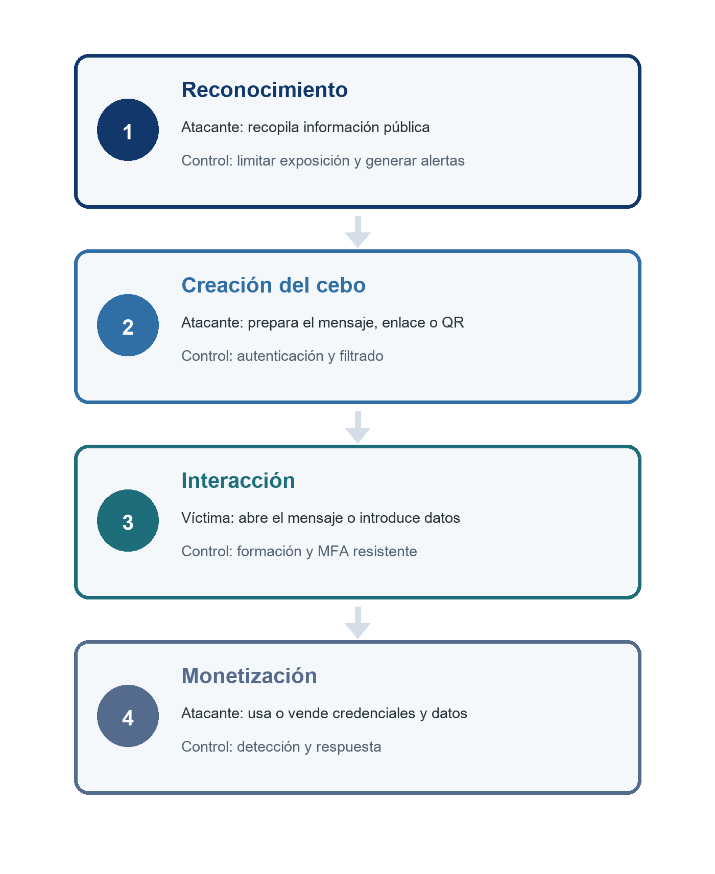
\includegraphics[width=0.86\textwidth]{latex_figures/figura_2_1.png}
  \caption[Fases de un ataque de phishing.]{Fases de un ataque de phishing. Fuente: elaboración propia, adaptada de Alkhalil et al. (2021) y MITRE ATT\&CK (2025). La secuencia relaciona las acciones del atacante y de la víctima con los controles defensivos.}
  \label{fig:2-1}
\end{figure}

\subsection{Preparación y Recopilación de Información (Reconocimiento)}

Esta fase inicial es fundamental para la personalización y efectividad del ataque. El atacante realiza una investigación exhaustiva sobre el objetivo, ya sea un individuo, organización o grupo amplio. Esto incluye la recopilación de datos públicos o filtrados, como correos electrónicos, perfiles en redes sociales, estructuras organizativas o vulnerabilidades técnicas conocidas.

\begin{itemize}
  \item Actividades clave: Análisis de fuentes abiertas (OSINT, por sus siglas en inglés), como LinkedIn para spear phishing o bases de datos de brechas pasadas (p. ej., Have I Been Pwned). En ataques masivos, se usan bots para escanear listas de emails.
  \item Ejemplo: En un spear phishing corporativo, el atacante podría mapear la jerarquía de una empresa para targeting de ejecutivos (whaling).
  \item Duración y riesgos: La fase de reconocimiento puede prolongarse y no siempre deja señales visibles para la organización. El DBIR 2025 identifica el abuso de credenciales como uno de los vectores iniciales más frecuentes, lo que refuerza la necesidad de limitar la exposición pública y vigilar credenciales comprometidas (Verizon, 2025).
\end{itemize}

Interrumpir esta fase mediante políticas de privacidad y monitoreo de datos expuestos es un primer nivel de defensa.

\subsection{Creación y Lanzamiento del Cebo (Setup y Ataque)}

Una vez identificados los vectores de amenaza, el atacante diseña el "cebo" ---el mensaje o vector de entrega--- para que parezca legítimo y urgente. Aquí se aprovecha la ingeniería social para evadir filtros de spam y generar confianza.

\begin{itemize}
  \item Actividades clave: Creación de emails falsos, sitios web clonados (usando kits de phishing como Evilginx) o mensajes en otros canales (SMS para smishing, llamadas para vishing). Se incorporan elementos como logos robados, URLs acortadas o adjuntos maliciosos.
  \item Ejemplo: Un email simulando un banco que advierte de "actividad sospechosa" con un enlace a un sitio falso, o un QR code en un cartel físico que redirige a malware (quishing).
  \item Técnicas avanzadas: Uso de homógrafos (p. ej., un dominio visualmente parecido a paypal.com que sustituye la segunda letra a latina por una a cirílica, U+0430) o envenenamiento de DNS para redirigir tráfico (Imperva, 2023).
\end{itemize}

Esta fase es crítica porque la credibilidad del mensaje y su similitud con comunicaciones reales condicionan la interacción de la víctima. En el DBIR 2025, el phishing figura como vector inicial en el 16 \% de las brechas del subconjunto analizado para este indicador, que excluye errores y uso indebido (9.891 casos). Queda por detrás del abuso de credenciales y de la explotación de vulnerabilidades (Verizon, 2025, p. 10, figura 5).

\begin{figure}[H]
  \centering
  % Datos de Verizon DBIR 2025, p. 10, figura 5. No se infiere una categoría «otros».
\begin{tikzpicture}[x=0.34cm,y=1.05cm,font=\small]
\node[anchor=west,font=\bfseries,color=uemcgreen] at (-12,3.15) {Vectores iniciales seleccionados};
\foreach \x in {0,5,10,15,20,25} {
  \draw[black!12] (\x,-0.55)--(\x,2.55);
  \node[below,font=\footnotesize] at (\x,-0.55) {\x};
}
\fill[uemcgreen] (0,1.74) rectangle (22,2.26);
\fill[tfgblue] (0,0.74) rectangle (20,1.26);
\fill[uemcgreen!70] (0,-0.26) rectangle (16,0.26);
\node[anchor=east,align=right,text width=4cm] at (-0.6,2) {Abuso de credenciales};
\node[anchor=east,align=right,text width=4cm] at (-0.6,1) {Explotación de vulnerabilidades};
\node[anchor=east,align=right,text width=4cm] at (-0.6,0) {Phishing};
\node[anchor=west] at (22.3,2) {22 \%};
\node[anchor=west] at (20.3,1) {20 \%};
\node[anchor=west] at (16.3,0) {16 \%};
\node[font=\footnotesize] at (12.5,-1.13) {Porcentaje del subconjunto de brechas (n=9.891)};
\end{tikzpicture}

  \caption[Vectores iniciales seleccionados del DBIR 2025 (n=9.891).]{Vectores iniciales seleccionados en brechas sin error ni uso indebido. Fuente: elaboración propia con datos de Verizon (2025), p. 10, figura 5.}
  \label{fig:2-2}
\end{figure}

\subsection{Interacción y Explotación (Colección Inicial)}

El objetivo es inducir una acción del usuario, como hacer clic en un enlace, abrir un adjunto o ingresar datos. Aquí ocurre la "mordida" del anzuelo, donde la víctima interactúa con el payload malicioso.

\begin{itemize}
  \item Actividades clave: El usuario puede ser redirigido a un sitio falso para capturar credenciales o inducido a abrir un adjunto malicioso. En ataques de varias etapas, un proxy adversary-in-the-middle (AiTM) puede interceptar tokens de sesión en tiempo real (Kroll, 2025).
  \item Ejemplo: En un ataque de clonación (clone phishing), se duplica un email legítimo previo y se reemplaza un adjunto seguro por uno infectado (Fortinet, 2025).
  \item Factores humanos: La urgencia, el miedo a perder acceso y la apariencia de legitimidad explotan sesgos cognitivos y pueden precipitar una decisión. La formación y la autenticación resistente al phishing reducen el riesgo, pero no eliminan la necesidad de controles técnicos.
\end{itemize}

Esta fase muestra la intersección entre tecnología y psicología: los controles técnicos deben complementarse con formación, autenticación resistente al phishing y mecanismos de detección. El DBIR 2025 sitúa la participación humana en el 60 \% de las brechas analizadas (Verizon, 2025).

\subsection{Adquisición y Monetización de los Datos}

Con los datos en mano, el atacante los procesa y convierte en ganancia. Esta fase cierra el ciclo, pero puede extenderse a ataques secundarios.

\begin{itemize}
  \item Actividades clave: Extracción de credenciales para accesos no autorizados, venta en dark web o uso directo (p. ej., transferencias fraudulentas). En BEC (Business Email Compromise), se roban fondos directamente.
  \item Ejemplo: En la campaña CorruptQR observada por Kroll, documentos de Office con cabeceras dañadas mostraban un código QR tras su reparación; al escanearlo, la víctima era dirigida a una página de phishing orientada al robo de credenciales corporativas y tokens de sesión (Kroll, 2025).
  \item Impacto: El coste económico depende del tipo de incidente y no debe atribuirse íntegramente al phishing. Como referencia general, IBM estimó en 4,44 millones de dólares el coste medio mundial de una brecha de datos en 2025, un 9 \% menos que el año anterior (IBM, 2025).
\end{itemize}

\begingroup
  \arrayrulecolor{uemcgreen}
\begin{table}[H]
  \centering
  \small
  \caption{Indicadores de contexto del phishing y las brechas (2025).}
  \label{tab:2-1}
  \begin{tabularx}{\textwidth}{|X|X|X|X|}
    \hline
    \rowcolor{uemcgreen}
    \textcolor{white}{\textbf{Indicador}} & \textcolor{white}{\textbf{Medida}} & \textcolor{white}{\textbf{Valor}} & \textcolor{white}{\textbf{Fuente}} \\
    \hline
    Actividad observada & Ataques de phishing en Q2 2025 & 1.130.393 & APWG \\
    \hline
    \rowcolor{tablelight}
    Acceso inicial & Phishing en brechas sin error ni uso indebido (n=9.891) & 16 \% & Verizon DBIR \\
    \hline
    Factor humano & Brechas con participación humana & 60 \% & Verizon DBIR \\
    \hline
    \rowcolor{tablelight}
    Impacto general & Coste medio global por brecha & 4,44 M USD & IBM \\
    \hline
  \end{tabularx}
\end{table}
\endgroup

\subsection{Comparación crítica de modelos de fases}

\begingroup
  \arrayrulecolor{uemcgreen}
\begin{table}[H]
  \centering
  \small
  \caption{Comparativa de modelos}
  \label{tab:2-2}
  \begin{tabularx}{\textwidth}{|X|X|X|X|}
    \hline
    \rowcolor{uemcgreen}
    \textcolor{white}{\textbf{Autor/Año}} & \textcolor{white}{\textbf{Nº de fases}} & \textcolor{white}{\textbf{Nombres de las fases}} & \textcolor{white}{\textbf{Ventajas del modelo}} \\
    \hline
    Sulander (2022), Hoxhunt & 3 & Reconocimiento \(\rightarrow\) Elaboración del correo \(\rightarrow\) Ataque/entrega & Centrado en el mensaje \\
    \hline
    \rowcolor{tablelight}
    Alkhalil et al. (2021) & 4 & Planificación \(\rightarrow\) Preparación \(\rightarrow\) Ataque \(\rightarrow\) Adquisición & Explica el proceso completo \\
    \hline
    Adaptación propia & 4 + MITRE & Reconocimiento \(\rightarrow\) Distribución \(\rightarrow\) Interacción \(\rightarrow\) Monetización + tácticas MITRE & Vincula fases y controles \\
    \hline
  \end{tabularx}
\end{table}
\endgroup

\subsection{Puntos de intervención y controles}

\begingroup
  \arrayrulecolor{uemcgreen}
\begin{table}[H]
  \centering
  \small
  \caption{Controles por fase}
  \label{tab:2-3}
  \begin{tabularx}{\textwidth}{|X|X|X|X|}
    \hline
    \rowcolor{uemcgreen}
    \textcolor{white}{\textbf{Fase}} & \textcolor{white}{\textbf{Control preventivo}} & \textcolor{white}{\textbf{Control detectivo}} & \textcolor{white}{\textbf{Herramientas}} \\
    \hline
    Reconocimiento & Monitoreo OSINT & Alertas leaks & Have I Been Pwned \\
    \hline
    \rowcolor{tablelight}
    Distribución & Filtros email (SPF/DKIM/DMARC) & Análisis QR & Mimecast \\
    \hline
    Interacción & MFA resistente AiTM & Monitoreo clics & Microsoft Defender \\
    \hline
    \rowcolor{tablelight}
    Monetización & Detección anomalías & Análisis exfiltración & SIEM (Splunk, QRadar) \\
    \hline
  \end{tabularx}
\end{table}
\endgroup

Este modelo de cuatro fases no es rígido; en ataques sofisticados, se solapan o iteran. Entenderlas es esencial para prototipos de detección, como los basados en ML que analizan patrones en la fase 2 (Alkhalil et al., 2021). Estas fases ilustran cómo el phishing ha evolucionado de ataques rudimentarios a campañas orquestadas, sentando las bases para discutir sus tipos y evolución histórica en las siguientes secciones.

\section{Tipos, clasificación y evolución de los ataques de phishing}

\subsection{Introducción a la clasificación}

Aunque el objetivo final del phishing es siempre el mismo ---obtener información sensible o acceso no autorizado explotando la confianza humana---, la forma de llevarlo a cabo ha diversificado enormemente en los últimos años. En la actualidad, los ataques se clasifican principalmente según tres ejes: el canal o vector empleado, el grado de personalización del ataque y la técnica de explotación utilizada. Esta triple clasificación permite comprender mejor la evolución del fenómeno y anticipar las tendencias futuras.

\subsection{Clasificación según el vector de entrega}

El correo electrónico continúa siendo un canal central del phishing, aunque las campañas combinan cada vez más mensajes, páginas falsas, códigos QR y fraude de correo corporativo. En el segundo trimestre de 2025, APWG declaró 1.130.393 ataques de phishing\footnote{Se reproduce el total trimestral declarado por APWG. La tabla mensual de la p. 3 suma 1.050.031; el informe no explica esta discrepancia y no se dispone de los datos originales para reconciliarla.} y documentó el uso de códigos QR contra 1.642 marcas (Anti-Phishing Working Group, 2025).

Los mensajes SMS (smishing), las llamadas telefónicas (vishing), las redes sociales y los códigos QR amplían los canales de entrega. Kroll observó en 2024 campañas que empleaban mensajes en redes sociales y documentos reparables que revelaban códigos QR, mientras que APWG dedicó en 2025 un seguimiento específico a los ataques mediante QR (Kroll, 2025; Anti-Phishing Working Group, 2025).

Otros vectores menos frecuentes pero en ascenso son el phishing a través de redes sociales (mensajes privados en LinkedIn, WhatsApp Business o Telegram), el envenenamiento de resultados de búsqueda (SEO poisoning) y el pharming o manipulación de resolución DNS.

\subsection{Clasificación según el grado de personalización y objetivo}

En función del nivel de targeting distinguimos varios tipos claramente diferenciados:

\begin{itemize}
  \item Phishing masivo o genérico: campañas de gran volumen que reutilizan mensajes similares. Su coste reducido permite mantenerlas incluso cuando solo una fracción pequeña de los destinatarios interactúa.
  \item Spear-phishing: ataque dirigido contra una persona o un grupo reducido. Requiere investigación previa (OSINT) y mensajes adaptados al contexto, por lo que suele resultar más persuasivo que una campaña genérica.
  \item Whaling o CEO-fraud: variante del spear-phishing dirigida a altos ejecutivos o perfiles financieros. Puede producir pérdidas elevadas cuando deriva en fraude de correo corporativo, aunque el impacto varía ampliamente entre incidentes (Federal Bureau of Investigation, 2024).
  \item Clone phishing: se toma un correo legítimo previamente recibido por la víctima y se modifica un enlace o adjunto. Al conservar elementos de una conversación real, puede aumentar la confianza inicial.
  \item Adversary-in-the-Middle (AiTM): técnica que utiliza proxies inversos para interceptar la autenticación en tiempo real y capturar tokens de sesión incluso cuando la víctima emplea determinados métodos de autenticación multifactor. Constituye un riesgo relevante para servicios corporativos en la nube (Kroll, 2025).
\end{itemize}

\subsection{Clasificación según la técnica de explotación}

El tercer eje clasifica los ataques según la técnica de explotación, con independencia del canal de entrega o del nivel de personalización. Entre las tendencias recientes destacan el uso abusivo de inteligencia artificial generativa, la oferta de kits como servicio y las técnicas orientadas al robo de tokens:

\begin{enumerate}
  \item Inteligencia artificial generativa: los modelos de lenguaje pueden ayudar a redactar mensajes fluidos, adaptar el tono al contexto y producir contenido web. Su resultado depende de la información y de las instrucciones disponibles, y no elimina otros indicios técnicos del ataque.
  \item Phishing-as-a-Service (PhaaS): plataformas que empaquetan plantillas, alojamiento y mecanismos de evasión, reduciendo la barrera de entrada para campañas sofisticadas. Kroll relacionó CorruptQR con la plataforma ONNX y observó otros kits dirigidos a cuentas Microsoft 365 (Kroll, 2025).
  \item Bypass de MFA mediante robo de tokens: los proxies adversary-in-the-middle pueden capturar cookies o tokens de sesión después de una autenticación válida. Por ello se recomiendan métodos resistentes al phishing, como FIDO, junto con controles de acceso condicional (Kroll, 2025).
\end{enumerate}

\subsection{Evolución histórica resumida}

El phishing ha pasado por varias etapas claramente diferenciadas:

\begin{itemize}
  \item 1995-2003: orígenes en AOL y primeros ataques masivos a PayPal.
  \item 2004-2010: aparición de kits (Rock Phish, Avalanche) y profesionalización.
  \item 2011-2016: auge del spear-phishing y del ransomware entregado vía phishing.
  \item 2016-2020: explosión del Business Email Compromise (BEC).
  \item 2020-2022: pandemia y boom de smishing/vishing.
  \item 2022-2025: expansión de la IA generativa, AiTM, quishing y PhaaS, con una mayor combinación de canales, automatización y servicios criminales.
\end{itemize}

En tres décadas, el phishing ha pasado de campañas rudimentarias a operaciones criminales organizadas que combinan automatización, ingeniería social y servicios comercializados en mercados clandestinos.

\subsection{Impacto actual (2025)}

El volumen sigue siendo elevado: APWG declaró 1.130.393 ataques de phishing en el segundo trimestre de 2025. En España, INCIBE gestionó 97.348 incidentes de ciberseguridad durante 2024, incluidos 21.571 casos de phishing. Como indicador económico general, no específico de phishing, IBM situó el coste medio mundial de una brecha en 4,44 millones de dólares en 2025 (Anti-Phishing Working Group, 2025; Instituto Nacional de Ciberseguridad, 2025; IBM, 2025).

Este panorama justifica complementar los filtros de correo y las listas negras con sistemas capaces de analizar el contexto, el comportamiento y la intención del mensaje, objetivo principal del presente trabajo.

\section{La ingeniería social como fundamento psicológico y sociotécnico del phishing}

Aunque el phishing se manifiesta a través de medios técnicos ---correo electrónico, SMS, sitios web falsos o códigos QR---, su eficacia depende en gran medida de la explotación de factores cognitivos, emocionales y sociales. Por ello, la ingeniería social constituye un componente central del fenómeno (Hadnagy, 2018).

\subsection{Principios psicológicos fundamentales explotados}

Los atacantes diseñan sus campañas apoyándose en principios psicológicos bien documentados, muchos de ellos identificados originalmente por Robert Cialdini (1984) y posteriormente validados en el ámbito de la ciberseguridad:

\begingroup
  \arrayrulecolor{uemcgreen}
\begin{table}[H]
  \centering
  \small
  \caption{Aplicación de los principios de Cialdini en campañas de phishing.}
  \label{tab:2-4}
  \begin{tabularx}{\textwidth}{|X|X|X|}
    \hline
    \rowcolor{uemcgreen}
    \textcolor{white}{\textbf{Principio}} & \textcolor{white}{\textbf{Aplicación habitual en phishing}} & \textcolor{white}{\textbf{Riesgo para la víctima}} \\
    \hline
    Autoridad & Suplantación de bancos, administraciones, dirección o proveedores & Reduce el cuestionamiento de la solicitud \\
    \hline
    \rowcolor{tablelight}
    Urgencia / escasez & Plazos breves, bloqueo de cuentas o falsas oportunidades & Favorece decisiones precipitadas \\
    \hline
    Reciprocidad & Regalos, descuentos o supuestas actualizaciones gratuitas & Normaliza la primera interacción \\
    \hline
    \rowcolor{tablelight}
    Compromiso y coherencia & Secuencias que comienzan con una acción pequeña & Aumenta la probabilidad de continuar \\
    \hline
    Prueba social & Avisos sobre acciones atribuidas a otros usuarios & Hace que la petición parezca habitual \\
    \hline
    \rowcolor{tablelight}
    Simpatía & Identidades conocidas, tono cercano o afinidad profesional & Incrementa la confianza inicial \\
    \hline
  \end{tabularx}
\end{table}
\endgroup

\subsection{Sesgos cognitivos específicos explotados}

Más allá de los principios de influencia, los atacantes aprovechan sesgos cognitivos automáticos (Kahneman, 2011; Tversky \& Kahneman, 1974) que operan a nivel Sistema 1 (rápido, intuitivo):

\begin{itemize}
  \item Sesgo de anclaje: el usuario ancla su percepción en el remitente aparentemente legítimo.
  \item Efecto de mera exposición: cuanto más parecido sea el dominio o el diseño al original, mayor confianza genera.
  \item Aversión a la pérdida (loss aversion): el miedo a perder el acceso a una cuenta o sufrir una penalización puede pesar más que una ganancia equivalente y precipitar la respuesta.
  \item Carga de atención: revisar muchos mensajes exige atención sostenida. Como criterio de diseño del prototipo, se muestran señales concretas para ayudar al usuario a revisar cada decisión.
\end{itemize}

La combinación de urgencia, autoridad y prueba social puede elevar la persuasión del mensaje. Este efecto depende del contexto, de la experiencia previa y de las diferencias individuales, por lo que no debe expresarse como una tasa universal de éxito (Heiding et al., 2024).

\subsection{El impacto de la inteligencia artificial generativa en la ingeniería social (2023-2025)}

La disponibilidad de modelos de lenguaje grandes (LLM) ha introducido cambios cualitativos en la preparación de mensajes de ingeniería social:

\begin{itemize}
  \item Reducción de indicadores lingüísticos tradicionales: los modelos generativos pueden producir mensajes fluidos y disminuir errores gramaticales o construcciones extrañas que antes facilitaban la detección (Heiding et al., 2024).
  \item Personalización contextual: los modelos de lenguaje pueden adaptar el tono, incorporar información pública y reproducir terminología propia de un sector, aunque la calidad depende de los datos y de las instrucciones disponibles.
  \item Generación dinámica de narrativas: las herramientas generativas pueden producir y adaptar textos con rapidez. Su uso abusivo reduce el esfuerzo de personalización, aunque no garantiza que el mensaje resulte creíble ni eficaz.
\end{itemize}

Heiding et al. (2024) compararon, con 112 participantes, mensajes genéricos, mensajes generados por GPT-4, mensajes elaborados manualmente con V-Triad y una combinación de ambos. La eficacia varió entre condiciones; el estudio no demuestra una superioridad general de la IA frente a autores humanos. Sus resultados corresponden a ese diseño experimental y no constituyen una tasa universal de éxito.

\subsection{Consecuencias organizativas y humanas}

El Verizon DBIR 2025 sitúa la participación humana en el 60 \% de las brechas analizadas. En España, el 33 \% de los usuarios que contactaron con la línea 017 indicó haber recibido algún intento de phishing, vishing o smishing durante 2024 (Verizon, 2025; Instituto Nacional de Ciberseguridad, 2025).

Este factor humano no es estático: la fatiga por alerta, la sobrecarga de correo y la normalización del trabajo remoto reducen la atención sostenida. Los informes de industria señalan además que determinados perfiles, como finanzas, recursos humanos o dirección, reciben un volumen desproporcionado de ataques dirigidos (Proofpoint, 2025).

\subsection{Implicaciones para la detección}

La dimensión psicológica del phishing implica que una solución eficaz debe combinar el análisis técnico con señales del contexto humano. Los sistemas basados únicamente en características estáticas de URL o contenido pueden degradarse cuando cambian las campañas o se emplea texto generado (Alghenaim et al., 2025; Heiding et al., 2024).

Por tanto, entre las líneas de evolución de la detección se encuentran los modelos que incorporan:

\begin{itemize}[nosep]
  \item Análisis semántico profundo del texto (transformers, LLMs).
  \item Modelado del comportamiento del usuario (UEBA).
  \item Detección de intención y manipulación psicológica mediante NLP avanzado.
\end{itemize}

Estas líneas fundamentan el estado del arte y el prototipo de las siguientes secciones.

\chapter{Estado del arte en técnicas de detección y prevención de phishing basadas en Machine Learning y Deep Learning (2018-2025)}

La detección de phishing ha evolucionado desde reglas y listas de bloqueo hacia modelos de machine learning y deep learning capaces de combinar rasgos de URL, contenido, cabeceras y contexto. Las cifras publicadas no son directamente comparables porque varían el corpus, el equilibrio de clases, la partición de datos y la definición de phishing; por ello, esta revisión prioriza las aportaciones y limitaciones de cada enfoque sobre una clasificación basada únicamente en accuracy (Thakur et al., 2023; Alghenaim et al., 2025).

La sección revisa trabajos académicos e informes técnicos entre 2018 y 2025. Se organiza en enfoques clásicos, deep learning, transformers, métodos híbridos y limitaciones, y utiliza las revisiones citadas para contextualizar estudios representativos sin presentar sus métricas como si procedieran de un único benchmark.

\section{Evolución de los enfoques de detección}

La revisión se organiza en tres periodos orientativos. Las líneas se solapan: esta agrupación no implica que un enfoque sustituya por completo a los anteriores:

\begin{enumerate}
  \item 2019-2021: Enfoques clásicos basados en características manuales. Random Forest, SVM y otros clasificadores trabajan con URL, HTML, cabeceras y variables léxicas. Son rápidos y relativamente explicables, pero dependen de rasgos que pueden envejecer cuando cambian las tácticas.
  \item 2022-2023: Consolidación del deep learning. CNN, LSTM y modelos preentrenados reducen parte de la ingeniería manual y aprenden patrones en URLs o texto. Su comparación sigue limitada por corpus distintos y por evaluaciones realizadas en entornos controlados.
  \item 2024-2025: Transformers y modelos de lenguaje. Los trabajos recientes estudian clasificación zero-shot, ajuste fino, prompt engineering y explicaciones generadas por LLM. El potencial es alto, pero la precisión, la fidelidad de las explicaciones, el coste y la privacidad no mejoran siempre de forma simultánea (Koide et al., 2024; Trad \& Chehab, 2024; Kuikel et al., 2025).
\end{enumerate}

Esta evolución refleja el paso de reglas fijas a modelos que aprenden representaciones más ricas. No elimina la utilidad de los enfoques clásicos: en despliegues locales, la velocidad, la trazabilidad y el coste siguen siendo criterios relevantes.

\section{Enfoques clásicos y primeras redes profundas (2018-2022)}

Este bloque reúne clasificadores con rasgos diseñados manualmente y primeras aproximaciones de aprendizaje profundo. La distinción permite situar las CNN y las redes adversariales en su categoría, aunque compartan periodo de publicación con métodos clásicos.

\begingroup
  \arrayrulecolor{uemcgreen}
\begin{table}[H]
  \centering
  \small
  \caption{Comparativa de enfoques clásicos y primeras redes profundas.}
  \label{tab:3-1}
  \begin{tabularx}{\textwidth}{|X|X|X|X|X|X|}
    \hline
    \rowcolor{uemcgreen}
    \textcolor{white}{\textbf{Año}} & \textcolor{white}{\textbf{Trabajo}} & \textcolor{white}{\textbf{Enfoque}} & \textcolor{white}{\textbf{Objeto}} & \textcolor{white}{\textbf{Aportación}} & \textcolor{white}{\textbf{Limitación}} \\
    \hline
    2018 & Hutchinson et al. & Random Forest & Sitios web & Muestra la utilidad de rasgos de URL y página & Depende de variables diseñadas manualmente \\
    \hline
    \rowcolor{tablelight}
    2020 & Yerima y Alzaylaee & Red convolucional & URLs y páginas & Aprende representaciones con menos ingeniería manual & No cubre por sí sola la semántica completa del correo \\
    \hline
    2020 & AlEroud y Karabatis & Red adversarial & Evasión de detectores & Estudia robustez frente a ejemplos generados & La generalización fuera del laboratorio es difícil \\
    \hline
    \rowcolor{tablelight}
    2022 & Sánchez-Paniagua et al. & Dataset multipropósito & Sitios web & Facilita comparaciones reproducibles & No representa todos los canales de phishing \\
    \hline
  \end{tabularx}
\end{table}
\endgroup

\begin{center}
  \footnotesize (Fuentes: Hutchinson et al., 2018; Yerima \& Alzaylaee, 2020; AlEroud \& Karabatis, 2020; Sánchez-Paniagua et al., 2022).
\end{center}

Los enfoques clásicos extraen características de URLs, páginas, cabeceras o texto y las proporcionan a clasificadores supervisados. Los modelos que aprenden representaciones directamente de la URL reducen parte de esa ingeniería manual (Le et al., 2018), pero su rendimiento también puede caer cuando cambia la distribución o el atacante modifica los rasgos esperados.

Yerima y Alzaylaee (2020) aplicaron redes convolucionales a la detección de phishing, mientras que AlEroud y Karabatis (2020) estudiaron ataques adversariales contra detectores. En conjunto, estos trabajos desplazan el foco desde la precisión estática hacia la capacidad de aprender representaciones y resistir evasiones.

Sánchez-Paniagua et al. (2022) publicaron un dataset multipropósito y características de tecnologías web para facilitar comparaciones reproducibles. La limitación común de esta generación es que un buen resultado sobre páginas o URLs no demuestra por sí solo el comportamiento ante correos nuevos, idiomas distintos o campañas generadas por IA.

\section{Técnicas de Deep Learning y Transformers (2023-2025)}

Los avances recientes enfatizan multimodalidad y zero-shot, con énfasis en LLMs para detección semántica.

\begingroup
  \arrayrulecolor{uemcgreen}
\begin{table}[htbp]
  \centering
  \small
  \caption{Comparativa de técnicas de deep learning y transformers.}
  \label{tab:3-2}
  \begin{tabularx}{\textwidth}{|X|X|X|X|X|X|}
    \hline
    \rowcolor{uemcgreen}
    \textcolor{white}{\textbf{Año}} & \textcolor{white}{\textbf{Trabajo}} & \textcolor{white}{\textbf{Enfoque}} & \textcolor{white}{\textbf{Objeto}} & \textcolor{white}{\textbf{Aportación}} & \textcolor{white}{\textbf{Limitación}} \\
    \hline
    2023 & Thakur et al. & Revisión sistemática & Correo & Sintetiza arquitecturas de deep learning & Los datasets y métricas son heterogéneos \\
    \hline
    \rowcolor{tablelight}
    2023 & Wang et al. & Modelo preentrenado & URLs & Explora transferencia y detección a gran escala & Se centra en la URL, no en el mensaje completo \\
    \hline
    2024 & Altwaijry et al. & Comparativa DL & Correo & Compara varias arquitecturas sobre una misma tarea & El resultado depende del corpus evaluado \\
    \hline
    \rowcolor{tablelight}
    2024 & Koide et al. & LLM zero-shot & Correo & Evalúa detección sin ajuste específico & Coste, privacidad y reproducibilidad \\
    \hline
    2024 & Rojas-Galeano & LLM zero-shot & Spam & Analiza transferencia entre modelos preentrenados & Spam y phishing no son categorías equivalentes \\
    \hline
    \rowcolor{tablelight}
    2024 & Uddin et al. & Transformer explicable & Correo & Relaciona predicción con términos relevantes & Preprint pendiente de validación más amplia \\
    \hline
    2025 & Kuikel et al. & LLM + explicaciones & Correo & Compara precisión y alineación de explicaciones & Existe un compromiso entre acierto y fidelidad \\
    \hline
    \rowcolor{tablelight}
    2025 & Alghenaim et al. & Revisión del estado del arte & Detección con IA & Resume tendencias, riesgos y líneas abiertas & No es un clasificador evaluado de forma original \\
    \hline
  \end{tabularx}
\end{table}
\endgroup

\begin{center}
  \footnotesize (Fuentes: Thakur et al., 2023; Wang et al., 2023; Altwaijry et al., 2024; Koide et al., 2024; Rojas-Galeano, 2024; Uddin et al., 2024; Kuikel et al., 2025; Alghenaim et al., 2025).
\end{center}

Los trabajos recientes amplían el objeto de análisis, pero difieren en corpus, tarea y protocolo de evaluación. La tabla resume su aportación principal sin mezclar resultados que no proceden del mismo benchmark.

Las revisiones de Thakur et al. (2023) y Alghenaim et al. (2025) describen una transición hacia redes profundas, modelos preentrenados y combinaciones de texto, URL y metadatos. Este avance reduce parte de la ingeniería manual, aunque mantiene problemas de comparabilidad y deriva temporal.

Altwaijry et al. (2024) compararon modelos de deep learning para correo y Koide et al. (2024) exploraron un detector basado en modelos de lenguaje. Ambos trabajos muestran el interés por incorporar contexto semántico, pero no justifican trasladar una cifra de accuracy a otros corpus o entornos.

Rojas-Galeano (2024) estudió clasificación zero-shot de spam, una tarea próxima pero no idéntica al phishing. Uddin et al. (2024) abordaron la explicabilidad con transformers y Kuikel et al. (2025) observaron que una mejor alineación entre predicción y explicación no implica necesariamente mayor precisión. Esta tensión es central para sistemas de apoyo a la decisión.

\section{Enfoques híbridos y basados en comportamiento (UEBA)}

Los enfoques híbridos combinan señales estructurales, contenido y comportamiento para aportar contexto que una única fuente no contiene. La integración puede mejorar cobertura, pero aumenta la complejidad de datos, despliegue y evaluación.

\begin{itemize}
  \item Híbridos semánticos e ingeniería social: combinan representaciones del texto con señales de urgencia, autoridad o solicitud de credenciales. Su principal reto es demostrar que esas señales generalizan fuera del corpus de entrenamiento.
  \item Multimodal: fusiona texto, URL, imágenes y metadatos. Puede detectar señales complementarias, aunque exige datasets alineados y eleva el coste de entrenamiento e inferencia.
  \item Zero-shot: utiliza modelos preentrenados sin ajuste específico. Es útil para explorar ataques emergentes, pero introduce variabilidad, coste y posibles transferencias de datos a servicios externos.
  \item Prevención proactiva: UEBA analiza cambios de comportamiento y anomalías de acceso. Complementa la inspección del mensaje, aunque requiere telemetría organizativa que queda fuera del alcance de este prototipo.
\end{itemize}

La literatura reciente presenta los métodos híbridos como una línea prometedora, pero subraya la necesidad de evaluar cada componente y evitar que la complejidad oculte qué señal sostiene la decisión (Alghenaim et al., 2025; Popescul y Radu, 2025).

\section{Limitaciones actuales de los enfoques}

Aunque distintos trabajos publican resultados elevados en sus propios corpus, persisten desafíos que impiden compararlos directamente:

\begin{enumerate}
  \item Datasets desfasados: muchos corpus no reflejan campañas recientes, IA generativa, quishing ni deriva de dominios. Un resultado interno elevado puede degradarse ante ataques nuevos.
  \item Coste y latencia: los modelos grandes exigen más memoria, cómputo o llamadas a servicios externos; los modelos locales ligeros ofrecen mayor control y reproducibilidad.
  \item Multilingüismo y sesgo: el predominio de corpus en inglés dificulta trasladar resultados al español y a contextos culturales diferentes.
  \item Robustez adversarial: homógrafos, ofuscación, cambios de plantilla y texto generado pueden eludir patrones aprendidos. Pocos trabajos evalúan de forma comparable estas evasiones.
  \item Explicabilidad: una explicación generada no garantiza fidelidad al proceso de decisión. Debe distinguirse entre texto persuasivo y evidencia verificable del modelo.
\end{enumerate}

La revisión bibliométrica de Popescul y Radu (2025) confirma el crecimiento de ML, deep learning y modelos híbridos, y señala como líneas abiertas la adaptación a nuevos vectores, la robustez y la integración organizativa.

\section{Conclusiones del estado del arte y hueco de investigación}

La literatura reciente sitúa los transformers y los LLM entre las líneas activas de investigación, pero advierte que los resultados de entornos controlados no son directamente comparables. Persisten tres huecos relevantes:

\begin{enumerate}
  \item Falta de fine-tuning open-source para español/multilingüe
  \item Escasa integración de detección psicológica (Cialdini) en LLMs
  \item Evaluación limitada contra ataques GenAI en tiempo real.
\end{enumerate}

\chapter{Metodología y planificación}

Este capítulo describe el enfoque metodológico seguido para el desarrollo del prototipo, así como la planificación temporal del proyecto y las herramientas empleadas. El trabajo se ha desarrollado a lo largo del curso académico 2025-2026, distribuyendo las actividades de análisis y documentación en el primer cuatrimestre y las de implementación y validación en el segundo.

\section{Enfoque metodológico}

El proyecto se ha desarrollado siguiendo una metodología iterativa e incremental, combinada con una revisión bibliográfica continua. Cada iteración añade una capacidad nueva al sistema y se cierra con la ejecución de la suite de pruebas, de modo que el prototipo permanece en un estado funcional durante todo el proceso.

La fase inicial, desarrollada entre octubre y diciembre de 2025, se dedicó al estudio del contexto del problema y a la revisión de la literatura académica (IEEE, arXiv y Springer) y de los informes de industria citados en el estado del arte. Esta etapa permitió identificar las técnicas de detección más relevantes, delimitar el hueco de investigación y definir los objetivos específicos y el alcance del sistema.

Una vez consolidado el marco teórico, se adoptó un enfoque de desarrollo en espiral adaptado al tamaño del trabajo, llevado a cabo entre febrero y junio de 2026. Primero se construyó un núcleo heurístico explicable, después se añadió el clasificador neuronal TF-IDF + MLP y, a continuación, se separaron el backend HTTP central y los clientes Streamlit, extensión y monitor. Gmail aporta mensajes autorizados y Telegram actúa como salida opcional; ambos se coordinan alrededor del contrato del servidor. Cada avance se cerró con la ejecución de la suite de pruebas, manteniendo el prototipo en un estado funcional durante todo el proceso.

Durante el desarrollo se emplearon herramientas de inteligencia artificial generativa como apoyo para consultas técnicas puntuales, diagnóstico y resolución de errores, revisión de fragmentos de código, asistencia en el CSS de la interfaz y revisión de documentación. Antes de incorporar los cambios se realizaron las comprobaciones correspondientes; las decisiones técnicas, la interpretación de los resultados y la responsabilidad final corresponden al autor. Estas herramientas no se utilizaron como fuente académica: los contenidos teóricos se contrastaron y citaron mediante sus fuentes originales.

La gestión del proyecto se apoyó en el control de versiones Git y en la plataforma GitHub como repositorio remoto. El desarrollo se organizó por funcionalidades y cada hito se validó mediante pruebas automatizadas antes de integrarse en la versión de trabajo, con especial atención a las funciones críticas de detección, normalización y persistencia de modelos.

\section{Planificación temporal del proyecto}

La planificación inicial se distribuyó en siete fases repartidas a lo largo del curso académico. La tabla siguiente resume la planificación temporal, las actividades principales de cada fase y el entregable asociado. Las fases de análisis y documentación se concentraron en el primer cuatrimestre, mientras que la implementación del prototipo y su validación se desarrollaron en el segundo.

\begingroup
  \arrayrulecolor{uemcgreen}
\begin{table}[htbp]
  \centering
  \small
  \caption{Planificación inicial del proyecto.}
  \label{tab:4-1}
  \begin{tabularx}{\textwidth}{|X|X|X|X|}
    \hline
    \rowcolor{uemcgreen}
    \textcolor{white}{\textbf{Fase}} & \textcolor{white}{\textbf{Periodo}} & \textcolor{white}{\textbf{Actividades principales}} & \textcolor{white}{\textbf{Entregable}} \\
    \hline
    Fase 1: Análisis del contexto y estado del arte & Octubre - diciembre 2025 & Revisión bibliográfica, análisis del phishing, sus tipologías, la ingeniería social y las técnicas de detección. & Marco teórico y estado del arte \\
    \hline
    \rowcolor{tablelight}
    Fase 2: Diseño funcional y modular & Enero - febrero 2026 & Definición del alcance de la aplicación web, separación de responsabilidades y selección de tecnologías. & Especificación funcional y diseño modular \\
    \hline
    Fase 3: Motor heurístico & Febrero - marzo 2026 & Implementación del analizador, señales de cabeceras, contenido, URLs y HTML, y cálculo del riesgo. & Núcleo heurístico con pruebas \\
    \hline
    \rowcolor{tablelight}
    Fase 4: Clasificador neuronal & Marzo - abril 2026 & Pipeline TF-IDF + MLP, entrenamiento en español e inglés y comparación de configuraciones. & Modelos neuronales entrenables \\
    \hline
    Fase 5: Aplicación web & Abril - mayo 2026 & Desarrollo de las vistas Streamlit de inicio, configuración, detección, monitorización y entrenamiento. & Aplicación web funcional \\
    \hline
    \rowcolor{tablelight}
    Fase 6: Integraciones y validación & Mayo - junio 2026 & Integración OAuth con Gmail, alertas de Telegram, pruebas automatizadas y evaluación funcional. & Prototipo integrado y resultados \\
    \hline
    Fase 7: Documentación final & Junio 2026 & Validación final, redacción de la memoria y revisión de la documentación. & Memoria del TFG \\
    \hline
  \end{tabularx}
\end{table}
\endgroup

La planificación inicial terminaba en junio. La versión de entrega incorpora después el entrenamiento reproducible y las mediciones de agosto de 2026, además de la revisión documental y las correcciones del tribunal de septiembre. Las fechas de los artefactos y los informes identifican estas comprobaciones finales; la tabla no debe interpretarse como fecha de cierre de la versión entregada.

La carga de trabajo del segundo cuatrimestre se concentró en el motor heurístico, el clasificador neuronal y el backend central, que reúnen la lógica del prototipo. Después se adaptaron Streamlit, Gmail, la extensión y el monitor como clientes del mismo contrato HTTP. La extensión llama directamente al servidor; el proceso del puerto 8767 se conserva únicamente como proxy de compatibilidad, sin reglas ni modelos propios.

\section{Correspondencia con la propuesta inicial}
\label{sec:estructura-propuesta}

La propuesta aprobada, titulada \emph{Phishing. Técnicas y métodos de ataque y cómo detectarlos}, contemplaba una estructura modificable. La tabla~\ref{tab:estructura-propuesta} conserva los trece bloques y su orden, según el apartado 3.1 de la propuesta (páginas 5--6), e indica su ubicación o tratamiento final. El cuerpo se organiza en siete capítulos. El análisis de técnicas de ataque se integra en el marco teórico y las técnicas de defensa se distribuyen entre el estado del arte y la evaluación del prototipo, distinguiendo la evidencia publicada por terceros de los resultados de este trabajo.

\begin{table}[H]
\centering\small
\caption{Correspondencia entre la estructura prevista y la memoria final.}
\label{tab:estructura-propuesta}
\begin{tabularx}{\textwidth}{|>{\RaggedRight\arraybackslash}p{5.2cm}|>{\RaggedRight\arraybackslash}X|}
\hline
\rowcolor{uemcgreen}\color{white}\bfseries Bloque de la propuesta & \color{white}\bfseries Ubicación y tratamiento final \\\hline
1. Portada & Portada con el título aprobado y los datos de autoría y convocatoria. \\\hline
2. Resumen & Resumen inicial; se añade su versión en inglés. \\\hline
3. Introducción & Capítulo 1: contexto y objetivos; alcance concretado en el capítulo 5. \\\hline
4. Marco teórico & Capítulo 2: concepto, evolución, modalidades, fases e ingeniería social. \\\hline
5. Estado del arte & Capítulo 3: estudios previos, herramientas y enfoques de detección y prevención. \\\hline
6. Metodología y planificación & Capítulo 4: enfoque, tecnologías, flujo de trabajo y planificación. \\\hline
7. Análisis de técnicas de ataque & Integrado en el capítulo 2: tipos, ejemplos y estrategias de ingeniería social. \\\hline
8. Análisis y evaluación de técnicas de defensa & Capítulo 3: comparación bibliográfica de métodos, eficacia y límites; capítulo 6: evaluación propia. \\\hline
9. Diseño y desarrollo de medidas defensivas & Capítulo 5: arquitectura, componentes, reglas e interfaz; ejemplos de uso en el capítulo 6. \\\hline
10. Pruebas, resultados y discusión & Capítulo 6: ejemplos, resultados y límites. La comparación con soluciones existentes se trata bibliográficamente en el capítulo 3. \\\hline
11. Conclusiones & Capítulo 7: logros, cumplimiento parcial y trabajo futuro. \\\hline
12. Bibliografía y anexos & Referencias y anexos A--E: repositorio, extractos de código, uso, lista de verificación y evidencia. Capturas y tablas en los capítulos 5 y 6. \\\hline
13. Glosario & Sección final situada antes de las referencias para facilitar la consulta. \\\hline
\end{tabularx}
\end{table}

Esta reorganización evita duplicar la explicación de los ataques y permite seguir el recorrido desde la amenaza hasta el prototipo y sus resultados. La comparación experimental se limita a los modos heurístico, neuronal y combinado del sistema desarrollado. Las soluciones ajenas se comparan mediante bibliografía; no se ha realizado un benchmark directo de productos comerciales. La reducción de alcance funcional, distinta del cambio de organización, se detalla en el apartado~\ref{sec:objetivos-propuesta}.


\section{Herramientas y tecnologías}

La tabla siguiente recoge las principales herramientas y tecnologías utilizadas durante el desarrollo, junto con el propósito de cada una en el proyecto.

\begingroup
  \arrayrulecolor{uemcgreen}
\begin{table}[H]
  \centering
  \small
  \caption{Herramientas y tecnologías utilizadas.}
  \label{tab:4-2}
  \begin{tabularx}{\textwidth}{|X|X|}
    \hline
    \rowcolor{uemcgreen}
    \textcolor{white}{\textbf{Herramienta / tecnología}} & \textcolor{white}{\textbf{Propósito en el proyecto}} \\
    \hline
    Python 3 & Lenguaje de programación principal del prototipo. \\
    \hline
    \rowcolor{tablelight}
    Streamlit & Interfaz web con vistas de inicio, configuración, detección, monitorización y entrenamiento. \\
    \hline
    BeautifulSoup4 & Procesamiento del HTML incluido en los correos y extracción de señales estructurales. \\
    \hline
    \rowcolor{tablelight}
    NumPy & Operaciones numéricas utilizadas durante el entrenamiento y la evaluación. \\
    \hline
    scikit-learn & Vectorizador TF-IDF, clasificador MLPClassifier y métricas de evaluación. \\
    \hline
    \rowcolor{tablelight}
    joblib & Persistencia en disco de los modelos neuronales entrenados. \\
    \hline
    langdetect & Selección del modelo en español o inglés según el contenido del correo. \\
    \hline
    \rowcolor{tablelight}
    Gmail API (OAuth) & Importación autorizada de correos desde la bandeja del usuario. \\
    \hline
    Bot API de Telegram & Envío opcional de alertas desde la monitorización de Gmail. \\
    \hline
    \rowcolor{tablelight}
    unittest & Pruebas unitarias y de integración de los componentes del prototipo. \\
    \hline
    Git y GitHub & Control de versiones, trazabilidad y respaldo del desarrollo. \\
    \hline
  \end{tabularx}
\end{table}
\endgroup

\section{Validación y control de calidad}

La validación del sistema se realiza en seis niveles complementarios: 94 pruebas Python de componentes e integración, 2 recorridos reales con Chromium, un benchmark reproducible, una calibración bilingüe de 40 casos, 16 EML locales reservados y un diagnóstico de 1.528 textos externos DIFrauD. Un recorrido levanta cliente web y backend separados; otro prueba Gmail, HTTP y Telegram de extremo a extremo con dobles externos. Los EML son sintéticos y DIFrauD conserva riesgo de solapamiento con fuentes de entrenamiento; ninguna cifra se extrapola a producción.

En segundo lugar, la aplicación permite evaluar el clasificador neuronal con un CSV de prueba independiente, separado del conjunto de entrenamiento. La interfaz calcula exactitud, precisión, recall, F1, accuracy balanceada y la matriz de confusión; no se fija una partición automática 70/30 ni se presentan resultados estadísticos sin indicar el conjunto utilizado. En tercer lugar, se comprobaron los flujos funcionales de la aplicación web: análisis de texto pegado y archivos .eml, selección del modelo por idioma, importación mediante Gmail y navegación entre las vistas de detección y entrenamiento. Los resultados reproducibles se presentan en la sección de pruebas y discusión.

\section{Aspectos éticos y de protección de datos}

El tratamiento de los correos electrónicos analizados por el prototipo se plantea conforme al Reglamento General de Protección de Datos (RGPD, Reglamento (UE) 2016/679). El sistema minimiza la información procesada: solo extrae los metadatos y las señales necesarias para la clasificación (cabeceras, remitente, asunto, enlaces y estructura HTML), sin almacenar de forma persistente el contenido íntegro de los mensajes, las credenciales de acceso ni los datos personales de los remitentes.

El acceso a la API de Gmail se realiza mediante OAuth, delegando en Google la autenticación del usuario y evitando el manejo de contraseñas en la aplicación. El prototipo está diseñado para entornos controlados y académicos, con datos de demostración o con el consentimiento explícito del usuario. Los tokens y credenciales se almacenan localmente y quedan excluidos del repositorio. Antes de publicar la aplicación para varios usuarios sería necesario incorporar autenticación, gestión segura de secretos y una política explícita de conservación de datos.

\chapter{Diseño e implementación de la aplicación web}

Tras el análisis teórico de las técnicas de phishing y de los principales enfoques de detección existentes, se ha desarrollado un prototipo funcional orientado al análisis de correos electrónicos sospechosos. El objetivo del sistema no es sustituir a una solución empresarial completa de seguridad, sino demostrar cómo puede combinarse un enfoque heurístico explicable con un clasificador automático basado en aprendizaje supervisado.

El prototipo se centra en el análisis de mensajes desde varios clientes. El origen puede ser texto, EML, Gmail, la extensión o JSON. El cliente transporta la entrada y el backend central extrae cabeceras, remitente, asunto, cuerpo, HTML, enlaces, anclas y adjuntos para generar el riesgo heurístico, neuronal o combinado. La interfaz recibe un contrato ya calculado y se limita a presentarlo.

\section{Alcance del sistema}

El alcance del prototipo se ha delimitado al análisis estático del correo electrónico y de las URLs contenidas en él. El sistema no navega activamente hacia las páginas enlazadas, no descarga contenido externo ni consulta servicios de reputación en tiempo real. La API, la extensión, Streamlit y los procesos de monitorización se mantienen en el entorno local y no convierten el proyecto en un servicio remoto multiusuario.

No obstante, la arquitectura queda preparada para ampliaciones futuras. Podrían añadirse consultas a listas negras públicas, reputación de dominios, validación de certificados TLS, análisis dinámico de páginas o integración con sistemas corporativos de alerta. El prototipo no se plantea, por tanto, como un producto cerrado, sino como una base funcional y extensible.

\section{Requisitos funcionales y no funcionales}

Los requisitos siguientes convierten el alcance descrito en criterios verificables. Los funcionales definen qué debe hacer el prototipo; los no funcionales fijan las condiciones de seguridad, reproducibilidad, mantenibilidad y rendimiento propias de una demostración académica local.

\begingroup
  \arrayrulecolor{uemcgreen}
\begin{table}[H]
  \centering
  \small
  \caption{Requisitos funcionales y no funcionales del prototipo.}
  \label{tab:5-1}
  \begin{tabularx}{\textwidth}{|X|X|X|X|}
    \hline
    \rowcolor{uemcgreen}
    \textcolor{white}{\textbf{Tipo}} & \textcolor{white}{\textbf{ID}} & \textcolor{white}{\textbf{Requisito}} & \textcolor{white}{\textbf{Verificación}} \\
    \hline
    Funcional & RF-01 & Analizar texto, EML y mensajes autorizados de Gmail. & Pruebas de parser, API, Gmail y recorridos Chromium. \\
    \hline
    \rowcolor{tablelight}
    Funcional & RF-02 & Ofrecer modos heurístico, neuronal y combinado. & Evaluación de los tres modos sobre los mismos 16 EML. \\
    \hline
    Funcional & RF-03 & Mostrar puntuación, veredicto, señales y explicación. & Contrato JSON, interfaz y capturas reproducibles. \\
    \hline
    \rowcolor{tablelight}
    Funcional & RF-04 & Mantener una versión activa ES y otra EN en el backend. & Health, metadatos, activación atómica y pruebas. \\
    \hline
    Funcional & RF-05 & Permitir alertas opcionales por Telegram. & Prueba integral Gmail-HTTP-backend-Telegram con dobles. \\
    \hline
    \rowcolor{tablelight}
    No funcional & RNF-01 & Procesar por defecto en loopback y minimizar datos persistidos. & Rutas runtime separadas, OAuth de solo lectura y revisión de secretos. \\
    \hline
    No funcional & RNF-02 & Poder reconstruir entrenamiento y evaluación. & Dependencias fijadas, semillas, SHA-256 y scripts reproducibles. \\
    \hline
    \rowcolor{tablelight}
    No funcional & RNF-03 & Separar presentación, transporte, aplicación y dominio. & Arquitectura modular y suite automatizada. \\
    \hline
    No funcional & RNF-04 & Arrancar y responder con latencia apta para la demo. & Benchmark medido y prueba local de concurrencia. \\
    \hline
  \end{tabularx}
\end{table}
\endgroup

El cumplimiento se evalúa dentro del alcance declarado: no implica eficacia universal, operación multiusuario ni garantías de producción.

\section{Cambios respecto a la propuesta inicial}

La propuesta de octubre de 2025 contemplaba un prototipo con reglas, servicios externos de reputación, comprobación de certificados y la posible utilización de TensorFlow. Durante el desarrollo se ajustó el alcance para priorizar privacidad, seguridad de la evaluación, reproducibilidad local y una arquitectura cliente-servidor con un único modelo compartido.

\begingroup
  \arrayrulecolor{uemcgreen}
\begin{table}[H]
  \centering
  \small
  \caption{Cambios respecto a la propuesta inicial.}
  \label{tab:5-2}
  \begin{tabularx}{\textwidth}{|X|X|X|X|}
    \hline
    \rowcolor{uemcgreen}
    \textcolor{white}{\textbf{Elemento}} & \textcolor{white}{\textbf{Propuesta}} & \textcolor{white}{\textbf{Implementación final}} & \textcolor{white}{\textbf{Justificación}} \\
    \hline
    Aprendizaje & scikit-learn y TensorFlow & TF-IDF + MLPClassifier de scikit-learn & Pipeline ligero, reproducible y suficiente para el alcance; TensorFlow no era necesario. \\
    \hline
    \rowcolor{tablelight}
    Reputación & Listas negras y servicios externos & Listas y señales locales; sin consultas online & Evita enviar URLs sensibles, depender de cuotas o visitar infraestructura potencialmente maliciosa. \\
    \hline
    Certificados & Comprobación de certificados digitales & Sin conexión al destino ni validación TLS & Un EML no acredita el certificado actual del enlace; la comprobación activa queda como trabajo futuro aislado. \\
    \hline
    \rowcolor{tablelight}
    Arquitectura & Interfaz sencilla del prototipo & Clientes HTTP y backend central obligatorio & Una actualización del modelo se aplica a web, extensión y monitor sin distribuir copias. \\
    \hline
  \end{tabularx}
\end{table}
\endgroup

Estos cambios no alteran el objetivo académico de estudiar, implementar y evaluar la detección de phishing. Delimitan qué se demuestra en el prototipo y qué capacidades necesitan infraestructura y controles adicionales.

\subsection{Cumplimiento de los objetivos y desviaciones de alcance}
\label{sec:objetivos-propuesta}

El cumplimiento se valora frente a la propuesta aprobada y no solo frente a los requisitos finales. Sus cinco objetivos académicos (apartado 1, página 4) se corresponden con los contenidos siguientes, manteniendo su orden original:

\begin{enumerate}[leftmargin=*,itemsep=3pt]
\item \textbf{Comprender el funcionamiento, la estructura, las fases y las variantes del phishing.} Se desarrolla en el capítulo 2 mediante conceptos, modalidades y modelos de fases.
\item \textbf{Analizar la evolución de las estrategias de ingeniería social.} El capítulo 2 relaciona la evolución de los ataques con la manipulación, los principios psicológicos y los usos de IA descritos en las fuentes.
\item \textbf{Estudiar métodos de detección mediante software y políticas organizativas, con sus ventajas y límites.} Los controles por fase del capítulo 2 y el estado del arte del capítulo 3 cubren ambos planos; la evaluación propia del capítulo 6 se limita al software desarrollado.
\item \textbf{Desarrollar capacidad crítica para evaluar medidas preventivas en contextos personales, empresariales e institucionales.} Se aborda mediante la comparación bibliográfica y la discusión de límites; no se ha medido la eficacia de esas medidas en organizaciones ni en estudios de campo con usuarios.
\item \textbf{Fomentar el aprendizaje autónomo y aplicar conocimientos teóricos a un problema real de ciberseguridad.} Se materializa en el desarrollo y la evaluación del prototipo (capítulos 4--6), dentro de un entorno académico controlado.
\end{enumerate}

La tabla~\ref{tab:objetivos-propuesta} recoge los cuatro objetivos funcionales del apartado 2 de la propuesta (página 4), en su orden original, y distingue los dos compromisos adicionales de su resumen (página 3). Las recomendaciones preventivas forman parte del alcance inicial, aunque no figuren como una quinta viñeta de objetivos funcionales.

\begin{table}[H]
\centering\small
\caption{Trazabilidad de los objetivos funcionales y compromisos del resumen de la propuesta.}
\label{tab:objetivos-propuesta}
\begin{tabularx}{\textwidth}{|>{\RaggedRight\arraybackslash}p{5.1cm}|>{\RaggedRight\arraybackslash}p{2.5cm}|>{\RaggedRight\arraybackslash}X|}
\hline
\rowcolor{uemcgreen}\color{white}\bfseries Objetivo original & \color{white}\bfseries Estado & \color{white}\bfseries Evidencia y alcance \\\hline
1. Diseñar un prototipo capaz de identificar indicios de phishing en correos electrónicos o URLs mediante análisis de contenido, enlaces y cabeceras. & Parcial & Texto, EML y Gmail; inspección estática de los enlaces del mensaje. No se visita ni se verifica el sitio de destino. \\\hline
2. Implementar un conjunto de reglas y verificaciones heurísticas que permitan evaluar la legitimidad de un mensaje o sitio web. & Parcial & 31 señales del correo y pruebas sobre EML. Proporciona indicios; no acredita la legitimidad de un sitio web. \\\hline
3. Integrar fuentes externas, como listas negras y servicios de comprobación de reputación, para reforzar la fiabilidad del sistema. & No desarrollado & Se emplean listas locales y reglas. No hay consultas a proveedores de reputación ni actualización automática desde fuentes externas. \\\hline
4. Elaborar una interfaz sencilla que facilite la comprensión de los resultados del análisis por parte del usuario. & Implementado & Streamlit y extensión presentan riesgo y explicaciones. Hay pruebas funcionales, sin estudio de usabilidad con participantes. \\\hline
Resumen: comprobaciones de certificados digitales. & No desarrollado & El sistema no conecta con los destinos ni valida sus certificados TLS. \\\hline
Resumen: medidas técnicas y organizativas y guía de buenas prácticas para usuarios y administradores. & Parcial & Controles y recomendaciones en el capítulo 2 y la discusión. No se elaboró una guía independiente para ambos perfiles. \\\hline
\end{tabularx}
\end{table}

La consulta de reputación y la comprobación activa de certificados se excluyeron para mantener un análisis estático reproducible y evitar enviar URLs potencialmente sensibles a terceros o contactar con infraestructura sospechosa. También se evitó incorporar dependencias de cuotas, credenciales y disponibilidad de esos servicios. Estas razones explican la decisión, pero no permiten considerar cumplidos los objetivos excluidos.

La consecuencia es una menor cobertura: no se conoce la reputación actual del destino, su contenido servido en ese momento ni el estado de su certificado. Las listas locales pueden quedar desactualizadas. El sistema aporta indicios del correo recibido; no certifica que una URL sea segura. Incorporar esas capacidades requeriría un módulo de consultas separado, límites de tiempo, controles de privacidad y una evaluación específica. Su mención como trabajo futuro no sustituye esta declaración de incumplimiento parcial.

Gmail, Telegram y la centralización de los modelos amplían las formas de uso del prototipo, pero no compensan por sí mismas la ausencia de reputación online o análisis activo de sitios web. Las medidas preventivas se integraron en la exposición teórica y la discusión, concentrando el desarrollo y la validación en el detector. Por ello, la guía de buenas prácticas anunciada en el resumen quedó sin elaborar como entregable independiente: las recomendaciones están dispersas y no constituyen una guía adaptada y validada para usuarios y administradores. La guía de instalación y uso del anexo C explica el prototipo y no sustituye ese compromiso preventivo.

\subsection{Elección de scikit-learn frente al uso previsto de TensorFlow}
\label{sec:decision-tensorflow}

La propuesta incluía scikit-learn y TensorFlow entre las tecnologías previstas. La implementación final concentra el aprendizaje en un pipeline de scikit-learn con TF-IDF y \texttt{MLPClassifier}. Por tanto, se conserva un clasificador neuronal multicapa, aunque no se utiliza TensorFlow. La selección responde al alcance del experimento: clasificación supervisada de texto mediante una representación léxica fija, dos idiomas y ejecución local sobre CPU.

Esta solución permite reunir vectorización, ajuste y predicción en un mismo pipeline, conservar su configuración y serializarlo con las herramientas ya empleadas por el proyecto. Reduce el número de bibliotecas que deben integrarse y mantiene un procedimiento de entrenamiento común para ambos idiomas. La arquitectura cliente-servidor no depende de esta elección: los clientes reciben el mismo contrato JSON y la implementación del modelo queda encapsulada en el backend.

La contrapartida es la expresividad de la representación elegida. TF-IDF utiliza un vocabulario limitado y n-gramas de una o dos palabras; no incorpora una representación contextual de todo el mensaje ni modela por sí mismo su estructura MIME. El MLP aprende a partir de esos rasgos y depende de la representatividad de los corpus. Las cabeceras y los enlaces estructurados se examinan mediante las reglas, no mediante el vectorizador. Diseñar otra representación o una arquitectura neuronal distinta exigiría nuevas decisiones de datos, entrenamiento y validación.

No se implementó ni se midió un modelo equivalente en TensorFlow. En consecuencia, no se afirma que scikit-learn sea más preciso, rápido o eficiente que TensorFlow. La decisión simplifica la implementación de este prototipo; no establece una superioridad general entre bibliotecas. La exclusión de TensorFlow reduce la exploración de arquitecturas alternativas prevista inicialmente, pero permite mantener el objetivo de estudiar un detector neuronal y compararlo con reglas explicables. Las conclusiones experimentales se refieren exclusivamente a TF-IDF más MLP y a su combinación con la heurística.


\section{Arquitectura general}

La solución adopta una arquitectura cliente-servidor. El navegador se comunica con Streamlit, que actúa como capa de presentación y cliente HTTP del backend central; la extensión y el monitor consumen esa misma API. Solo backend\_server.py normaliza, analiza, entrena y mantiene los modelos activos. Cada instalación conserva credenciales y preferencias en runtime/client, mientras el backend es propietario de los ajustes y modelos de runtime/server; la interfaz administra los valores centrales por API, no mediante acceso directo al disco. En la configuración académica ambos lados se ejecutan en el mismo equipo y sobre loopback, pero son procesos y responsabilidades independientes. Para una demostración en la red local puede exponerse temporalmente solo Streamlit en 0.0.0.0:8501; el backend permanece en 127.0.0.1:8766 y no se publica.

\begin{figure}[H]
  \centering
  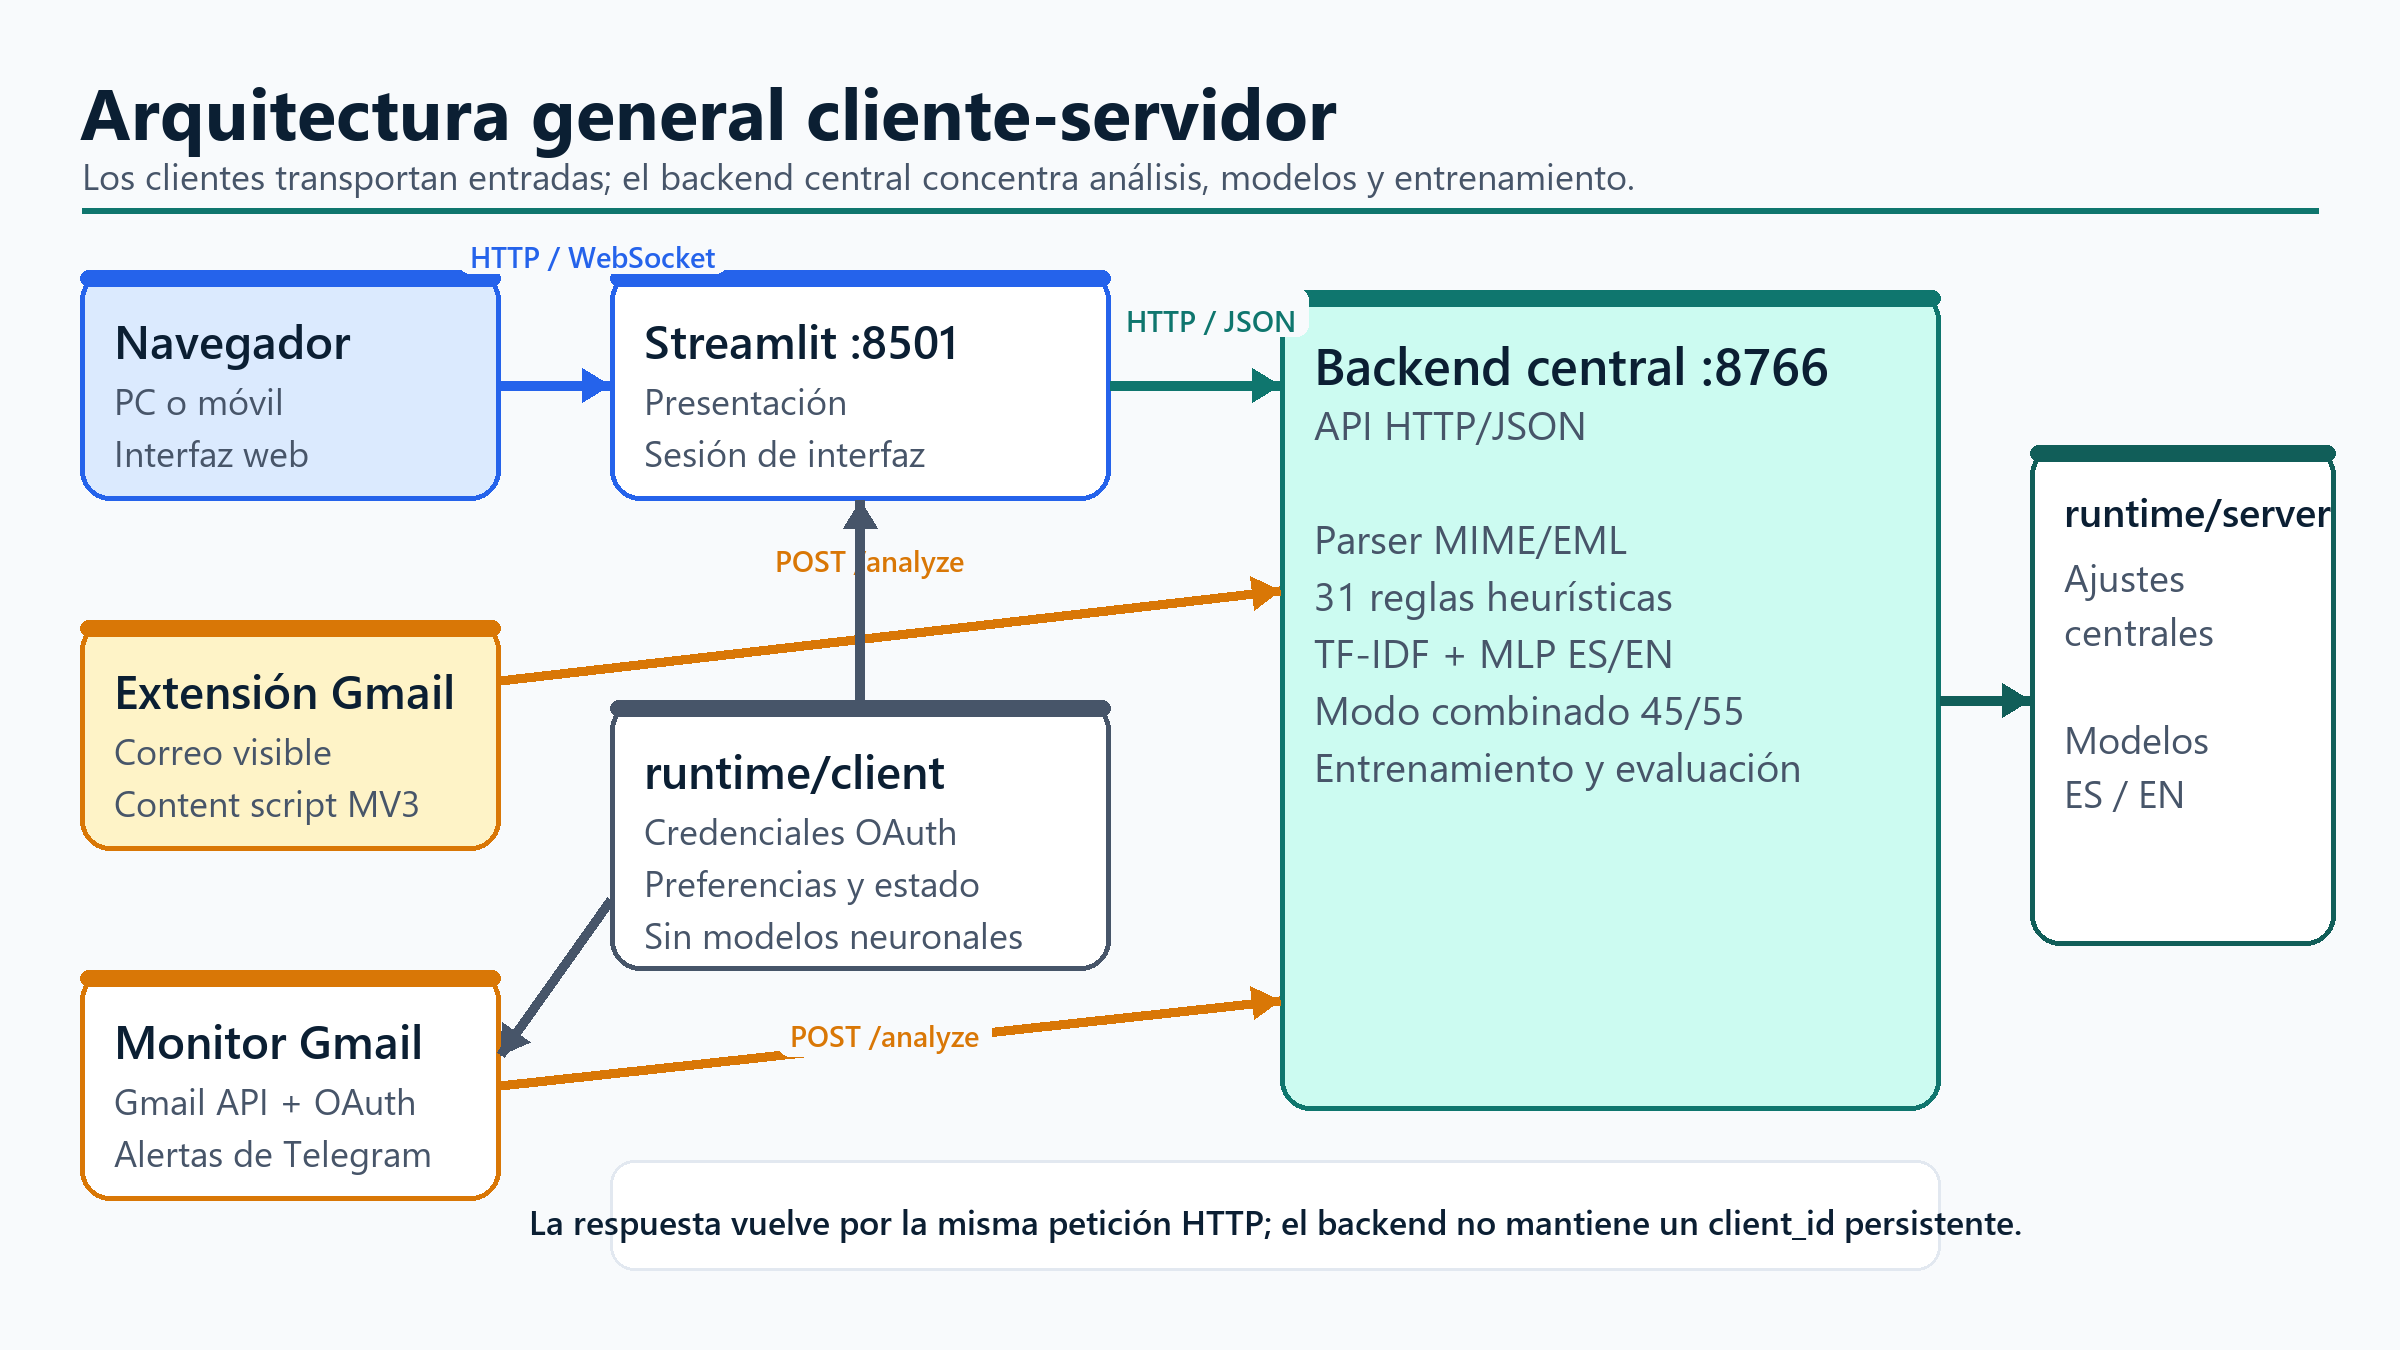
\includegraphics[width=0.92\textwidth]{latex_figures/figura_5_1.png}
  \caption[Arquitectura general cliente-servidor del prototipo.]{Arquitectura general cliente-servidor del prototipo. Fuente: elaboración propia.}
  \label{fig:5-1}
\end{figure}

En cuanto a concurrencia, el backend usa ThreadingHTTPServer y crea un hilo por petición, sin un máximo cerrado en el código. En este equipo se repitieron pruebas de 8 y 16 análisis simultáneos sin fallos; con 16, el percentil 95 de latencia quedó entre 0,58 y 0,66 s, mientras que a 32 aparecieron errores. Por ello se recomiendan 4-8 solicitudes concurrentes para la configuración académica y se presenta 16 solo como máximo comprobado localmente, no como capacidad de producción. Entrenamiento y borrado de modelos se serializan mediante un bloqueo.

A nivel interno, backend\_client.py implementa el transporte común de los clientes y http\_api.py define las rutas, incluidas las operaciones administrativas de ajustes. backend\_service.py concentra análisis, configuración central, datasets, evaluación, entrenamiento, metadatos y activación de versiones. runtime\_paths.py impone las rutas separadas: credenciales, token y estado en runtime/client; configuración y modelos en runtime/server. Dentro del servidor, analysis\_service.py coordina los modos y la caché lingüística; analizador\_email.py normaliza EML; signal\_builder.py, scorer.py y explanations.py construyen el resultado; modelo\_neural.py encapsula TF-IDF + MLP. Las vistas Streamlit no importan almacenamiento de modelos ni ejecutan inferencia.

Las reglas heurísticas se han dividido en módulos especializados: header\_signals.py para cabeceras y autenticación, content\_signals.py para contenido textual y adjuntos, html\_signals.py para estructuras HTML sospechosas y url\_utils.py para extracción y análisis de URLs y dominios. La detección del idioma está centralizada en idioma.py, de modo que la aplicación y la monitorización seleccionan el modelo neuronal con el mismo criterio. Esta división mejora la mantenibilidad y facilita añadir nuevas reglas sin modificar el núcleo del analizador.

\section{Flujo de análisis}

El flujo general comienza con la entrada del correo. Si el usuario sube un archivo .eml, el parser extrae remitente, destinatario, asunto, cuerpo en texto plano, cuerpo HTML, cabeceras, enlaces, anclas y adjuntos. Si el usuario pega el contenido manualmente, se genera una representación simplificada. Cuando la entrada procede de Gmail, la propia aplicación obtiene los mensajes autorizados mediante OAuth y los adapta al mismo formato interno.

A continuación, la entrada se normaliza en una representación interna común (CorreoAnalizado), de modo que las reglas heurísticas no dependen del formato original del mensaje.

Una vez normalizado el correo, SignalBuilder ejecuta 31 reglas y produce un diccionario estable de señales. Además de cabeceras, autenticación, URLs, HTML y adjuntos, incorpora tres patrones bilingües para BEC sin enlace: cambio de datos bancarios, orden urgente de transferencia y suplantación de un directivo bajo aislamiento o confidencialidad. Si el modo lo requiere, el backend detecta el idioma y reutiliza el modelo neuronal central correspondiente.

RiskScorer asigna una ponderación a cada señal activa y calcula una puntuación final entre 0 y 100. Si la puntuación supera el umbral configurado, el mensaje se clasifica como phishing probable. ExplanationBuilder transforma las señales en explicaciones comprensibles. El backend central devuelve ese resultado por HTTP a Streamlit, la extensión o el monitor; los clientes solo lo presentan o, en el caso del monitor, pueden generar una alerta de Telegram y registrar el identificador para evitar duplicados.

\begin{figure}[H]
  \centering
  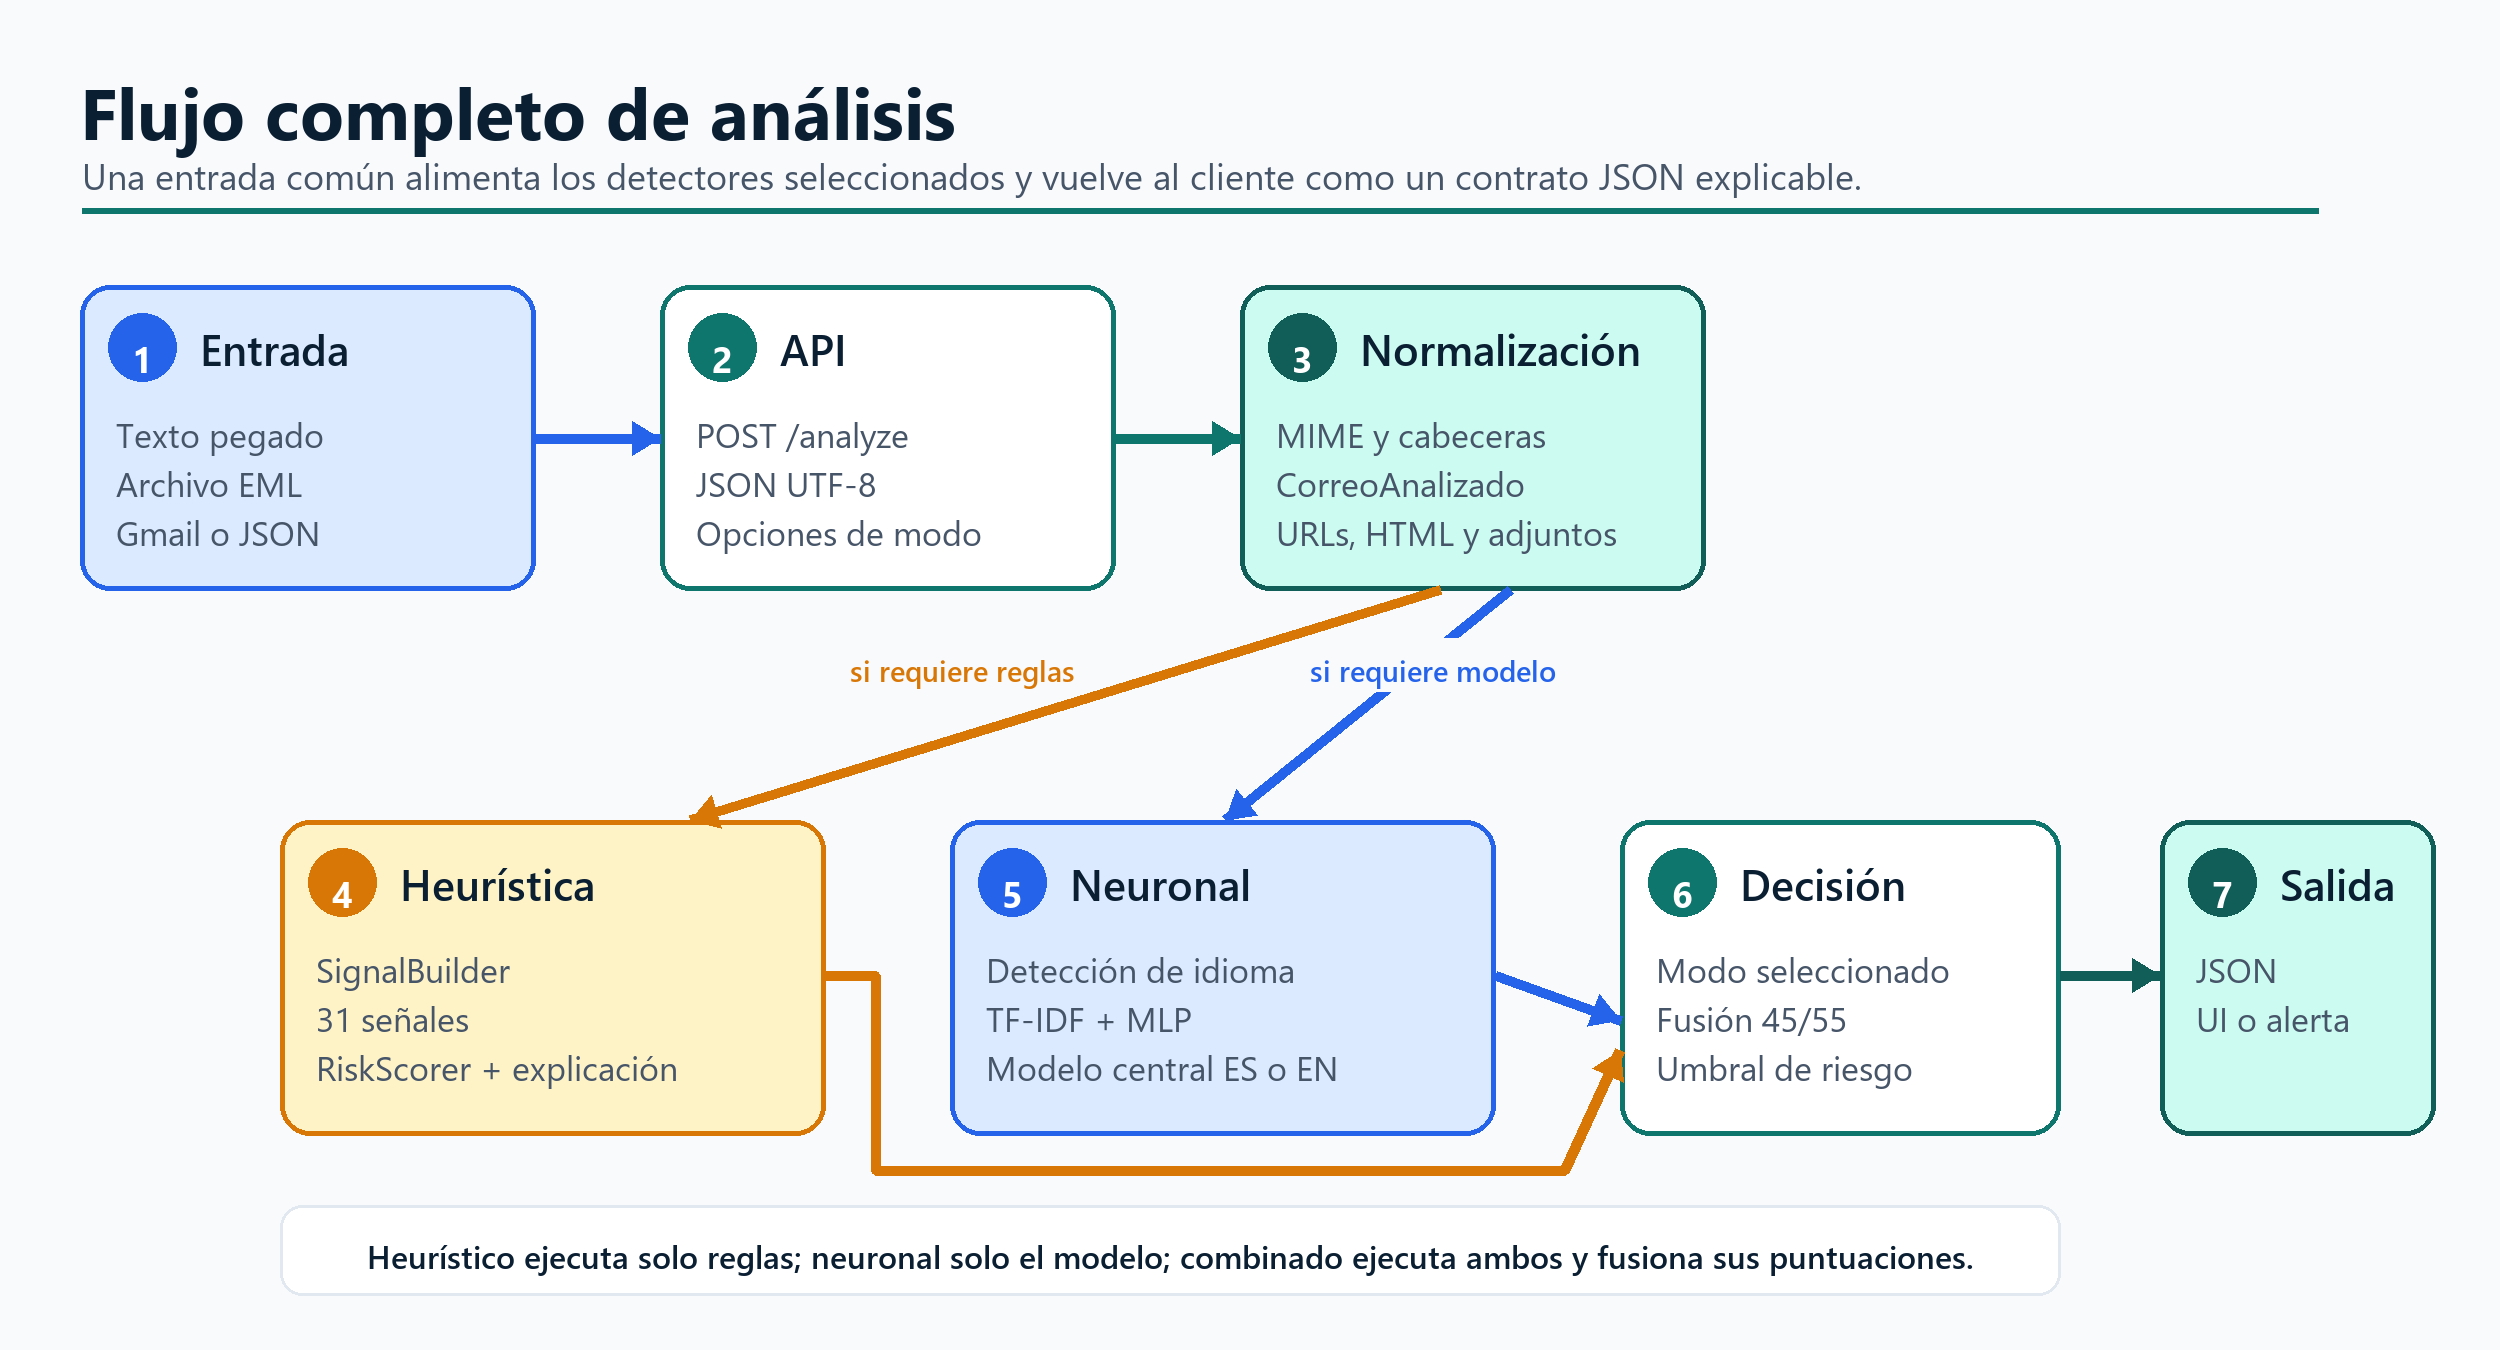
\includegraphics[width=0.92\textwidth]{latex_figures/figura_5_2.png}
  \caption[Flujo de análisis desde la entrada hasta la respuesta del backend.]{Flujo de análisis desde la entrada hasta la respuesta del backend. Fuente: elaboración propia.}
  \label{fig:5-2}
\end{figure}

\section{Sistema heurístico}

El sistema heurístico constituye la parte más explicable del prototipo. Está formado por un conjunto de reglas diseñadas a partir de patrones habituales en correos de phishing. Estas reglas se agrupan en varias categorías.

En primer lugar, se analizan las cabeceras del correo. El sistema interpreta los resultados que los servidores de correo ya han escrito en Received-SPF, Authentication-Results y ARC-Authentication-Results, y detecta estados fail, softfail o errores de SPF, DKIM y DMARC. También revisa incoherencias entre From, Reply-To y Return-Path y si una cabecera DKIM-Signature presente está mal formada. No realiza consultas DNS, no recupera claves públicas y no verifica criptográficamente SPF, DKIM o DMARC; por tanto, es una interpretación pasiva de cabeceras, no una validación completa de autenticación.

En segundo lugar, se analizan los enlaces. El sistema extrae URLs del texto y del HTML, comprueba la presencia de dominios en listas negras locales, detecta acortadores conocidos, identifica dominios con punycode o caracteres Unicode, y revisa parámetros de redirección sospechosos.

En tercer lugar, se estudia el contenido HTML. Se detectan formularios con acciones vacías, relativas o dirigidas a dominios sospechosos, así como elementos como iframe, base href, enlaces javascript: o redirecciones mediante meta refresh.

Por último, se analizan rasgos de ingeniería social presentes en el texto, como saludos genéricos, lenguaje urgente, asuntos sospechosos, solicitudes de credenciales o referencias a documentos adjuntos.

\section{Clasificador neuronal}

Además del sistema heurístico, se ha implementado un clasificador neuronal basado en scikit-learn. El modelo utiliza un pipeline formado por un vectorizador TF-IDF y un MLPClassifier. Los hiperparámetros están centralizados en HiperparametrosModelo y sus valores predeterminados se persisten en runtime/server/.env.local. La interfaz los consulta y modifica mediante la API administrativa; un cliente puede enviar una excepción explícita al comparar o entrenar, pero no escribe el sistema de archivos del servidor.

El sistema permite una versión activa en español y otra en inglés. La vista de entrenamiento serializa los CSV y, solo cuando se solicita una excepción, los hiperparámetros; de lo contrario, el backend usa sus valores centrales persistidos. El servidor valida datos, entrena desde cero, guarda el artefacto de forma atómica en runtime/server/models e invalida la caché. Evaluación y comparación también se ejecutan en el servidor; los clientes reciben únicamente métricas y metadatos.

Los modelos entrenados se almacenan mediante joblib en runtime/server/models, diferenciando el artefacto español del inglés. Solo el backend accede a esas rutas. Durante el análisis, el servidor detecta el idioma con langdetect y reutiliza un detector cacheado por idioma. Si el modelo esperado no existe, está corrupto o tiene metadatos incompatibles, se entrena un modelo sintético del mismo idioma; nunca se reutiliza silenciosamente el modelo de la lengua opuesta.

La configuración final usa unigramas y bigramas, limita el vocabulario y mantiene una red compacta. La tabla recoge los valores efectivos de ambos modelos; las stopwords son las de scikit-learn para inglés y una lista local versionada para español.

\begingroup
  \arrayrulecolor{uemcgreen}
\begin{table}[H]
  \centering
  \small
  \caption{Hiperparámetros finales del pipeline TF-IDF + MLP.}
  \label{tab:5-3}
  \begin{tabularx}{\textwidth}{|X|X|X|}
    \hline
    \rowcolor{uemcgreen}
    \textcolor{white}{\textbf{Componente}} & \textcolor{white}{\textbf{Parámetro}} & \textcolor{white}{\textbf{Valor final}} \\
    \hline
    TF-IDF & ngram\_range & (1, 2) \\
    \hline
    \rowcolor{tablelight}
    TF-IDF & max\_features & 3.000 \\
    \hline
    TF-IDF & min\_df & 1 \\
    \hline
    \rowcolor{tablelight}
    TF-IDF & strip\_accents / stopwords & unicode / inglés incorporadas o español local \\
    \hline
    MLP & hidden\_layer\_sizes & (64, 32) \\
    \hline
    \rowcolor{tablelight}
    MLP & activation & relu \\
    \hline
    MLP & alpha / learning\_rate\_init & 0,0001 / 0,001 \\
    \hline
    \rowcolor{tablelight}
    MLP & max\_iter / early\_stopping & 500 / False \\
    \hline
    MLP & random\_state & 42 \\
    \hline
  \end{tabularx}
\end{table}
\endgroup

Los artefactos activos se entrenaron el 30 de agosto de 2026: ES con 1.148 muestras (SHA-256 \nolinkurl{165e7c2bf292adf1d7bc88d936b3c14f4c7fe8f1caa3d2615718ca1190aaefb0}) y EN con 65.661 (SHA-256 \nolinkurl{a3dd9dc3216445c70574982ad7b2515e02830e1a8c0f2ad841cf2c2eb2c56d69}). Los hashes permiten comprobar exactamente qué ficheros se utilizaron en la entrega.

\section{Interfaz de usuario}

El cliente web se desarrolla con Streamlit y organiza cinco vistas: Inicio, Configuración, Detección, Monitor y Entrenamiento. Comparte un sistema visual adaptable con cabecera de marca, navegación compacta, tarjetas de estado y componentes coherentes. Detección ordena fuente, configuración y resultado en tres pasos; Configuración agrupa conexiones, monitor, backend y red neuronal en pestañas. Sus responsabilidades son recoger entradas, llamar mediante BackendClient y presentar la respuesta, sin cargar modelos ni exponer rutas locales completas de credenciales.

El resultado se muestra mediante una puntuación de riesgo, una clasificación global y un panel de detalles. En el análisis heurístico, el usuario puede consultar qué señales se han activado y leer una explicación de cada una. Esta decisión busca mejorar la transparencia del sistema, evitando que el resultado sea una simple etiqueta opaca.

La integración con Gmail usa OAuth de solo lectura. La vista de detección obtiene EML autorizados y los remite al backend; el proceso monitor\_gmail.py hace lo mismo periódicamente y puede notificar por Telegram. Ambos consumen la misma versión central y un fallo temporal queda controlado para reintento.

\section{Diseño modular}

Durante el desarrollo se ha realizado una refactorización orientada a SOLID y a una frontera cliente-servidor explícita. La presentación depende de BackendClient; el servidor separa transporte, casos de uso, señales, puntuación, explicaciones, datasets y aprendizaje. El almacenamiento sigue la misma frontera: runtime/client contiene secretos y preferencias propios de cada instalación, mientras runtime/server contiene configuración y modelos centrales. Así, los detalles del modelo permanecen fuera de Streamlit, extensión y monitor.

Esta organización permite que cada módulo tenga una responsabilidad principal. Por ejemplo, SignalBuilder no calcula puntuaciones, sino que únicamente construye señales; RiskScorer no conoce cómo se han obtenido las señales, solo calcula el riesgo; y ExplanationBuilder no decide si un correo es phishing, sino que transforma resultados técnicos en texto comprensible.

\begingroup
  \arrayrulecolor{uemcgreen}
\begin{table}[H]
  \centering
  \small
  \caption{Capas y responsabilidades del diseño modular.}
  \label{tab:5-4}
  \begin{tabularx}{\textwidth}{|X|X|X|}
    \hline
    \rowcolor{uemcgreen}
    \textcolor{white}{\textbf{Capa}} & \textcolor{white}{\textbf{Módulos principales}} & \textcolor{white}{\textbf{Responsabilidad}} \\
    \hline
    Presentación y clientes & app.py, detect\_app.py, config\_app.py, train\_app.py, monitor\_app.py y extension\_gmail/ & Recoger entradas, mantener el estado visual y presentar la respuesta del backend. \\
    \hline
    \rowcolor{tablelight}
    Transporte & backend\_client.py y http\_api.py & Serializar JSON, aplicar límites, gestionar CORS/autorización y devolver códigos HTTP. \\
    \hline
    Aplicación & backend\_service.py y analysis\_service.py & Coordinar análisis, modos, caché, ajustes, entrenamiento, evaluación y versiones. \\
    \hline
    \rowcolor{tablelight}
    Dominio de análisis & analizador\_email.py, correo.py, signal\_builder.py, scorer.py y explanations.py & Normalizar el correo, construir señales, calcular el riesgo y generar explicaciones. \\
    \hline
    Aprendizaje y datos & modelo\_neural.py, model\_config.py, dataset.py, training\_protocol.py y metrics.py & Vectorizar, entrenar, inferir, limpiar datasets y calcular métricas reproducibles. \\
    \hline
    \rowcolor{tablelight}
    Infraestructura e integraciones & runtime\_paths.py, env\_loader.py, file\_utils.py, gmail\_client.py y telegram\_notifier.py & Separar persistencia, escribir de forma atómica e integrar Gmail y Telegram. \\
    \hline
  \end{tabularx}
\end{table}
\endgroup

Esta separación facilita la evolución del prototipo. Pueden añadirse reglas o sustituirse el clasificador en el servidor sin redistribuir los clientes. La versión revisada ejecuta correctamente 94 pruebas Python y 2 recorridos reales con Chromium; GitHub Actions repite pruebas, Ruff, calibración, evaluación reproducible, respaldo de defensa y navegación de interfaz.

\section{Modelos UML del diseño final}
\label{sec:uml}

Estos cinco modelos UML documentan el diseño final mediante casos de uso, clases, secuencia, componentes y despliegue. Se han completado durante la revisión a partir del código y no se presentan como documentos anteriores a la implementación. Se omiten métodos auxiliares para facilitar la lectura.

\subsection{Casos de uso}
El usuario analiza mensajes y consulta sus explicaciones. El responsable configura la instalación y administra modelos. Son funciones de uso, no cuentas aisladas: el prototipo comparte configuración y utiliza un token administrativo. El monitor lee Gmail mediante OAuth y puede enviar alertas a Telegram.

\begin{figure}[H]
\centering
\begin{tikzpicture}[x=1cm,y=0.82cm,font=\small,
 usecase/.style={ellipse,draw=uemcgreen,fill=tablelight,align=center,minimum width=4.2cm,minimum height=1cm},
 actor/.style={draw=uemcgreen,fill=white,align=center,font=\small\bfseries},link/.style={draw=uemcgreen}]
\draw[draw=uemcgreen] (3,0) rectangle (12,10.6);
\node[anchor=north,font=\bfseries] at (7.5,10.4) {Sistema de detección};
\node[actor] (user) at (1.1,8.9) {\guillemotleft actor\guillemotright\\Usuario};
\node[actor] (admin) at (1.1,3.8) {\guillemotleft actor\guillemotright\\Responsable\\de instalación};
\node[actor] (gmail) at (13.3,8.9) {\guillemotleft actor\guillemotright\\Gmail};
\node[actor] (telegram) at (13.3,1.1) {\guillemotleft actor\guillemotright\\Telegram};
\node[usecase] (analyze) at (7.4,8.9) {Analizar texto, EML\\o mensaje de Gmail};
\node[usecase] (explain) at (7.4,7.1) {Consultar riesgo\\y explicación};
\node[usecase] (settings) at (7.4,5.5) {Configurar conexión\\y parámetros};
\node[usecase] (models) at (7.4,3.8) {Entrenar, evaluar\\o eliminar un modelo};
\node[usecase] (monitor) at (7.4,2.2) {Monitorizar mensajes};
\node[usecase] (alert) at (7.4,0.7) {Enviar alerta};
\draw[link] (user)--(analyze);\draw[link] (user)--(explain);
\draw[link] (admin)--(settings);\draw[link] (admin)--(models);\draw[link] (admin)--(monitor);
\draw[link] (gmail)--(analyze);\draw[link] (gmail) |- (monitor);
\draw[link] (telegram)--(alert);
\draw[dashed,-{Stealth},draw=uemcgreen] (alert)--node[right,font=\scriptsize]{\guillemotleft extend\guillemotright}(monitor);
\end{tikzpicture}
\caption{Casos de uso principales. La alerta extiende la monitorización cuando se cumple la condición configurada. Fuente: elaboración propia.}
\label{fig:uml-casos}
\end{figure}

El análisis requiere un backend disponible. Tras elegir entrada y modo, se valida y normaliza el mensaje y se devuelven riesgo, veredicto y explicación. Las entradas inválidas o los fallos de conexión se comunican sin ejecutar un detector local alternativo. La administración exige autorización cuando hay un token configurado; el entrenamiento activa la versión después del ajuste y la escritura del artefacto.

\clearpage
\subsection{Clases y responsabilidades}
\begin{figure}[H]
\centering
\begin{tikzpicture}[font=\scriptsize, x=1cm,y=1cm,
 cls/.style={rectangle split,rectangle split parts=3,draw=uemcgreen,fill=tablelight,align=left,text width=5.8cm,inner sep=5pt},
 dep/.style={dashed,-{Stealth},draw=uemcgreen},assoc/.style={-{Stealth},draw=uemcgreen}]
\node[cls] (client) at (0,0) {\textbf{BackendClient}\nodepart{second}base\_url; admin\_token\nodepart{third}+ analyze(); train(); evaluate()\\+ settings(); delete\_model()};
\node[cls] (backend) at (7.2,0) {\textbf{AnalysisBackendService}\nodepart{second}config; \_service; \_training\_lock\nodepart{third}+ analyze\_payload(); train\_payload()\\+ update\_settings\_payload()};
\node[cls] (service) at (7.2,-3.2) {\textbf{EmailAnalysisService}\nodepart{second}config; \_detectores[idioma]\nodepart{third}+ analyze\_all(); analyze\_heuristic()\\+ analyze\_neural(); invalidate\_detector()};
\node[cls] (analyzer) at (0,-3.2) {\textbf{PhishingAnalyzer}\nodepart{second}correo; signal\_builder; explanation\_builder\nodepart{third}+ analyze()};
\node[cls] (detector) at (7.2,-6.4) {\textbf{NeuralPhishingDetector}\nodepart{second}classifier; source\nodepart{third}+ analyze(texto, remitente, subject)};
\node[cls] (classifier) at (0,-6.4) {\textbf{NeuralPhishingClassifier}\nodepart{second}pipeline; last\_training\_stats\nodepart{third}+ fit(); predict(); predict\_proba()\\+ save(); load()};
\node[cls] (storage) at (0,-9.6) {\textbf{ModelStorage}\nodepart{second}path\nodepart{third}+ load(); save(); exists()};
\node[cls] (trainer) at (7.2,-9.6) {\textbf{NeuralModelTrainer}\nodepart{second}storage\nodepart{third}+ train\_from\_csvs(); save()};
\draw[dep] (client.north) -- ++(0,0.65) -| node[pos=0.25,above]{HTTP/JSON; sin referencia local} (backend.north);
\draw[{Diamond[length=6pt]}-] (backend)--node[right]{1}(service);
\draw[dep] (service.south) -- ++(0,-0.45) -| node[pos=0.25,below]{fachada heurística} (analyzer.south);
\draw[assoc] (service)--node[right]{0..2 en caché}(detector);
\draw[assoc] (detector)--node[above]{1}(classifier);
\draw[dep] (storage)--node[left]{carga/guarda}(classifier);
\draw[assoc] (trainer)--node[above]{1}(storage);
\draw[dep] (backend.east) -- ++(0.55,0) |- (trainer.east);
\end{tikzpicture}
\caption{Clases principales y relaciones del análisis y aprendizaje. Rombo lleno: composición; línea continua: asociación; línea discontinua: dependencia. La relación entre cliente y servicio atraviesa la API. Fuente: elaboración propia.}
\label{fig:uml-clases}
\end{figure}

\nolinkurl{AnalysisBackendConfig} suministra modo, umbral, pesos y rutas al servicio. \nolinkurl{HiperparametrosModelo} describe el vectorizador y el MLP. El analizador heurístico delega la construcción de señales en \nolinkurl{SignalBuilder}, la puntuación en \nolinkurl{RiskScorer} y el texto explicativo en \nolinkurl{ExplanationBuilder}. \nolinkurl{ModelStorage} persiste el clasificador; la activación administrativa utiliza escritura atómica y la invalidación de la caché en el servicio. Estas dependencias separan el transporte, la lógica de aplicación y el aprendizaje.

\clearpage
\subsection{Secuencia de análisis combinado}
La figura~\ref{fig:uml-secuencia} representa una petición válida en modo combinado. La normalización sucede antes de la inferencia. En este modo se obtienen ambos resultados y se aplica la política de fusión. El detector lingüístico selecciona el modelo ES o EN; la caché evita recargarlo en cada petición. La figura agrupa la API y su handler en la misma línea de vida para facilitar la lectura.

\begin{figure}[H]
\centering
\begin{tikzpicture}[x=1cm,y=1cm,font=\scriptsize,
 life/.style={draw=uemcgreen,fill=tablelight,align=center,minimum width=2.5cm,minimum height=0.85cm},
 msg/.style={-{Stealth},draw=uemcgreen},ret/.style={dashed,-{Stealth},draw=uemcgreen}]
\foreach \x/\id/\name in {0/ui/Streamlit y cliente,3.6/api/API y servicio backend,7.2/svc/EmailAnalysisService,10.8/det/Detectores}{
\node[life] (\id) at (\x,0) {\name};
\draw[dashed,gray] (\x,-0.45)--(\x,-11.8);}
\draw[msg] (0,-1)--node[above]{POST /analyze: entrada y opciones}(3.6,-1);
\draw[msg] (3.6,-1.8)--(4.25,-1.8)--(4.25,-2.45)--node[below,align=center]{validar entrada y normalizar}(3.6,-2.45);
\draw[msg] (3.6,-3.2)--node[above]{analyze\_all(datos)}(7.2,-3.2);
\draw[msg] (7.2,-4)--node[above]{análisis heurístico}(10.8,-4);
\draw[ret] (10.8,-4.75)--node[above]{señales, riesgo, explicación}(7.2,-4.75);
\draw[msg] (7.2,-5.5)--(7.8,-5.5)--(7.8,-6.15)--node[below,align=center]{idioma y caché ES/EN}(7.2,-6.15);
\draw[msg] (7.2,-7)--node[above]{análisis neuronal}(10.8,-7);
\draw[ret] (10.8,-7.75)--node[above]{puntuación neuronal}(7.2,-7.75);
\draw[ret] (7.2,-8.6)--node[above]{resultados de ambos detectores}(3.6,-8.6);
\draw[msg] (3.6,-9.3)--(4.25,-9.3)--(4.25,-10)--node[below,align=center]{fusión, umbral y metadatos}(3.6,-10);
\draw[ret] (3.6,-11)--node[above]{HTTP 200: resultado JSON}(0,-11);
\node[anchor=north,align=center] at (0,-11.3) {mostrar veredicto\ y explicación};
\end{tikzpicture}
\caption{Secuencia de una petición válida de análisis combinado. Fuente: elaboración propia.}
\label{fig:uml-secuencia}
\end{figure}

Si el JSON, el tipo de contenido o los campos no son válidos, el handler devuelve HTTP 400 sin completar el análisis. Una excepción interna devuelve HTTP 500 con un mensaje genérico. El cliente distingue errores de servicio e indisponibilidad. Para entrenar, la secuencia cambia después de la autorización: validar CSV y parámetros, adquirir el bloqueo, entrenar, guardar atómicamente, invalidar cachés y devolver metadatos. Evaluar y comparar no sustituyen por sí solos el modelo activo.

\clearpage
\subsection{Componentes}
\begin{figure}[H]
\centering
\begin{tikzpicture}[x=0.95cm,y=1cm,font=\small,
 comp/.style={draw=uemcgreen,fill=tablelight,rectangle,align=center,text width=3.8cm,minimum height=1.2cm},
 dep/.style={dashed,-{Stealth},draw=uemcgreen}]
\node[comp] (web) at (0,0) {\guillemotleft component\guillemotright\\Streamlit y BackendClient};
\node[comp] (ext) at (5,0) {\guillemotleft component\guillemotright\\Extensión Gmail};
\node[comp] (mon) at (10,0) {\guillemotleft component\guillemotright\\Monitor Gmail};
\node[comp,text width=6cm] (api) at (5,-2.8) {\guillemotleft component\guillemotright\\API HTTP y servicios de aplicación};
\node[comp] (parser) at (0,-5.5) {\guillemotleft component\guillemotright\\Normalización MIME/EML};
\node[comp] (rules) at (5,-5.5) {\guillemotleft component\guillemotright\\Reglas y explicaciones};
\node[comp] (ml) at (10,-5.5) {\guillemotleft component\guillemotright\\Aprendizaje TF-IDF + MLP};
\node[comp,text width=5.4cm] (storage) at (10,-8.3) {\guillemotleft artifact\guillemotright\\Configuración y modelos ES/EN};
\node[comp,text width=4.5cm] (external) at (0,-8.3) {\guillemotleft external service\guillemotright\\Gmail API y Telegram API};
\draw[dep] (web)--node[left]{HTTP/JSON}(api);
\draw[dep] (ext)--node[right]{HTTP/JSON}(api);
\draw[dep] (mon)--node[right]{HTTP/JSON}(api);
\draw[dep] (api)--(parser);\draw[dep] (api)--(rules);\draw[dep] (api)--(ml);
\draw[dep] (ml)--(storage);
\draw[dep] (api.east) -- (13.7,-2.8) |- (storage.east);
\draw[dep] (mon.east) -- (13.3,0) -- (13.3,-10) -| (external.south);
\draw[dep] (web.west) -- (-2.8,0) -- (-2.8,-8.3) -- (external.west);
\end{tikzpicture}
\caption{Vista de componentes y dependencias. Los servicios externos son consumidos por clientes autorizados; el motor de análisis no consulta reputación online. Fuente: elaboración propia.}
\label{fig:uml-componentes}
\end{figure}

La API ofrece análisis y operaciones administrativas sobre datasets, parámetros y modelos. El contenido del correo se normaliza en el servidor; la extracción del mensaje visible en la extensión es una entrada parcial procedente del DOM. Gmail OAuth y Telegram son integraciones de los clientes y del monitor. El proxy opcional de compatibilidad en el puerto 8767 solo reenvía peticiones al backend; no aloja modelos ni constituye un segundo motor de detección.

\clearpage
\subsection{Despliegue y persistencia}
\begin{figure}[H]
\centering
\begin{tikzpicture}[x=1cm,y=0.78cm,font=\small,
 nodebox/.style={draw=uemcgreen,fill=tablelight,align=center,text width=5.2cm,minimum height=1.3cm},
 wire/.style={-{Stealth},draw=uemcgreen}]
\draw[draw=uemcgreen,thick] (-3.2,1.3) rectangle (11,-10.2);
\node[anchor=north west,font=\bfseries] at (-3,1.15) {\guillemotleft device\guillemotright\ Equipo de demostración};
\node[nodebox] (browser) at (0,-0.7) {\guillemotleft executionEnvironment\guillemotright\\Navegador y extensión Gmail};
\node[nodebox] (web) at (0,-3.5) {\guillemotleft executionEnvironment\guillemotright\\Streamlit :8501};
\node[nodebox] (backend) at (7.5,-3.5) {\guillemotleft executionEnvironment\guillemotright\\Backend :8766};
\node[nodebox] (monitor) at (7.5,-0.7) {\guillemotleft executionEnvironment\guillemotright\\Proceso monitor Gmail};
\node[nodebox] (clientfiles) at (0,-7) {\guillemotleft artifact\guillemotright\\runtime/client/\\OAuth, preferencias y estado};
\node[nodebox] (serverfiles) at (7.5,-7) {\guillemotleft artifact\guillemotright\\runtime/server/\\Configuración y modelos ES/EN};
\draw[wire] (browser)--node[left]{interfaz web}(web);
\draw[wire] (web)--node[above]{HTTP/JSON}(backend);
\draw[wire] (monitor)--node[right]{HTTP/JSON}(backend);
\draw[wire] (browser.north) -- ++(0,0.6) -| node[pos=0.35,above,font=\scriptsize]{extensión: HTTP/JSON directo} (backend.east);
\draw[dashed,draw=uemcgreen] (web)--(clientfiles);
\draw[dashed,draw=uemcgreen] (backend)--(serverfiles);
\draw[dashed,draw=uemcgreen] (monitor.east) -- ++(0.5,0) |- (0,-9) -- (clientfiles.south);
\node[align=center,text width=11.5cm] at (3.8,-11.2) {\guillemotleft external service\guillemotright\ Gmail y Telegram\\Conexiones HTTPS de los clientes autorizados fuera del equipo local.};
\end{tikzpicture}
\caption{Despliegue local de referencia y propiedad de los datos persistentes. Fuente: elaboración propia.}
\label{fig:uml-despliegue}
\end{figure}

El backend escucha por defecto en \nolinkurl{127.0.0.1:8766}. La separación entre cliente y servidor es lógica y de procesos, aunque compartan equipo. Cuando se muestra la web en una LAN, puede exponerse únicamente Streamlit y conservar el backend en loopback. Las credenciales persistentes pertenecen a la instalación cliente, no a usuarios web aislados. La exposición remota del backend exige una decisión explícita, token administrativo y controles adicionales; no se presenta como despliegue de producción.


\section{Limitaciones}

Las listas negras son locales: no se consultan servicios de reputación en tiempo real ni se analiza dinámicamente el destino de los enlaces. Tampoco se validan certificados digitales ni se comprueba la reputación histórica de los dominios. Streamlit se utiliza en un entorno académico controlado, sin gestión multiusuario, control de acceso ni aislamiento de datos para un despliegue público.

El modelo neuronal depende de la calidad y representatividad de los datos de entrenamiento. Aunque admite CSV externos, su rendimiento requiere evaluación con conjuntos amplios, recientes y equilibrados. No incorpora transformers ni LLMs, identificados en el estado del arte como líneas futuras junto con la detección semántica de principios de ingeniería social.

\chapter{Pruebas, resultados y discusión}

\section{Pruebas unitarias y de integración}

La versión revisada ejecuta 94 pruebas unitarias y de integración mediante unittest. Cubren EML, señales BEC, combinación calibrada, selección determinista de idioma, cliente HTTP, entrenamiento central, Gmail, monitor, heurísticas, clasificador, persistencia separada, ajustes por API, autenticación administrativa, extensión, evaluación externa, respaldo de defensa y Telegram. Una prueba integral recorre Gmail EML, JSON, HTTP, backend, estado y alerta Telegram. Además, 2 pruebas con Chromium recorren la extensión y un análisis real entre Streamlit y backend. Todas finalizaron correctamente; los avisos de convergencia proceden de iteraciones reducidas del MLP en pruebas rápidas.

\section{Rendimiento y eficiencia de arranque}

Para cuantificar el coste operativo se añadió un benchmark reproducible que mide el arranque, el análisis heurístico, la detección de idioma, la carga de modelos y la inferencia. Cada microbenchmark se ejecutó con cinco repeticiones y se tomó la mediana por operación; las importaciones se midieron en procesos nuevos para evitar que la caché de módulos ocultase el coste de inicio.

\subsection{Entorno de ejecución medido}

Las cifras se obtuvieron en Windows 11 Home 25H2 de 64 bits (compilación 26200.9278), con AMD Ryzen 7 7800X3D de 8 núcleos y 16 hilos y 63,1 GiB de RAM física. El entorno utilizó Python 3.12.7, scikit-learn 1.9.0, Streamlit 1.58.0, NumPy 2.4.6, SciPy 1.17.1 y joblib 1.5.3. requirements.txt y constraints.txt fijan estas versiones para repetir la prueba.

El perfilado localizó el principal cuello de botella en las importaciones anticipadas. Importar únicamente las heurísticas requería 1098,5090 ms y, tras diferir la carga de scikit-learn y del subsistema neuronal, pasó a 37,0194 ms: una reducción del 96,6 \% y una aceleración de 29,7 veces. El arranque frío de la aplicación Streamlit bajó de 1326,5726 ms a 315,1490 ms, una mejora del 76,2 \% y 4,2 veces.

Las rutas de inferencia permanecieron estables: el análisis heurístico pasó de 0,1097 ms a 0,1084 ms, la detección de idioma de 2,8185 ms a 2,8230 ms, la predicción neuronal de 0,3101 ms a 0,3190 ms y el análisis combinado en caliente de 3,4187 ms a 3,3611 ms. Las variaciones de hasta el 3 \% se consideran ruido de medición, ya que no se modificaron reglas, pesos ni modelos.

\section{Diseño experimental y datasets}

El protocolo reproducible fija fuentes, licencias y SHA-256 sin versionar mensajes. En español combina el entrenamiento de Softecapps (2024), con DOI 10.57967/hf/2264, y SMS Spam Mexico (Iván, 2026): tras eliminar duplicados, conflictos y una coincidencia con el test quedan 1.148 textos, mientras 209 del split oficial se reservan para prueba. En inglés usa el agregado descrito por Al-Subaiey et al. (2024), que reúne CEAS, Enron, Ling, Nazario, Nigerian Fraud y SpamAssassin; no añade de nuevo sus componentes. Tras retirar 408 duplicados quedan 82.077 textos, divididos de forma estratificada 80/20 con semilla 42. Los joblib guardan el pipeline y metadatos, nunca el texto bruto.

\begingroup
  \arrayrulecolor{uemcgreen}
\begin{table}[H]
  \centering
  \small
  \caption{Conjuntos empleados y separación experimental.}
  \label{tab:6-1}
  \begin{tabularx}{\textwidth}{|X|X|X|X|X|X|}
    \hline
    \rowcolor{uemcgreen}
    \textcolor{white}{\textbf{Conjunto}} & \textcolor{white}{\textbf{N}} & \textcolor{white}{\textbf{Clase positiva (1)}} & \textcolor{white}{\textbf{Clase negativa (0)}} & \textcolor{white}{\textbf{Procedencia}} & \textcolor{white}{\textbf{Uso}} \\
    \hline
    Entrena\-miento ES & 1.148 & 613 & 535 & Hugging Face + SMS Spam Mexico & Ajuste del modelo español \\
    \hline
    \rowcolor{tablelight}
    Prueba ES & 209 & 100 & 109 & Split oficial softecapps & Holdout español \\
    \hline
    Entrena\-miento EN & 65.661 & 34.275 & 31.386 & 80 \% del agregado deduplicado & Ajuste del modelo inglés \\
    \hline
    \rowcolor{tablelight}
    Prueba EN & 16.416 & 8.569 & 7.847 & 20 \% estratificado del agregado & Holdout inglés \\
    \hline
    Calibración & 40 & 20 & 20 & Casos sintéticos ES/EN; 10 por idioma y clase & Cinco particiones para pesos y umbral \\
    \hline
    \rowcolor{tablelight}
    Evaluación EML & 16 & 8 & 8 & EML sintéticos reservados; 4 por idioma y clase & Comparación final de los tres modos \\
    \hline
    Validación Zenodo & 100 & 23 & 77 & 100 textos únicos de 2.000 filas & Diagnóstico secundario \\
    \hline
    \rowcolor{tablelight}
    DIFrauD & 1.528 & 608 & 920 & Split público histórico de phishing & Diagnóstico externo con riesgo de solapamiento \\
    \hline
  \end{tabularx}
\end{table}
\endgroup

La separación se realiza antes del ajuste. Español conserva el test oficial sin coincidencias exactas e inglés deduplica antes de dividir. Otros 40 casos sintéticos y bilingües calibran la fusión mediante cinco particiones; 16 EML distintos prueban después los tres modos con MIME y cabeceras. La validación secundaria emplea una muestra única del conjunto de Miltchev et al. (2024) y DIFrauD; este último no se considera independiente por posible solapamiento de fuentes históricas con el agregado inglés (Boumber et al., 2024).

evaluation/training\_sources.json fija las URLs, licencias y huellas de los CSV; scripts/retrain\_reproducible.py verifica, divide, entrena y evalúa. Los campos históricos llamados phishing/legitimate representan en realidad clase positiva (1) y negativa (0): los corpus ES son spam/ham usados como proxy de smishing/phishing y la clase positiva EN mezcla phishing y spam. No se equiparan semánticamente spam y phishing. Los holdouts de texto, además, carecen de MIME; estas limitaciones impiden extrapolar las cifras a producción.

\section{Resultados comparados}

La calibración recorre 40 casos separados del entrenamiento y de la evaluación final, en cinco particiones estratificadas por idioma y etiqueta. Prueba pesos heurísticos del 20 \% al 50 \% en pasos de 5 (el resto es neuronal), umbrales del 20 al 60 en pasos de 1 y alta confianza del 65 al 85 en pasos de 5. Ordena por la menor accuracy balanceada entre particiones, su media y el valor global; después usa F1, recall y precisión. Los desempates predefinidos prefieren umbral cercano a 45, alta confianza cercana a 70 y mayor peso neuronal.

La combinación seleccionada fue 45 \% heurístico, 55 \% neuronal, umbral 21 y alta confianza 70: obtuvo 0,625 de accuracy balanceada mínima entre particiones, 0,825 de media/global, F1 0,8293, recall 0,85 y precisión 0,8095. El reparto 50/50 empató en métricas y perdió por el desempate declarado. El umbral 21 se optimizó para el combinado y se conserva como política común configurable; la puntuación resultante no es una probabilidad calibrada.

\begingroup
  \arrayrulecolor{uemcgreen}
\begin{table}[H]
  \centering
  \small
  \caption{Métricas sobre los holdouts de texto.}
  \label{tab:6-2}
  \begin{tabularx}{\textwidth}{|X|X|X|X|X|X|}
    \hline
    \rowcolor{uemcgreen}
    \textcolor{white}{\textbf{Idioma/modo}} & \textcolor{white}{\textbf{N}} & \textcolor{white}{\textbf{Accuracy}} & \textcolor{white}{\textbf{Precisión}} & \textcolor{white}{\textbf{Recall}} & \textcolor{white}{\textbf{F1}} \\
    \hline
    ES heurístico & 209 & 52,2 \% & 0,0 \% & 0,0 \% & 0,0 \% \\
    \hline
    \rowcolor{tablelight}
    ES neuronal & 209 & 87,1 \% & 82,9 \% & 92,0 \% & 87,2 \% \\
    \hline
    ES combinado & 209 & 89,5 \% & 87,5 \% & 91,0 \% & 89,2 \% \\
    \hline
    \rowcolor{tablelight}
    EN heurístico & 16.416 & 48,0 \% & 92,7 \% & 0,4 \% & 0,9 \% \\
    \hline
    EN neuronal & 16.416 & 98,3 \% & 98,0 \% & 98,8 \% & 98,4 \% \\
    \hline
    \rowcolor{tablelight}
    EN combinado & 16.416 & 98,4 \% & 98,2 \% & 98,7 \% & 98,4 \% \\
    \hline
  \end{tabularx}
\end{table}
\endgroup

El heurístico apenas activa señales en texto plano porque no recibe cabeceras, HTML estructurado ni autenticación. Estas filas miden principalmente el modelo léxico y la fusión; la prueba EML posterior es la comparación funcional del sistema completo.

\begingroup
  \arrayrulecolor{uemcgreen}
\begin{table}[H]
  \centering
  \small
  \caption{Métricas sobre los 16 EML reservados.}
  \label{tab:6-3}
  \begin{tabularx}{\textwidth}{|X|X|X|X|X|X|}
    \hline
    \rowcolor{uemcgreen}
    \textcolor{white}{\textbf{Modo}} & \textcolor{white}{\textbf{Accuracy}} & \textcolor{white}{\textbf{Precisión}} & \textcolor{white}{\textbf{Recall}} & \textcolor{white}{\textbf{F1}} & \textcolor{white}{\textbf{Accuracy balanceada}} \\
    \hline
    Heurístico & 100,0 \% & 100,0 \% & 100,0 \% & 100,0 \% & 100,0 \% \\
    \hline
    \rowcolor{tablelight}
    Neuronal & 81,2 \% & 77,8 \% & 87,5 \% & 82,3 \% & 81,2 \% \\
    \hline
    Combinado 45/55 & 87,5 \% & 80,0 \% & 100,0 \% & 88,9 \% & 87,5 \% \\
    \hline
  \end{tabularx}
\end{table}
\endgroup

\begingroup
  \arrayrulecolor{uemcgreen}
\begin{table}[H]
  \centering
  \small
  \caption{Matrices de confusión sobre los 16 EML reservados.}
  \label{tab:6-4}
  \begin{tabularx}{\textwidth}{|X|X|X|X|X|X|}
    \hline
    \rowcolor{uemcgreen}
    \textcolor{white}{\textbf{Modo}} & \textcolor{white}{\textbf{VN}} & \textcolor{white}{\textbf{FP}} & \textcolor{white}{\textbf{FN}} & \textcolor{white}{\textbf{VP}} & \textcolor{white}{\textbf{Lectura}} \\
    \hline
    Heurístico & 8 & 0 & 0 & 8 & Clasifica correctamente los 16 escenarios \\
    \hline
    \rowcolor{tablelight}
    Neuronal & 6 & 2 & 1 & 7 & Dos falsas alarmas y un phishing omitido \\
    \hline
    Combinado 45/55 & 6 & 2 & 0 & 8 & Detecta los 8 phishing y genera dos falsas alarmas \\
    \hline
  \end{tabularx}
\end{table}
\endgroup

El heurístico obtiene el mejor resultado en este conjunto pequeño porque los EML contienen las cabeceras, enlaces y escenarios para los que se diseñaron las reglas. El combinado conserva los ocho verdaderos positivos y reduce el riesgo de depender solo del texto, a costa de dos falsos positivos. El neuronal genera dos falsas alarmas y omite un phishing. En los diagnósticos externos, el combinado alcanza 70,0 \% de accuracy y 95,7 \% de recall sobre los 100 textos únicos de Zenodo, y 89,0 \% de accuracy y 93,4 \% de recall sobre DIFrauD. La diferencia frente al 98,4 \% del holdout inglés revela cambio de distribución y refuerza que no existe un ganador universal ni una métrica extrapolable a producción.

Los pesos 45\,\% heurístico y 55\,\% neuronal se seleccionaron para las versiones de los modelos y los 40 casos de calibración utilizados en este experimento. No son una proporción universal ni garantizan el mismo comportamiento con otros datos. Un cambio de corpus, idioma, reglas o modelo puede modificar la configuración seleccionada. Por ello, la calibración debe repetirse con datos representativos y separados de la evaluación final. Las cinco particiones describen estabilidad dentro del conjunto de selección; no constituyen una validación independiente de los pesos elegidos. Además, la regla de alta confianza 70 puede conservar una puntuación individual en lugar de aplicar exclusivamente la media ponderada. El resultado es un índice de riesgo, no una probabilidad calibrada.

\section{Comportamiento del sistema heurístico}

La mezcla ponderada original podía diluir una evidencia fuerte. El protocolo anterior explica la selección reproducible de 45/55, umbral 21 y alta confianza 70 sin usar los 16 EML finales. La alta confianza conserva una evidencia individual concluyente; los indicios BEC aislados pesan poco y solo la coincidencia de los tres recibe refuerzo. El resultado resuelve los escenarios BEC reservados, no todo BEC posible.

\section{Prueba funcional de la aplicación web}

Se realizaron 94 pruebas Python y 2 recorridos Chromium. Las comprobaciones verifican los tres modos, calibración, idioma determinista, EML serializable, Gmail a backend y Telegram, cliente HTTP, entrenamiento y versión central, separación de datos, ajustes centrales, caché, señales BEC, API, límites, token administrativo, evaluación externa, respaldo, extensión y Streamlit. Los 16 EML y DIFrauD añaden medición separada con sus límites expresos; no se presentan como evaluación estadística de producción.

\subsection{Evidencia visual del prototipo}

Las siguientes capturas se generaron de forma reproducible con el backend y Streamlit en procesos separados y un navegador Chromium real. El recorrido muestra las entradas admitidas, los modos combinado y heurístico, las explicaciones, las versiones activas ES/EN y los ajustes compartidos del servidor. Se utilizó exclusivamente el EML BEC sintético reservado, sin credenciales, cuentas ni correos personales.

\begin{figure}[H]
  \centering
  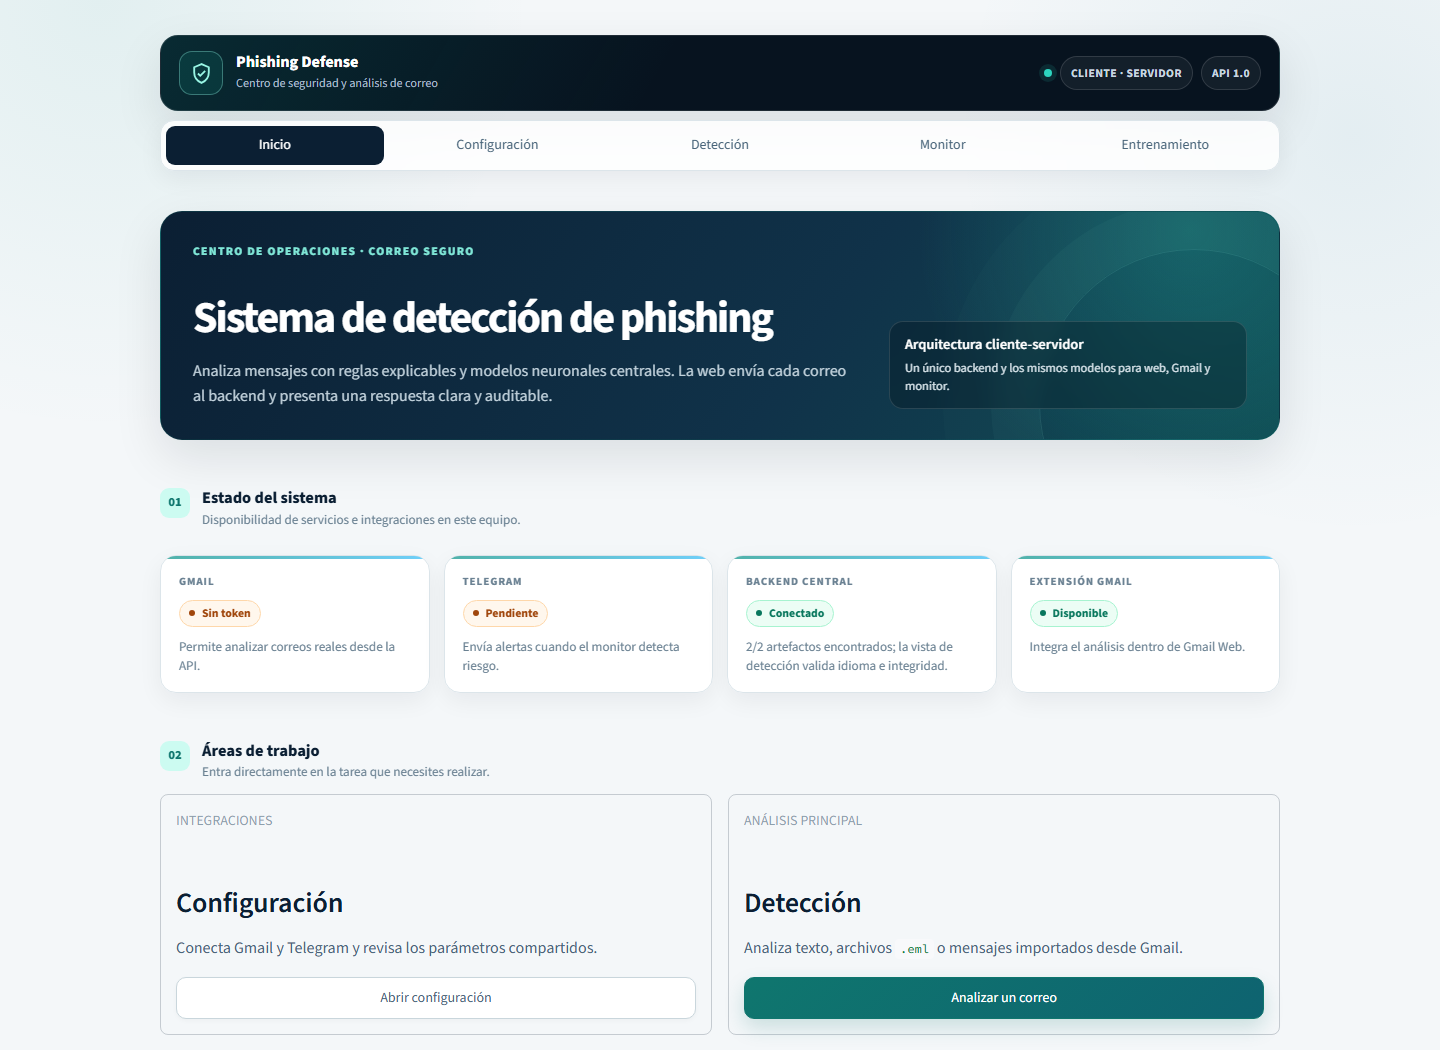
\includegraphics[width=0.92\textwidth]{latex_figures/figura_6_1.png}
  \caption[Pantalla inicial del cliente web con el backend central conectado.]{Pantalla inicial del cliente web con el backend central conectado. Fuente: elaboración propia.}
  \label{fig:6-1}
\end{figure}

\begin{figure}[H]
  \centering
  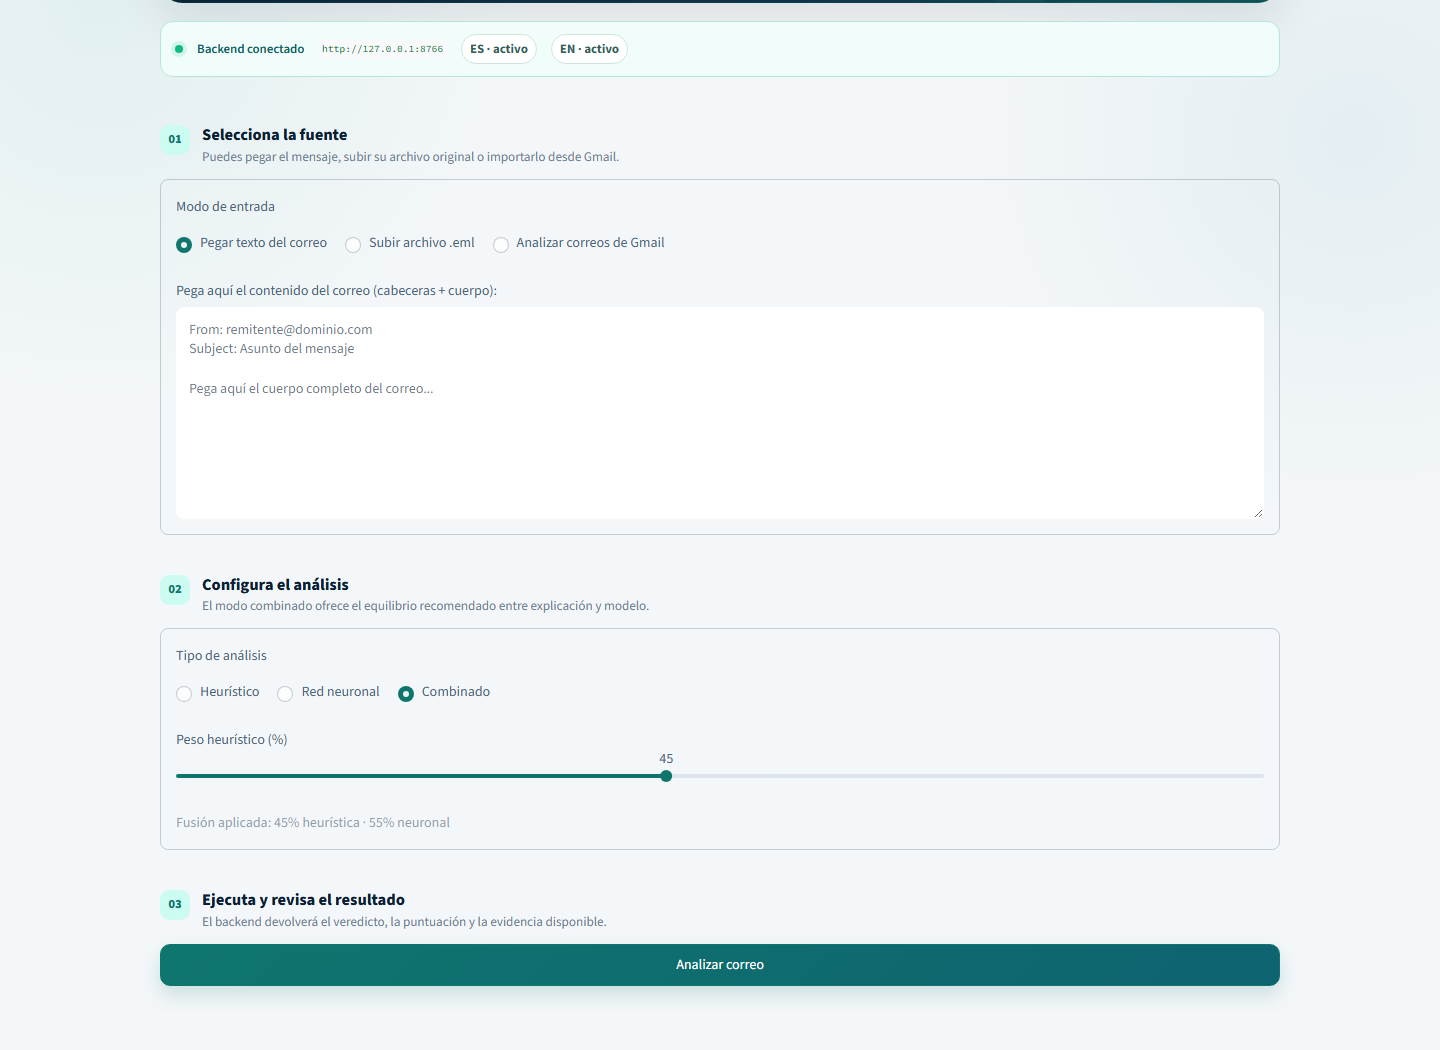
\includegraphics[width=0.92\textwidth]{latex_figures/figura_6_2.png}
  \caption[Fuentes de entrada y configuración del modo combinado en el cliente web.]{Fuentes de entrada y configuración del modo combinado en el cliente web. Fuente: elaboración propia.}
  \label{fig:6-2}
\end{figure}

\begin{figure}[H]
  \centering
  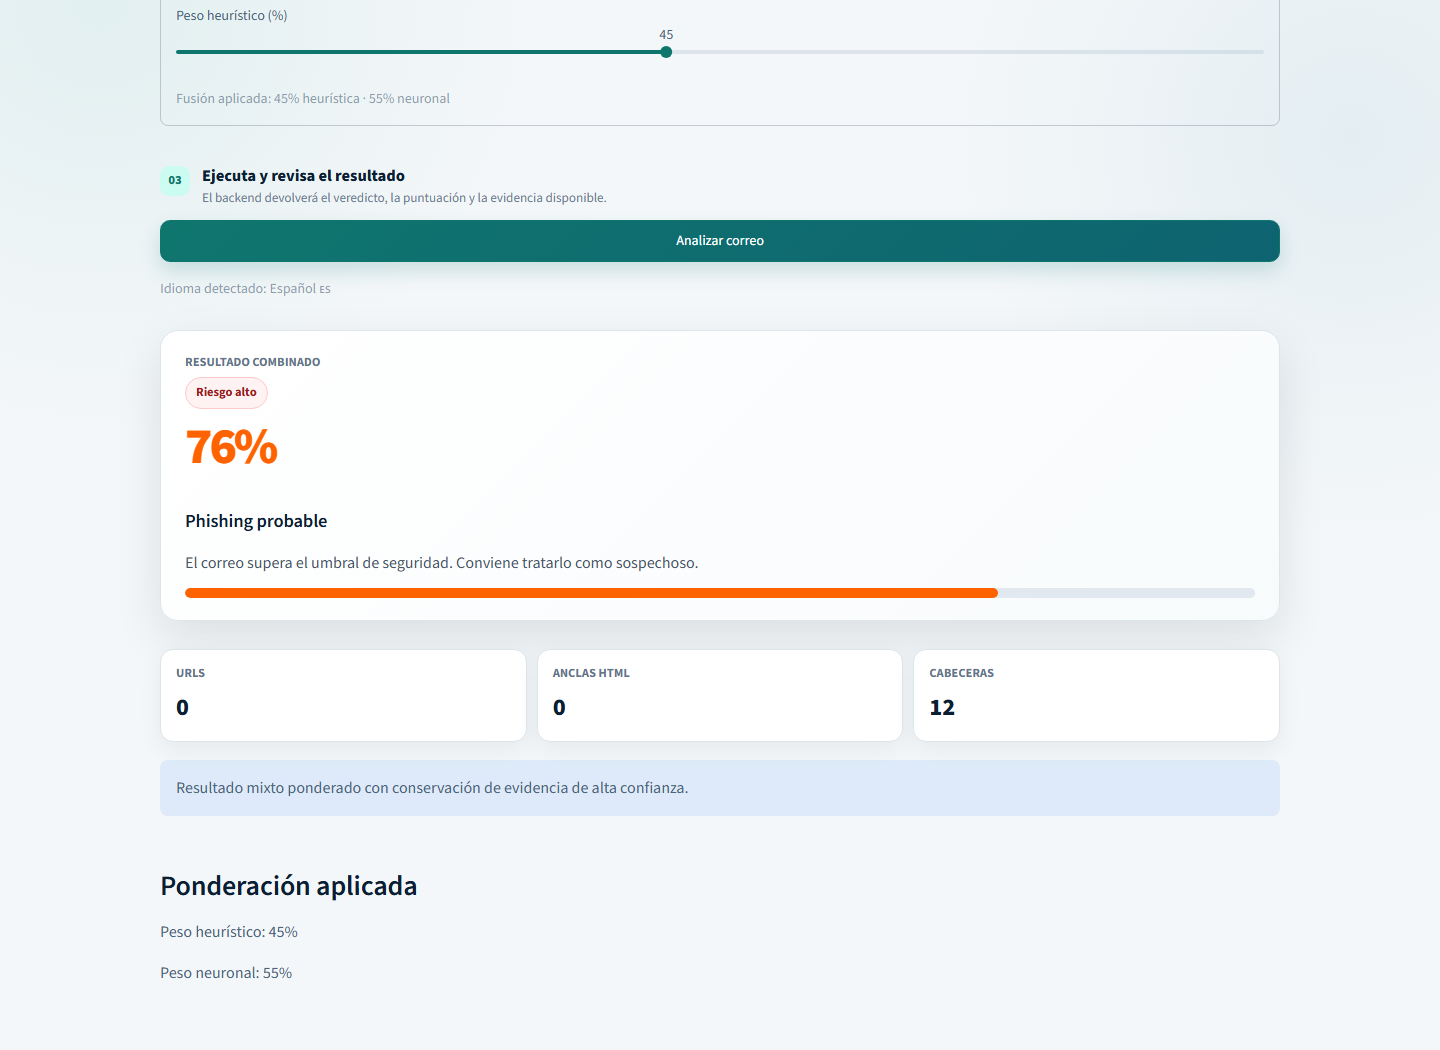
\includegraphics[width=0.92\textwidth]{latex_figures/figura_6_3.png}
  \caption[Resultado combinado del escenario BEC sintético reservado.]{Resultado combinado del escenario BEC sintético reservado. Fuente: elaboración propia.}
  \label{fig:6-3}
\end{figure}

\begin{figure}[H]
  \centering
  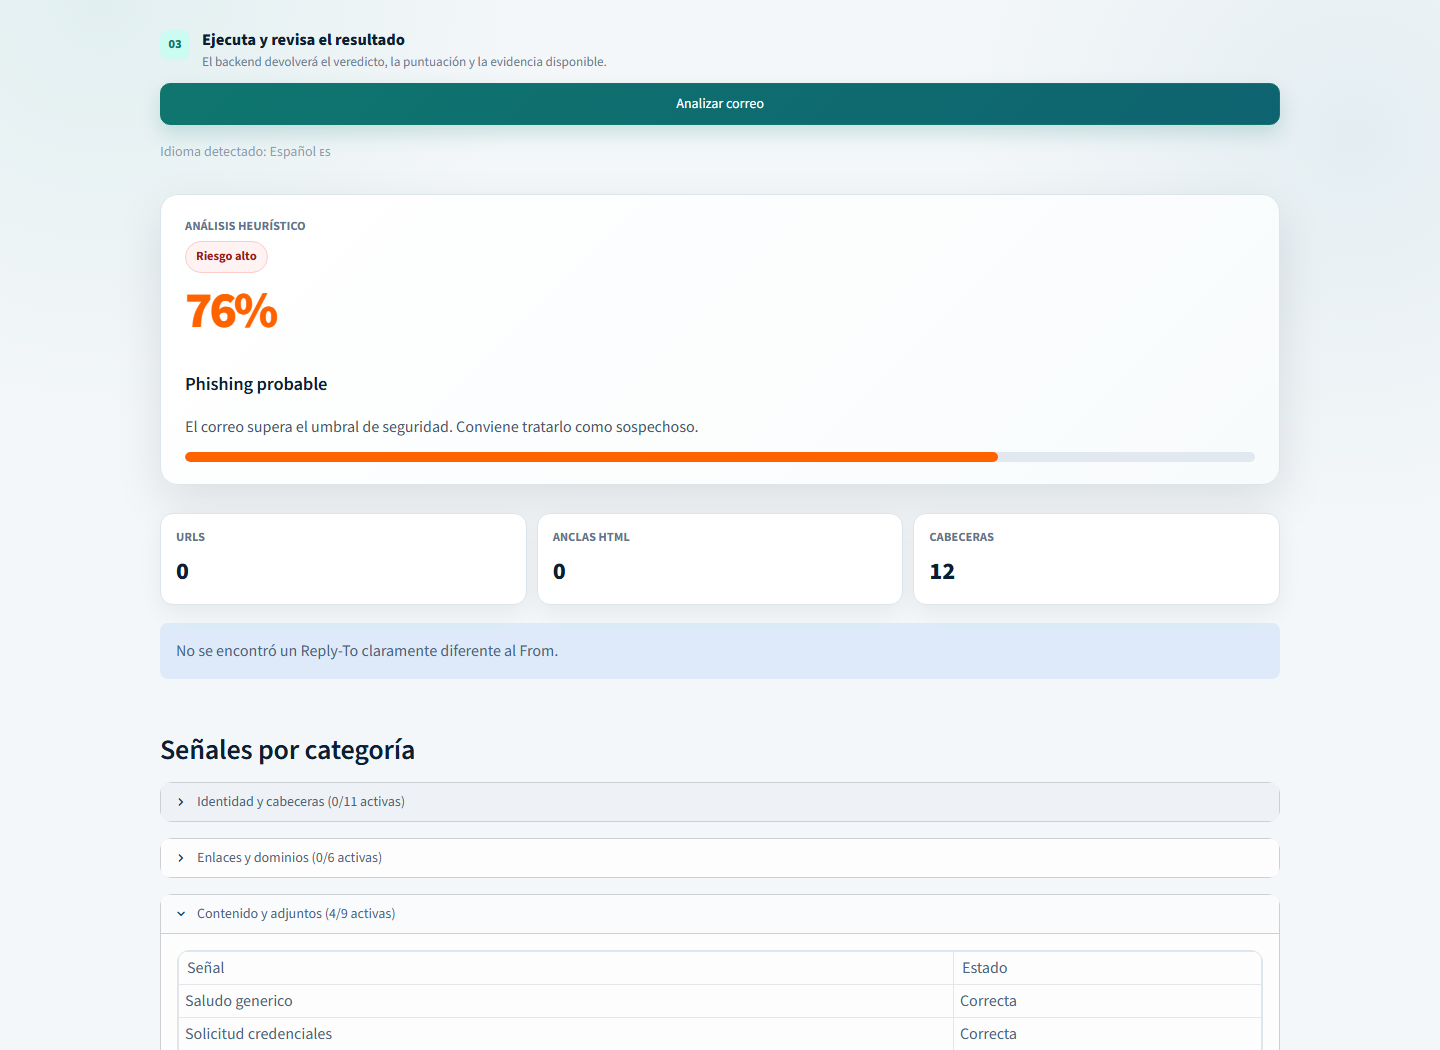
\includegraphics[width=0.92\textwidth]{latex_figures/figura_6_4.png}
  \caption[Resultado heurístico y desglose explicable de señales por categoría.]{Resultado heurístico y desglose explicable de señales por categoría. Fuente: elaboración propia.}
  \label{fig:6-4}
\end{figure}

\begin{figure}[H]
  \centering
  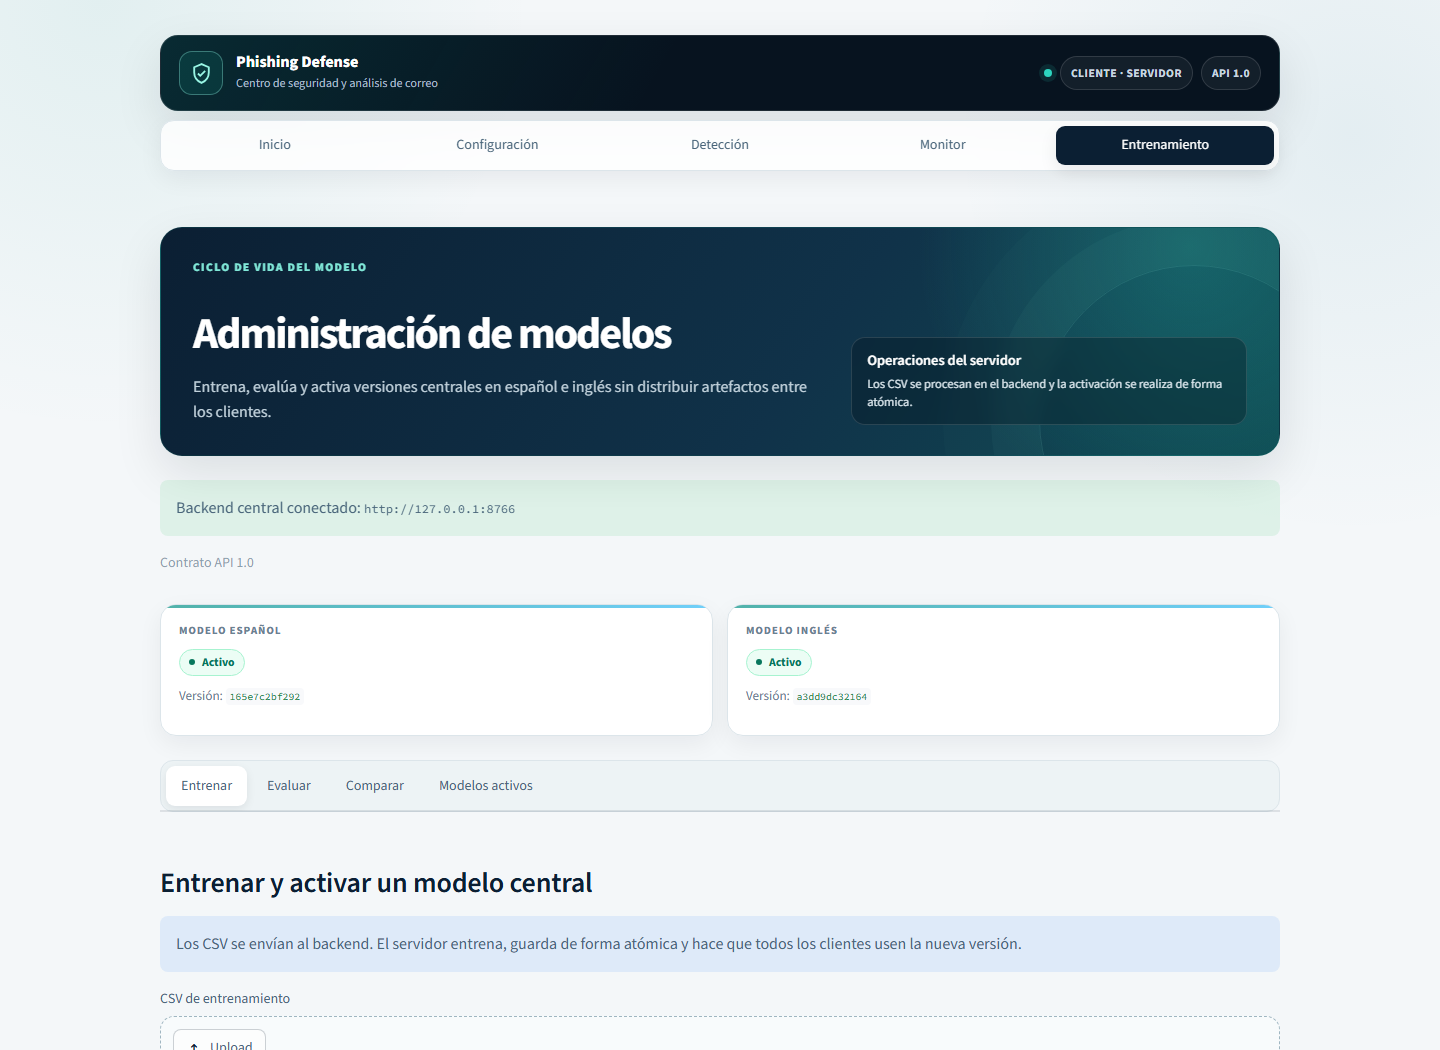
\includegraphics[width=0.92\textwidth]{latex_figures/figura_6_5.png}
  \caption[Administración y versiones activas de los modelos centrales ES y EN.]{Administración y versiones activas de los modelos centrales ES y EN. Fuente: elaboración propia.}
  \label{fig:6-5}
\end{figure}

\begin{figure}[H]
  \centering
  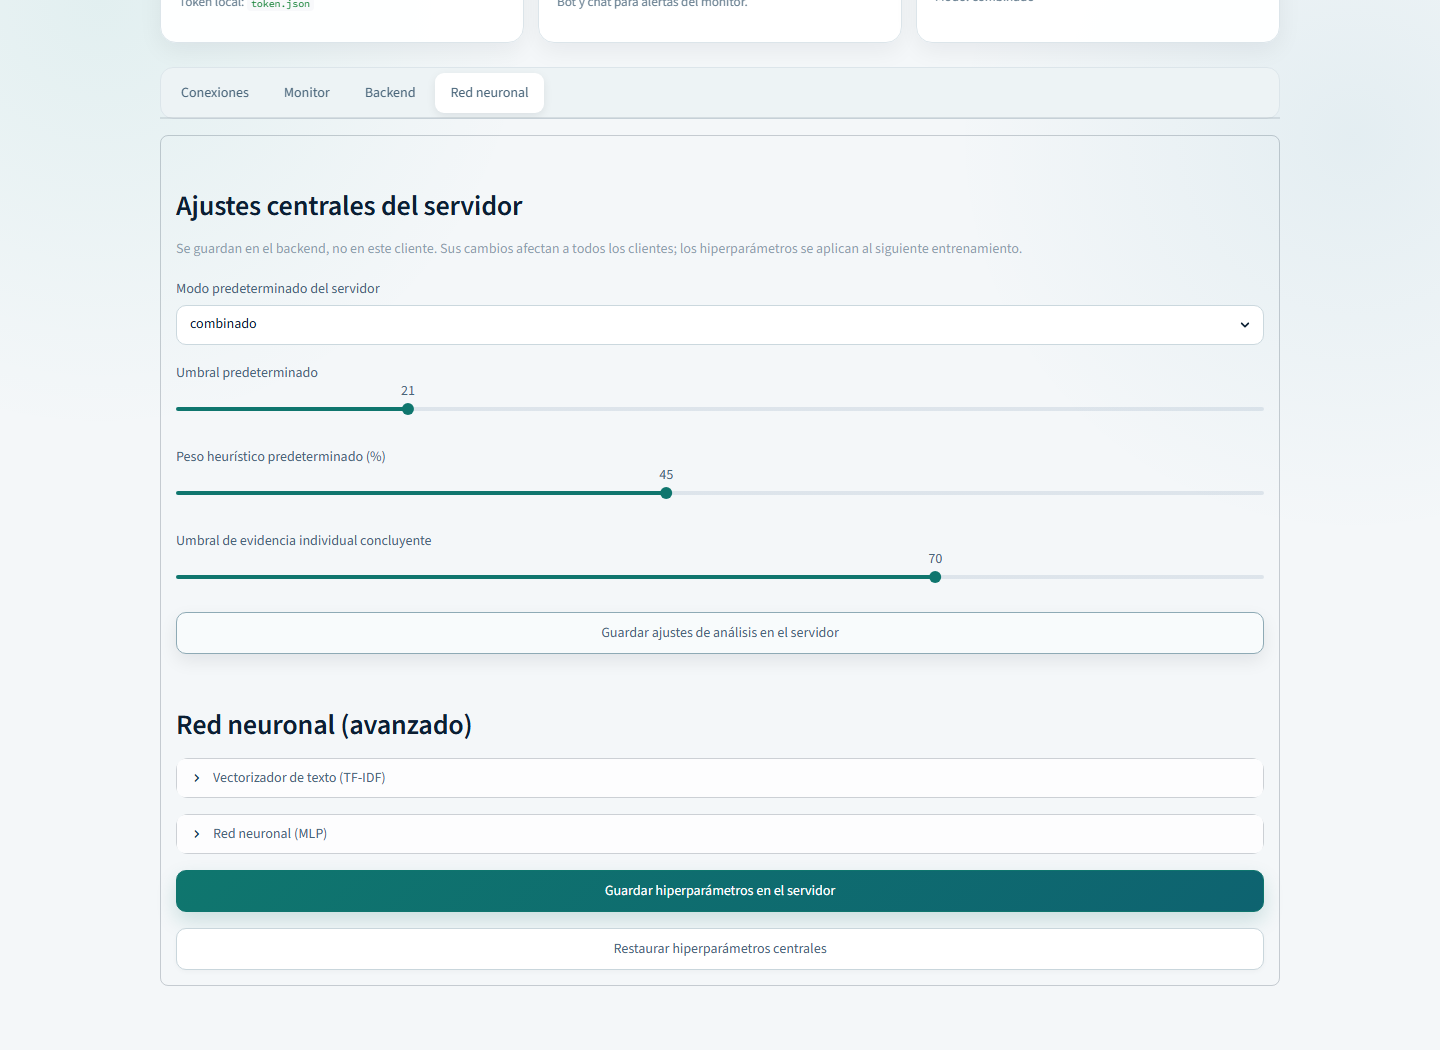
\includegraphics[width=0.92\textwidth]{latex_figures/figura_6_6.png}
  \caption[Ajustes de análisis e hiperparámetros almacenados en el servidor.]{Ajustes de análisis e hiperparámetros almacenados en el servidor. Fuente: elaboración propia.}
  \label{fig:6-6}
\end{figure}

\section{Discusión}

Los resultados confirman el diseño como base funcional: en los 16 EML reservados, el heurístico obtiene 100,0 \% de accuracy y recall; el combinado detecta los ocho phishing, incluido BEC sin enlace, con 87,5 \% de accuracy y dos falsos positivos; el neuronal conserva un falso negativo y dos falsos positivos. En DIFrauD el combinado logra 89,0 \% de accuracy y 93,4 \% de recall. La diferencia entre el holdout inglés interno (98,4 \%) y las validaciones externas muestra cambio de distribución. La limitación principal es la independencia, actualidad y validez de constructo de los datos, además de los controles de producción.

En el conjunto final de 16 EML, combinar detectores no mejora al heurístico: ambos detectan los ocho correos de phishing, pero la fusión añade dos falsas alarmas. Es una desventaja observada y debe reconocerse. El conjunto contiene escenarios locales reservados, con cabeceras, enlaces y patrones que las reglas inspeccionan; verifica funciones concretas y no representa la diversidad de una bandeja de entrada real. Con 16 mensajes, un solo error cambia la exactitud en 6,25 puntos porcentuales.

El interés del modo combinado es estudiar cómo integrar evidencia estructural explicable y patrones léxicos aprendidos, manteniendo disponibles los tres modos para compararlos. Esa complementariedad es una motivación de diseño, no una mejora universal demostrada. Para justificar su preferencia operativa haría falta evaluar los modos sobre el mismo corpus reciente e independiente y comparar tanto la detección como el coste de las falsas alarmas. El diagnóstico externo tampoco resuelve por sí solo esta cuestión, debido al posible solapamiento de fuentes y a la ausencia de cabeceras completas.

\chapter{Conclusiones generales}

El trabajo cumple los objetivos académicos y materializa un prototipo funcional dentro del alcance revisado. El cumplimiento de los compromisos originales es parcial: no se han integrado servicios externos de reputación, comprobación de certificados ni análisis activo de sitios web, como se detalla en el apartado~\ref{sec:objetivos-propuesta}. Dentro del alcance desarrollado, se ha estudiado el phishing desde su base psicológica y su evolución reciente, se ha revisado la investigación en machine learning y deep learning y se ha desarrollado un sistema cliente-servidor funcional que combina análisis heurístico explicable con un clasificador TF-IDF + MLP. Streamlit, la extensión de Gmail y el monitor envían las entradas al backend central, que procesa el correo y mantiene los modelos compartidos.

La valoración siguiente corresponde a los objetivos específicos de la introducción y debe leerse junto con la trazabilidad de la propuesta aprobada:

El primer objetivo, analizar el fenómeno del phishing, sus fases, tipologías y evolución histórica, se aborda en el marco teórico mediante modelos de fases, vectores de ataque, modalidades según personalización y técnicas emergentes contrastadas con fuentes académicas e informes de industria.

El segundo objetivo, estudiar los fundamentos psicológicos de la ingeniería social, se cubre mediante el análisis de los principios de Cialdini, los sesgos cognitivos de Kahneman y Tversky y el impacto de la inteligencia artificial generativa.

El tercer objetivo, revisar el estado del arte en técnicas de detección, se desarrolla en la sección dedicada a machine learning clásico, deep learning, transformers y enfoques híbridos, y concluye con el hueco de investigación que justifica el prototipo.

El cuarto objetivo, diseñar e implementar un sistema heurístico explicable y un clasificador TF-IDF + MLP, se materializa en el motor de señales sobre cabeceras, contenido, URLs y HTML y en el pipeline neuronal entrenable en español e inglés.

El quinto objetivo, integrar la aplicación con Gmail y proporcionar alertas mediante Telegram, se cumple mediante OAuth de solo lectura y el monitor opcional. Los mensajes autorizados se envían al backend central y Telegram recibe únicamente la alerta configurada; ni Streamlit ni el monitor duplican la lógica de análisis.

El sexto objetivo, evaluar el comportamiento del sistema, se aborda con 94 pruebas Python, 2 recorridos Chromium ---incluido web a backend---, benchmark reproducible, calibración separada de 40 casos, 16 EML reservados y 1.528 textos externos con hashes, matriz de confusión y errores por identificador. La estimación independiente sobre correo real reciente sigue delimitada como trabajo pendiente.

Entre los logros principales destacan la arquitectura cliente-servidor, una versión activa por idioma compartida por todos los clientes, activación atómica, Gmail/Telegram, pruebas Python y de navegador, CI, reentrenamiento reproducible, calibración separada, detección BEC y evaluación trazable local/externa. La carga diferida reduce históricamente el arranque de heurísticas un 96,6 \% y el de la aplicación un 76,2 \%. La fusión 45/55 conserva evidencia de alta confianza.

\section{Trabajo futuro}

Como trabajo futuro prioritario se plantea confirmar la calibración sobre datasets reales, recientes e independientes en español e inglés, con licencia, procedencia temporal y deduplicación frente al entrenamiento, y ampliar la detección BEC más allá de los patrones actuales. También se estudiarán ataques adversariales, transformers/LLM, reputación de dominios, análisis dinámico y etiquetado seguro. Un despliegue multiusuario requerirá autenticación, TLS, rate limiting, secretos e aislamiento de sesiones.

\chapter*{Glosario}
\addcontentsline{toc}{chapter}{Glosario}

\begin{description}[style=nextline,leftmargin=3.3cm]

  \item[API] Interfaz de operaciones que permite a un cliente enviar datos al backend mediante un contrato HTTP; Gmail y Telegram son integraciones externas distintas.
  \item[Aplicación web cliente-servidor] El navegador usa Streamlit como capa de presentación y Streamlit llama por HTTP al backend central obligatorio. En la configuración académica ambos procesos se ejecutan en el mismo equipo; la extensión y el monitor consumen el mismo contrato.
  \item[Blacklist (lista negra)] Lista local de dominios o URLs considerados no confiables que el sistema consulta durante el análisis.
  \item[Business Email Compromise (BEC)] Fraude que suplanta a directivos o proveedores para autorizar pagos o transferencias fraudulentas.
  \item[DKIM] Mecanismo de autenticación de correo basado en firmas criptográficas del dominio remitente.
  \item[SPF] Política DNS que permite comprobar si la IP emisora está autorizada para el dominio del sobre SMTP. No autentica por sí sola el From visible ni garantiza la integridad del contenido.
  \item[DMARC] Política e informes del dominio del From visible. Exige alineación con al menos un SPF o DKIM válido y puede solicitar none, quarantine o reject; no verifica por sí mismo el contenido del mensaje.
  \item[Análisis combinado] Modo que pondera ambas puntuaciones y conserva el máximo individual si alcanza el umbral de alta confianza. Produce un índice de riesgo, no una probabilidad calibrada.
  \item[Streamlit] Framework de Python utilizado para construir la interfaz web interactiva del prototipo.
  \item[Heurística] Conjunto de reglas basadas en conocimiento experto que evalúan indicios de phishing de forma explicable.
  \item[MLPClassifier] Perceptrón multicapa de scikit-learn: red neuronal de alimentación directa con una o más capas ocultas.
  \item[OAuth] Protocolo de autorización empleado para acceder a la API de Gmail sin compartir la contraseña.
  \item[Phishing] Técnica de ingeniería social que suplanta entidades legítimas para obtener información sensible.
  \item[Precisión] Proporción de casos clasificados como phishing que realmente lo son.
  \item[Quishing] Variante de phishing que utiliza códigos QR como vector de entrega.
  \item[Recall] Proporción de los casos de phishing reales que el modelo detecta correctamente.
  \item[Smishing] Variante de phishing mediante mensajes SMS.
  \item[TF-IDF] Técnica de vectorización de texto que pondera la frecuencia de cada término según su importancia.
  \item[Umbral (threshold)] Valor de puntuación a partir del cual un correo se considera phishing probable.
  \item[Vishing] Variante de phishing mediante llamadas telefónicas.
\end{description}

\clearpage
\addcontentsline{toc}{chapter}{Referencias}
\begin{thebibliography}{99}
\small
\setlength{\itemsep}{3pt}
\setlength{\parsep}{0pt}
\bibitem{ref1} AlEroud, A., \& Karabatis, G. (2020). Bypassing detection of URL-based phishing attacks using generative adversarial deep neural networks. In \emph{Proceedings of the Sixth International Workshop on Security and Privacy Analytics (IWSPA '20)} (pp. 53-60). ACM. \url{https://doi.org/10.1145/3375708.3380315}

\bibitem{ref2} Alghenaim, M., Alkawsi, G., \& Barnhart, C. R. (2025). The state of the art in AI-based phishing detection: A systematic literature review. In M. A. Al-Sharafi, M. Al-Emran, M. A. Mahmoud, \& I. Arpaci (Eds.), \emph{Current and Future Trends on AI Applications} (Studies in Computational Intelligence, Vol. 1178, pp. 431-458). Springer. \url{https://doi.org/10.1007/978-3-031-75091-5_23}

\bibitem{ref3} Al-Subaiey, A., Al-Thani, M., Alam, N. A., Antora, K. F., Khandakar, A., \& Zaman, S. A. U. (2024). Novel interpretable and robust web-based AI platform for phishing email detection. Computers and Electrical Engineering, 118, 109625. \url{https://doi.org/10.1016/j.compeleceng.2024.109625} Dataset: \url{https://www.kaggle.com/datasets/naserabdullahalam/phishing-email-dataset}

\bibitem{ref4} Alkhalil, Z., Hewage, C., Nawaf, L., \& Khan, I. (2021). Phishing attacks: A recent comprehensive study and a new anatomy. Frontiers in Computer Science, 3, Article 563060. \url{https://doi.org/10.3389/fcomp.2021.563060}

\bibitem{ref5} Altwaijry, N., Al-Turaiki, I., Alotaibi, R., \& Alakeel, F. (2024). Advancing phishing email detection: A comparative study of deep learning models. Sensors, 24(7), 2077. \url{https://doi.org/10.3390/s24072077}

\bibitem{ref6} Anti-Phishing Working Group. (2025). Phishing Activity Trends Report -- 2nd Quarter 2025. \url{https://docs.apwg.org/reports/apwg_trends_report_q2_2025.pdf}

\bibitem{ref7} Boumber, D. A., Qachfar, F. Z., \& Verma, R. (2024). Domain-agnostic adapter architecture for deception detection: Extensive evaluations with the DIFrauD benchmark. In Proceedings of the 2024 Joint International Conference on Computational Linguistics, Language Resources and Evaluation (LREC-COLING 2024) (pp. 5260-5274). ELRA and ICCL. \url{https://aclanthology.org/2024.lrec-main.468/}

\bibitem{ref8} Cialdini, R. B. (1984). Influence: The Psychology of Persuasion. William Morrow.

\bibitem{ref9} Federal Bureau of Investigation. (2024). 2023 Internet Crime Report. Internet Crime Complaint Center. \url{https://www.ic3.gov/Media/PDF/AnnualReport/2023_IC3Report.pdf}

\bibitem{ref10} Fortinet. (2025). 19 types of phishing attacks with examples. \url{https://www.fortinet.com/resources/cyberglossary/types-of-phishing-attacks}

\bibitem{ref12} Hadnagy, C. (2018). \emph{Social Engineering: The Science of Human Hacking} (2nd ed.). Wiley.

\bibitem{ref13} Heiding, F., Schneier, B., Vishwanath, A., Bernstein, J., \& Park, P. S. (2024). Devising and detecting phishing emails using large language models. IEEE Access, 12, 42131-42146. \url{https://doi.org/10.1109/ACCESS.2024.3375882}

\bibitem{ref15} Hutchinson, S., Zhang, Z., \& Liu, Q. (2018). Detecting phishing websites with random forest. In \emph{Machine Learning and Intelligent Communications} (pp. 470-479). Springer. \url{https://doi.org/10.1007/978-3-030-00557-3_46}

\bibitem{ref16} IBM. (2025). Cost of a Data Breach Report 2025. \url{https://www.ibm.com/think/x-force/2025-cost-of-a-data-breach-navigating-ai}

\bibitem{ref17} Imperva. (2023). What is phishing: Attack techniques \& scam examples. \url{https://www.imperva.com/learn/application-security/phishing-attack-scam/}

\bibitem{ref18} Instituto Nacional de Ciberseguridad. (2025). Balance de ciberseguridad 2024. \url{https://www.incibe.es/sites/default/files/Comunicación_2025/Infografía_BalanceCiberseguridad_INCIBE_2024_web.pdf}

\bibitem{ref19} Iván, A. (2026). SMS Spam Mexico - Dataset en Español Mexicano [Conjunto de datos]. Kaggle. \url{https://www.kaggle.com/datasets/aldoivan/sms-spam-mexico-dataset-en-espaol-mexicano}

\bibitem{ref20} Kahneman, D. (2011). Thinking, Fast and Slow. Farrar, Straus and Giroux.

\bibitem{ref21} Koide, T., Fukushi, N., Nakano, H., \& Chiba, D. (2024). ChatSpamDetector: Leveraging large language models for effective phishing email detection. arXiv preprint arXiv:2402.18093. \url{https://arxiv.org/abs/2402.18093}

\bibitem{ref22} Kroll. (2025). Q4 2024 Cyber Threat Landscape Report: CorruptQR Campaign. \url{https://www.kroll.com/en/reports/cyber/threat-intelligence-reports/q4-2024-threat-landscape-report-phishing}

\bibitem{ref23} Kuikel, S., Piplai, A., \& Aggarwal, P. (2025). Evaluating large language models for phishing detection, self-consistency, faithfulness, and explainability. arXiv preprint arXiv:2506.13746. \url{https://arxiv.org/abs/2506.13746}

\bibitem{ref24} Le, H., Pham, Q., Sahoo, D., \& Hoi, S. C. H. (2018). URLNet: Learning a URL representation with deep learning for malicious URL detection. arXiv preprint arXiv:1802.03162. \url{https://arxiv.org/abs/1802.03162}

\bibitem{ref25} Miltchev, R., Rangelov, D., \& Genchev, E. (2024). Phishing validation emails dataset [Conjunto de datos]. Zenodo. \url{https://doi.org/10.5281/zenodo.13474746}

\bibitem{ref26} Microsoft. (2025). Microsoft Digital Defense Report 2025. \url{https://www.microsoft.com/en-us/corporate-responsibility/cybersecurity/microsoft-digital-defense-report-2025/}

\bibitem{ref27} MITRE. (2025). ATT\&CK Framework: T1566 Phishing. \url{https://attack.mitre.org/techniques/T1566/}

\bibitem{ref28} Popescul, D., \& Radu, L. D. (2025). AI in phishing detection: A bibliometric review. Frontiers in Artificial Intelligence, 8, 1496580. \url{https://doi.org/10.3389/frai.2025.1496580}

\bibitem{ref29} Proofpoint. (2025). The Human Factor 2025: Vol. 1 Social Engineering. \url{https://www.proofpoint.com/us/resources/threat-reports/human-factor-social-engineering}

\bibitem{ref30} Rojas-Galeano, S. (2024). Zero-shot spam email classification using pre-trained large language models. arXiv preprint arXiv:2405.15936. \url{https://arxiv.org/abs/2405.15936}

\bibitem{ref31} Sánchez-Paniagua, M., Fidalgo, E., Alegre, E., \& Alaiz-Rodríguez, R. (2022). Phishing websites detection using a novel multipurpose dataset and web technologies features. Expert Systems with Applications, 207, 118010. \url{https://doi.org/10.1016/j.eswa.2022.118010}

\bibitem{ref32} Softecapps. (2024). Spam/ham Spanish [Conjunto de datos]. Hugging Face. \url{https://doi.org/10.57967/hf/2264}

\bibitem{ref14} Sulander, P. (2022). The three steps and five effects of the phishing attack kill chain. Hoxhunt. \url{https://hoxhunt.com/blog/three-steps-and-five-effects-of-the-phishing-attack-kill-chain}

\bibitem{ref33} Thakur, K., Ali, M. L., Obaidat, M. A., \& Kamruzzaman, A. (2023). A systematic review on deep-learning-based phishing email detection. Electronics, 12(21), 4545. \url{https://www.mdpi.com/2079-9292/12/21/4545}

\bibitem{ref34} Trad, F., \& Chehab, A. (2024). Prompt engineering or fine-tuning? A case study on phishing detection with large language models. Machine Learning and Knowledge Extraction, 6(1), 367-384. \url{https://doi.org/10.3390/make6010018}

\bibitem{ref35} Tversky, A., \& Kahneman, D. (1974). Judgment under uncertainty: Heuristics and biases. Science, 185(4157), 1124-1131. \url{https://doi.org/10.1126/science.185.4157.1124}

\bibitem{ref36} Uddin, M. A., Mahiuddin, M., \& Sarker, I. H. (2024). An explainable transformer-based model for phishing email detection: A large language model approach. arXiv preprint arXiv:2402.13871. \url{https://arxiv.org/abs/2402.13871}

\bibitem{ref37} Verizon. (2025). 2025 Data Breach Investigations Report. \url{https://www.verizon.com/business/resources/reports/2025-dbir-data-breach-investigations-report.pdf}

\bibitem{ref38} Wang, Y., Zhu, W., Xu, H., Qin, Z., Ren, K., \& Ma, W. (2023). A large-scale pretrained deep model for phishing URL detection. In \emph{ICASSP 2023 - 2023 IEEE International Conference on Acoustics, Speech and Signal Processing (ICASSP)} (pp. 1-5). IEEE. \url{https://doi.org/10.1109/ICASSP49357.2023.10095719}

\bibitem{ref39} Yerima, S. Y., \& Alzaylaee, M. K. (2020). High accuracy phishing detection based on convolutional neural networks. In \emph{Proceedings of the 3rd International Conference on Computer Applications \& Information Security} (pp. 1-6). IEEE. \url{https://doi.org/10.1109/ICCAIS48893.2020.9096869}

\end{thebibliography}

\appendix
\chapter*{Anexos}
\addcontentsline{toc}{chapter}{Anexos}

Este capítulo reúne el material complementario del Trabajo Fin de Grado: la estructura completa del repositorio, los fragmentos de código fuente más representativos del sistema y una guía resumida de instalación y uso. El código completo, las dependencias fijadas, los scripts de evaluación y las instrucciones se encuentran en el repositorio público \url{https://github.com/villarrubi/TFG}.

\chapter{Estructura del repositorio}

La siguiente estructura recoge los componentes principales de la aplicación cliente-servidor, sus clientes y el backend central de análisis:

\textbf{Estructura de directorios del repositorio}

\begin{lstlisting}
TFG/
|-- src/
|   |-- app.py                       # Entrada principal de Streamlit
|   |-- backend_server.py             # Servidor HTTP central
|   |-- config_app.py                 # Configuración de clientes y servidor
|   |-- detect_app.py                 # Cliente web de detección
|   |-- gmail_extension_server.py     # Proxy legado opcional (puerto 8767)
|   |-- monitor_app.py                # Vista de monitorización de Gmail
|   |-- monitor_gmail.py              # Monitorización periódica opcional
|   |-- train_app.py                  # Entrenamiento y evaluación
|   |-- ui_components.py              # Componentes visuales compartidos
|   `-- sistema_phishing/
|       |-- analizador_email.py       # Parseo y normalización de correos
|       |-- analysis_service.py       # Coordinación del análisis en servidor
|       |-- analyzer.py               # Orquestador heurístico
|       |-- backend_service.py        # Casos de uso del servidor central
|       |-- backend_client.py         # Cliente HTTP compartido
|       |-- model_config.py           # Configuración ML ligera para clientes
|       |-- file_utils.py             # Escrituras atómicas de secretos y estado
|       |-- network.py                # Política de loopback y bind
|       |-- configuracion.py           # Configuración del dominio
|       |-- content_signals.py        # Señales de texto y adjuntos
|       |-- correo.py                 # Representación interna común
|       |-- dataset.py                # Normalización de CSV
|       |-- env_loader.py             # Variables locales de entorno
|       |-- explanations.py           # Explicaciones del riesgo
|       |-- gmail_client.py            # Integración OAuth con Gmail
|       |-- gmail_monitor.py           # Lógica de monitorización
|       |-- header_signals.py          # Cabeceras y autenticación
|       |-- heuristicas.py             # Fachada heurística
|       |-- html_signals.py            # Señales HTML
|       |-- http_api.py                # Transporte HTTP y validación
|       |-- idioma.py                  # Detección de idioma
|       |-- metrics.py                 # Métricas y matriz de confusión
|       |-- modelo_neural.py           # Pipeline TF-IDF + MLP
|       |-- neural.py                  # Fachada neuronal
|       |-- scorer.py                  # Cálculo de puntuación
|       |-- signal_builder.py          # Construcción de señales
|       |-- signals.py                 # Utilidades de señales
|       |-- telegram_notifier.py       # Alertas por Telegram
|       `-- url_utils.py               # Análisis de URLs
|-- tests/                            # Suite unittest
|-- scripts/                          # Automatización y experimentos
|-- requirements.txt
|-- credentials.example.json
|-- config/                            # Plantillas cliente/servidor
`-- runtime/                           # Datos persistentes separados
    |-- client/                       # Secretos y preferencias (Git ignora)
    `-- server/                       # Ajustes y modelos centrales
        `-- models/                   # Artefactos ES/EN
\end{lstlisting}

\chapter{Fragmentos de código fuente}

A continuación se presentan extractos simplificados para explicar las responsabilidades; se omiten validaciones, metadatos y métodos auxiliares. No son archivos ejecutables completos. El código íntegro y vigente se encuentra en el repositorio. Se muestran la fachada del análisis heurístico, el servicio común que combina heurística y red neuronal, y el núcleo del pipeline neuronal TF-IDF + MLP.

\section{Fachada del análisis heurístico (heuristicas.py)}

\begin{lstlisting}
heuristicas.py
"""Fachada de heurísticas para el sistema de detección de phishing."""
from .analyzer import PhishingAnalyzer
from .correo import CorreoAnalizado
from .url_utils import extraer_urls
__all__ = ["analizar_correo", "extraer_urls"]
def analizar_correo(correo):
    """Normaliza la entrada y delega el análisis en PhishingAnalyzer."""
    correo_analizado = CorreoAnalizado.from_input(correo)
    return PhishingAnalyzer(correo_analizado).analyze()
\end{lstlisting}

\section{Servicio común de análisis (analysis\_service.py)}

\begin{lstlisting}
analysis_service.py (extracto simplificado)
from collections.abc import Callable
from threading import Lock
from typing import Protocol
from .analizador_email import construir_texto_para_analisis
from .heuristicas import analizar_correo
from .idioma import detectar_idioma_correo
MODO_HEURISTICO = "heuristico"
MODO_NEURAL = "neural"
MODO_COMBINADO = "combinado"
def cargar_detector_neural(config, idioma="es"):
    # Importación diferida: el modo heurístico no carga scikit-learn.
    from .modelo_neural import ModelStorage, NeuralPhishingClassifier, NeuralPhishingDetector
    ruta_principal = config.model_path_en if idioma == "en" else config.model_path_es
    classifier = ModelStorage(ruta_principal).load()
    idioma_esperado = "english" if idioma == "en" else "spanish"
    if classifier is not None and getattr(classifier, "language", None) != idioma_esperado:
        classifier = None  # No reutilizar silenciosamente otro idioma.
    if classifier is None:
        classifier = NeuralPhishingClassifier(language=idioma_esperado)
        classifier.fit_default()
    return NeuralPhishingDetector(classifier)
class EmailAnalysisService:
    def __init__(self, config, heuristic_analyzer=None, detector_loader=None, language_detector=None):
        validar_configuracion(config)
        self.config = config
        self._heuristic_analyzer = heuristic_analyzer or analizar_correo
        self._detector_loader = detector_loader or cargar_detector_neural
        self._language_detector = language_detector or detectar_idioma_correo
        self._detectores = {}
        self._detector_lock = Lock()
    # _aplicar_umbral y construir_resultado_combinado validan el contrato y los pesos.
    def analyze(self, datos_email):
        if self.config.mode == MODO_HEURISTICO:
            return _aplicar_umbral(self._heuristic_analyzer(datos_email), self.config.threshold)
        resultado_neural = self._analyze_neural(datos_email)
        if self.config.mode == MODO_NEURAL:
            return _aplicar_umbral(resultado_neural, self.config.threshold)
        resultado_heur = self._heuristic_analyzer(datos_email)
        return construir_resultado_combinado(resultado_heur, resultado_neural, self.config)
    def analyze_all(self, datos_email):
        resultado_heur = _aplicar_umbral(self._heuristic_analyzer(datos_email), self.config.threshold)
        resultado_neural = _aplicar_umbral(self._analyze_neural(datos_email), self.config.threshold)
        resultado_combinado = construir_resultado_combinado(resultado_heur, resultado_neural, self.config)
        return {"heuristico": resultado_heur, "neural": resultado_neural, "combinado": resultado_combinado}
    def _analyze_neural(self, datos_email):
        texto = construir_texto_para_analisis(datos_email)
        idioma = self._language_detector(texto)
        detector = self._detectores.get(idioma)
        if detector is None:
            with self._detector_lock:
                detector = self._detectores.get(idioma)
                if detector is None:
                    detector = self._detector_loader(self.config, idioma)
                    self._detectores[idioma] = detector
        return detector.analyze(texto, datos_email.get("from", ""), datos_email.get("subject", ""))
\end{lstlisting}

\section{Núcleo del clasificador neuronal (modelo\_neural.py)}

\begin{lstlisting}
modelo_neural.py (extracto simplificado)
class NeuralPhishingClassifier:
    def __init__(self, language="spanish", hiperparametros=None):
        self.language = language
        hp = hiperparametros or cargar_hiperparametros_desde_env()
        self.pipeline = Pipeline([
            ("vectorizer", TfidfVectorizer(ngram_range=hp.tfidf_ngram_range, ...)),
            ("classifier", MLPClassifier(hidden_layer_sizes=hp.mlp_hidden_layer_sizes, ...)),
        ])
    def fit(self, textos, etiquetas):
        # Valida las etiquetas y entrena una ejecución nueva.
        self.pipeline.fit(textos, etiquetas)
    def predict_proba(self, texts):
        proba = self.pipeline.predict_proba(texts)
        clases = self.pipeline.named_steps["classifier"].classes_.tolist()
        indice_phishing = clases.index(1)
        return [float(fila[indice_phishing]) for fila in proba]
    def __getstate__(self):
        state = self.__dict__.copy()
        state["training_texts"] = []
        state["training_labels"] = []
        return state
class NeuralPhishingDetector:
    def __init__(self, classifier):
        self.classifier = classifier
    def analyze(self, texto, remitente="", subject=""):
        probability = self.classifier.predict_proba([texto])[0]
        return {
            "is_phishing": probability >= 0.5,
            "risk_score": round(probability * 100, 1),
            "description": "Clasificación basada en una red neuronal entrenada.",
            "from": remitente,
            "subject": subject,
        }
\end{lstlisting}

\chapter{Guía resumida de instalación y uso}

Este anexo resume la ejecución cliente-servidor local. Primero se inicia el backend obligatorio en 127.0.0.1:8766 y después Streamlit en 127.0.0.1:8501. Para una demostración desde un móvil de la misma red privada se mantiene la API en loopback y se inicia solo la web con streamlit run src/app.py --server.address 0.0.0.0 --server.port 8501; se accede mediante \url{http://IP_DEL_EQUIPO:8501} y puede ser necesario permitir el puerto 8501 en el perfil privado del firewall. No requiere --allow-remote ni abrir 8766. Como Streamlit no incorpora autenticación multiusuario, este acceso LAN debe ser temporal, en una red de confianza y sin redirección de puertos. La extensión apunta directamente al backend desde Opciones y el monitor usa PHISHING\_BACKEND\_URL. El puerto 8767 queda como proxy antiguo opcional. Un despliegue remoto real exige HTTPS y controles operativos adicionales.

\textbf{Comandos de instalación y uso}

\begin{lstlisting}
# 1. Crear y activar un entorno virtual
python -m venv .venv
.\.venv\Scripts\Activate.ps1
# 2. Instalar dependencias
python -m pip install -r requirements-dev.txt -c constraints.txt
# 3. Ejecutar primero el backend central
$env:PYTHONPATH="src"; python src/backend_server.py
# 3b. Ejecutar el cliente web en otra terminal
$env:PYTHONPATH="src"; streamlit run src/app.py
# 3c. El proxy 8767 solo se usa por compatibilidad antigua
$env:PYTHONPATH="src"; python src/gmail_extension_server.py
# 4. Ejecutar la suite de pruebas
$env:PYTHONPATH="src"; python -m unittest discover -s tests -p "test_*.py"
\end{lstlisting}

\section{Uso del prototipo}

La aplicación ofrece texto, EML y Gmail desde Streamlit, además del correo visible en la extensión. Todos esos clientes envían la entrada al backend central. /analyze acepta campos JSON o EML Base64 y devuelve riesgo, señales, explicación, idioma y versión para que cada cliente se limite a presentarlos.

Para cada correo, el sistema devuelve una puntuación global de riesgo, una clasificación y un desglose de señales. Interpreta los resultados SPF/DKIM/DMARC ya presentes en las cabeceras, sin consultas DNS ni validación criptográfica, y revisa coherencia del remitente, urgencia, URLs, IPs, punycode, acortadores, redirecciones, adjuntos e ingeniería social. Las señales activadas se acompañan de explicaciones para interpretar por qué se ha clasificado el mensaje.

El clasificador neuronal del backend asigna la probabilidad y selecciona el modelo por idioma. Streamlit recibe conjuntamente la puntuación neuronal y las señales heurísticas; no carga el pipeline ni recalcula la decisión.

Desde la vista Monitor se consultan correos de Gmail y se envían al backend. Si Telegram está configurado, el cliente puede alertar con el remitente, asunto y puntuación devueltos por el servidor.

Un caso habitual consiste en levantar backend y web, cargar un EML o pegar texto. El cliente envía la entrada, el servidor la procesa con la versión central y devuelve señales y riesgo. Para separar físicamente ambos lados se publica el backend detrás de HTTPS y se cambia PHISHING\_BACKEND\_URL; la latencia dependerá entonces también de la red.

\chapter{Lista de verificación de la validación}

La siguiente lista resume las comprobaciones realizadas sobre el prototipo durante la fase de validación, tal y como se detalla en el capítulo de pruebas y resultados.

\begin{itemize}
  \item Verificado: 94 pruebas Python y 2 recorridos reales con Chromium, incluido cliente web a backend.
\end{itemize}

Verificado: Benchmark reproducible de arranque e inferencia con comparación antes/después.

\begin{itemize}
  \item Verificado: Normalización correcta de etiquetas phishing y correo legítimo.
  \item Verificado: Entrenamiento del modelo TF-IDF + MLP en español e inglés.
  \item Verificado: calibración controlada de 40 casos y evaluación final de 16 EML locales reservados, con hashes, métricas y errores por caso; pendiente corpus real representativo.
  \item Verificado: Cálculo de exactitud, precisión, recall y F1.
  \item Verificado: arranque separado de backend y Streamlit, navegación y análisis HTTP completo.
  \item Verificado: Análisis desde texto pegado y archivo .eml.
  \item Verificado con dobles de prueba: importación de correos por el cliente de Gmail. La conexión OAuth real requiere credenciales de laboratorio y una comprobación separada.
  \item Verificado: Selección del modelo neuronal según el idioma del mensaje.
  \item Verificado con dobles de prueba: monitorización y notificación Telegram. Las pruebas locales no acreditan disponibilidad actual de los servicios externos.
\end{itemize}

\chapter{Resumen de arquitectura y evidencia}

El sistema es cliente-servidor. Streamlit, la extensión y el monitor son clientes HTTP; backend\_server.py centraliza parser, análisis, entrenamiento y una versión activa por idioma. En la configuración de defensa todos los procesos están en el mismo equipo y loopback, pero el servidor es obligatorio y puede separarse cambiando PHISHING\_BACKEND\_URL.

La evidencia reproducible comprende 94 pruebas Python, 2 recorridos con Chromium, integración continua, benchmark, calibración separada de 40 casos, evaluación de 16 EML reservados y diagnóstico de 1.528 textos DIFrauD. Los EML son sintéticos y DIFrauD conserva riesgo de solapamiento; ninguna cifra estima producción.

La persistencia se separa por propietario: runtime/client guarda las credenciales OAuth, el token, el estado del monitor y las preferencias de cada instalación; runtime/server guarda los ajustes centrales y los modelos ES/EN. GET/POST /settings permite administrarlos sin compartir el sistema de archivos del servidor.

\end{document}
